\documentclass[]{book}
\usepackage{lmodern}
\usepackage{amssymb,amsmath}
\usepackage{ifxetex,ifluatex}
\usepackage{fixltx2e} % provides \textsubscript
\ifnum 0\ifxetex 1\fi\ifluatex 1\fi=0 % if pdftex
  \usepackage[T1]{fontenc}
  \usepackage[utf8]{inputenc}
\else % if luatex or xelatex
  \ifxetex
    \usepackage{mathspec}
  \else
    \usepackage{fontspec}
  \fi
  \defaultfontfeatures{Ligatures=TeX,Scale=MatchLowercase}
\fi
% use upquote if available, for straight quotes in verbatim environments
\IfFileExists{upquote.sty}{\usepackage{upquote}}{}
% use microtype if available
\IfFileExists{microtype.sty}{%
\usepackage{microtype}
\UseMicrotypeSet[protrusion]{basicmath} % disable protrusion for tt fonts
}{}
\usepackage[margin=1in]{geometry}
\usepackage{hyperref}
\hypersetup{unicode=true,
            pdftitle={Bayesian Statistics},
            pdfauthor={Christine Chai},
            pdfborder={0 0 0},
            breaklinks=true}
\urlstyle{same}  % don't use monospace font for urls
\usepackage{natbib}
\bibliographystyle{apalike}
\usepackage{color}
\usepackage{fancyvrb}
\newcommand{\VerbBar}{|}
\newcommand{\VERB}{\Verb[commandchars=\\\{\}]}
\DefineVerbatimEnvironment{Highlighting}{Verbatim}{commandchars=\\\{\}}
% Add ',fontsize=\small' for more characters per line
\usepackage{framed}
\definecolor{shadecolor}{RGB}{248,248,248}
\newenvironment{Shaded}{\begin{snugshade}}{\end{snugshade}}
\newcommand{\KeywordTok}[1]{\textcolor[rgb]{0.13,0.29,0.53}{\textbf{#1}}}
\newcommand{\DataTypeTok}[1]{\textcolor[rgb]{0.13,0.29,0.53}{#1}}
\newcommand{\DecValTok}[1]{\textcolor[rgb]{0.00,0.00,0.81}{#1}}
\newcommand{\BaseNTok}[1]{\textcolor[rgb]{0.00,0.00,0.81}{#1}}
\newcommand{\FloatTok}[1]{\textcolor[rgb]{0.00,0.00,0.81}{#1}}
\newcommand{\ConstantTok}[1]{\textcolor[rgb]{0.00,0.00,0.00}{#1}}
\newcommand{\CharTok}[1]{\textcolor[rgb]{0.31,0.60,0.02}{#1}}
\newcommand{\SpecialCharTok}[1]{\textcolor[rgb]{0.00,0.00,0.00}{#1}}
\newcommand{\StringTok}[1]{\textcolor[rgb]{0.31,0.60,0.02}{#1}}
\newcommand{\VerbatimStringTok}[1]{\textcolor[rgb]{0.31,0.60,0.02}{#1}}
\newcommand{\SpecialStringTok}[1]{\textcolor[rgb]{0.31,0.60,0.02}{#1}}
\newcommand{\ImportTok}[1]{#1}
\newcommand{\CommentTok}[1]{\textcolor[rgb]{0.56,0.35,0.01}{\textit{#1}}}
\newcommand{\DocumentationTok}[1]{\textcolor[rgb]{0.56,0.35,0.01}{\textbf{\textit{#1}}}}
\newcommand{\AnnotationTok}[1]{\textcolor[rgb]{0.56,0.35,0.01}{\textbf{\textit{#1}}}}
\newcommand{\CommentVarTok}[1]{\textcolor[rgb]{0.56,0.35,0.01}{\textbf{\textit{#1}}}}
\newcommand{\OtherTok}[1]{\textcolor[rgb]{0.56,0.35,0.01}{#1}}
\newcommand{\FunctionTok}[1]{\textcolor[rgb]{0.00,0.00,0.00}{#1}}
\newcommand{\VariableTok}[1]{\textcolor[rgb]{0.00,0.00,0.00}{#1}}
\newcommand{\ControlFlowTok}[1]{\textcolor[rgb]{0.13,0.29,0.53}{\textbf{#1}}}
\newcommand{\OperatorTok}[1]{\textcolor[rgb]{0.81,0.36,0.00}{\textbf{#1}}}
\newcommand{\BuiltInTok}[1]{#1}
\newcommand{\ExtensionTok}[1]{#1}
\newcommand{\PreprocessorTok}[1]{\textcolor[rgb]{0.56,0.35,0.01}{\textit{#1}}}
\newcommand{\AttributeTok}[1]{\textcolor[rgb]{0.77,0.63,0.00}{#1}}
\newcommand{\RegionMarkerTok}[1]{#1}
\newcommand{\InformationTok}[1]{\textcolor[rgb]{0.56,0.35,0.01}{\textbf{\textit{#1}}}}
\newcommand{\WarningTok}[1]{\textcolor[rgb]{0.56,0.35,0.01}{\textbf{\textit{#1}}}}
\newcommand{\AlertTok}[1]{\textcolor[rgb]{0.94,0.16,0.16}{#1}}
\newcommand{\ErrorTok}[1]{\textcolor[rgb]{0.64,0.00,0.00}{\textbf{#1}}}
\newcommand{\NormalTok}[1]{#1}
\usepackage{longtable,booktabs}
\usepackage{graphicx,grffile}
\makeatletter
\def\maxwidth{\ifdim\Gin@nat@width>\linewidth\linewidth\else\Gin@nat@width\fi}
\def\maxheight{\ifdim\Gin@nat@height>\textheight\textheight\else\Gin@nat@height\fi}
\makeatother
% Scale images if necessary, so that they will not overflow the page
% margins by default, and it is still possible to overwrite the defaults
% using explicit options in \includegraphics[width, height, ...]{}
\setkeys{Gin}{width=\maxwidth,height=\maxheight,keepaspectratio}
\IfFileExists{parskip.sty}{%
\usepackage{parskip}
}{% else
\setlength{\parindent}{0pt}
\setlength{\parskip}{6pt plus 2pt minus 1pt}
}
\setlength{\emergencystretch}{3em}  % prevent overfull lines
\providecommand{\tightlist}{%
  \setlength{\itemsep}{0pt}\setlength{\parskip}{0pt}}
\setcounter{secnumdepth}{5}
% Redefines (sub)paragraphs to behave more like sections
\ifx\paragraph\undefined\else
\let\oldparagraph\paragraph
\renewcommand{\paragraph}[1]{\oldparagraph{#1}\mbox{}}
\fi
\ifx\subparagraph\undefined\else
\let\oldsubparagraph\subparagraph
\renewcommand{\subparagraph}[1]{\oldsubparagraph{#1}\mbox{}}
\fi

%%% Use protect on footnotes to avoid problems with footnotes in titles
\let\rmarkdownfootnote\footnote%
\def\footnote{\protect\rmarkdownfootnote}

%%% Change title format to be more compact
\usepackage{titling}

% Create subtitle command for use in maketitle
\newcommand{\subtitle}[1]{
  \posttitle{
    \begin{center}\large#1\end{center}
    }
}

\setlength{\droptitle}{-2em}
  \title{Bayesian Statistics}
  \pretitle{\vspace{\droptitle}\centering\huge}
  \posttitle{\par}
\subtitle{A Companion to the Statistics with R Coursera Course}
  \author{Christine Chai}
  \preauthor{\centering\large\emph}
  \postauthor{\par}
  \predate{\centering\large\emph}
  \postdate{\par}
  \date{Last built on 2017-11-23}

\usepackage{amsthm}
\usepackage{booktabs}


\makeatletter
\def\thm@space@setup{%
  \thm@preskip=8pt plus 2pt minus 4pt
  \thm@postskip=\thm@preskip
}
\makeatother

\usepackage{amsthm}
\newtheorem{theorem}{Theorem}[chapter]
\newtheorem{lemma}{Lemma}[chapter]
\theoremstyle{definition}
\newtheorem{definition}{Definition}[chapter]
\newtheorem{corollary}{Corollary}[chapter]
\newtheorem{proposition}{Proposition}[chapter]
\theoremstyle{definition}
\newtheorem{example}{Example}[chapter]
\theoremstyle{definition}
\newtheorem{exercise}{Exercise}[chapter]
\theoremstyle{remark}
\newtheorem*{remark}{Remark}
\newtheorem*{solution}{Solution}
\let\BeginKnitrBlock\begin \let\EndKnitrBlock\end
\begin{document}
\maketitle

{
\setcounter{tocdepth}{1}
\tableofcontents
}
\chapter*{Welcome}\label{welcome}
\addcontentsline{toc}{chapter}{Welcome}

\newcommand{\No}{\textsf{N}}
\newcommand{\Ga}{\textsf{Gamma}}
\newcommand{\St}{\textsf{t}}
\newcommand{\NoGa}{\textsf{NormalGamma}}
\newcommand{\BF}{\textsf{BF}}
\newcommand{\data}{\text{data}}
\newcommand{\iid}{\mathrel{\mathop{\sim}\limits^{\rm iid}}}
\newcommand{\Ca}{\textsf{C}}



This book is a written companion for the Coursera Course `Bayesian
Statistics' from the Statistics with R specialization. Materials and
examples from the course are discussed more extensively and extra
examples and exercises are provided.

\chapter{The Basics of Bayesian
Statistics}\label{the-basics-of-bayesian-statistics}

Bayesian statistics mostly involves \textbf{conditional probability},
which is the the probability of an event A \textbf{given} event B, and
it can be calculated using the Bayes' rule. The concept of conditional
probability is widely used in medical testing, in which false positives
and false negatives may occur. A false positive can be defined as a
positive outcome on a medical test when the patient does not actually
have the disease they are being tested for. In other words, it's the
probability of testing positive given no disease. Similarly, a false
negative can be defined as a negative outcome on a medical test when the
patient does have the disease. In other words, testing negative given
disease. Both indicators are critical for any medical decisions.

For how the Bayes' rule is applied, we can set up a prior, then
calculate posterior probabilities based on a prior and likelihood. That
is to say, the prior probabilities are updated through an iterative
process of data collection.

\section{Bayes' Rule}\label{bayes-rule}

This section introduces how the Bayes' rule is applied to calculating
conditional probability, and several real-life examples are
demonstrated. Finally, we compare the Bayesian and frequentist
definition of probability.

\subsection{Conditional Probabilities \& Bayes'
Rule}\label{sec:bayes-rule}

Consider Table \ref{tab:2015gallupDating}. It shows the results of a
poll among 1738 adult Americans. This table allows us to calculate
probabilities.

\begin{table}

\caption{\label{tab:2015gallupDating}Results from a 2015 Gallup poll on the use of online dating sites by age group}
\centering
\begin{tabular}[t]{lrrrrr}
\toprule
  & 18-29 & 30-49 & 50-64 & 65+ & Total\\
\midrule
Used online dating site & 60 & 86 & 58 & 21 & 225\\
Did not use online dating site & 255 & 426 & 450 & 382 & 1513\\
Total & 316 & 512 & 508 & 403 & 1738\\
\bottomrule
\end{tabular}
\end{table}

For instance, the probability of an adult American using an online
dating site can be calculated as

\begin{multline*}
    P(\text{using an online dating site}) = \\
    \frac{\text{Number that indicated they used an online dating site}}{\text{Total number of people in the poll}}
    = \frac{225}{1738} \approx 13\%.
\end{multline*}

This is the overall probability of using an online dating site. Say, we
are now interested in the probability of using an online dating site if
one falls in the age group 30-49. Similar to the above, we have

\begin{multline*}
    P(\text{using an online dating site} \mid \text{in age group 30-49}) = \\
    \frac{\text{Number in age group 30-49 that indicated they used an online dating site}}{\text{Total number in age group 30-49}}
    = \frac{86}{512} \approx 17\%.
\end{multline*}

Here, the pipe symbol `\textbar{}' means \emph{conditional on}. This is
a \emph{conditional probability} as one can consider it the probability
of using an online dating site conditional on being in age group 30-49.

We can rewrite this conditional probability in terms of `regular'
probabilities by dividing both numerator and the denominator by the
total number of people in the poll. That is,

\begin{multline*}
    P(\text{using an online dating site} \mid \text{in age group 30-49}) \\
\begin{split}
    &= \frac{\text{Number in age group 30-49 that indicated they used an online dating site}}{\text{Total number in age group 30-49}} \\
    &= \frac{\frac{\text{Number in age group 30-49 that indicated they used an online dating site}}{\text{Total number of people in the poll}}}{\frac{\text{Total number in age group 30-49}}{\text{Total number of people in the poll}}} \\
    &= \frac{P(\text{using an online dating site \& falling in age group 30-49})}{P(\text{Falling in age group 30-49})}.
\end{split}
\end{multline*}

It turns out this relationship holds true for any conditional
probability and is known as Bayes' rule:

\BeginKnitrBlock{definition}[Bayes' Rule]
\protect\hypertarget{def:unnamed-chunk-1}{}{\label{def:unnamed-chunk-1}
\iffalse (Bayes' Rule) \fi{} }The conditional probability of the event
\(A\) conditional on the event \(B\) is given by

\[
  P(A \mid B) = \frac{P(A \,\&\, B)}{P(B)}.
\]
\EndKnitrBlock{definition}

\BeginKnitrBlock{example}
\protect\hypertarget{exm:unnamed-chunk-2}{}{\label{exm:unnamed-chunk-2}
}What is the probability that an 18-29 year old from Table
\ref{tab:2015gallupDating} uses online dating sites?

Note that the question asks a question about 18-29 year olds. Therefore,
it conditions on being 18-29 years old. Bayes' rule provides a way to
compute this conditional probability:

\begin{multline*}
    P(\text{using an online dating site} \mid \text{in age group 18-29}) \\
\begin{split}
    &= \frac{P(\text{using an online dating site \& falling in age group 18-29})}{P(\text{Falling in age group 18-29})} \\
    &= \frac{\frac{\text{Number in age group 18-29 that indicated they used an online dating site}}{\text{Total number of people in the poll}}}{\frac{\text{Total number in age group 18-29}}{\text{Total number of people in the poll}}} \\
    &= \frac{\text{Number in age group 18-29 that indicated they used an online dating site}}{\text{Total number in age group 18-29}} = \frac{60}{315} \approx 19\%.
\end{split}
\end{multline*}
\EndKnitrBlock{example}

\subsection{Bayes' Rule and Diagnostic
Testing}\label{sec:diagnostic-testing}

To better understand conditional probabilities and their importance, let
us consider an example involving the human immunodeficiency virus (HIV).
In the early 1980s, HIV had just been discovered and was rapidly
expanding. There was major concern with the safety of the blood supply.
Also, virtually no cure existed making an HIV diagnosis basically a
death sentence, in addition to the stigma that was attached to the
disease.

These made false positives and false negatives in HIV testing highly
undesirable. A \emph{false positive} is when a test returns postive
while the truth is negative. That would for instance be that someone
without HIV is wrongly diagnosed with HIV, wrongly telling that person
they are going to die and casting the stigma on them. A \emph{false
negative} is when a test returns negative while the truth is positive.
That is when someone with HIV undergoes an HIV test which wrongly comes
back negative. The latter poses a threat to the blood supply if that
person is about to donate blood.

The probability of a false positive if the truth is negative is called
the false positive rate. Similarly, the false negative rate is the
probability of a false negative if the truth is positive. Note that both
these rates are conditional probabilities: The false positive rate of an
HIV test is the probability of a positive result \emph{conditional on}
the person tested having no HIV.

The HIV test we consider is an enzyme-linked immunosorbent assay,
commonly known as an ELISA. We would like to know the probability that
someone (in the early 1980s) has HIV if ELISA tests positive. For this,
we need the following information. ELISA's true positive rate (one minus
the false negative rate), also referred to as sensitivity, recall, or
probability of detection, is estimated as \[
  P(\text{ELISA is positive} \mid \text{Person tested has HIV}) = 93\% = 0.93.
\] Its true negative rate (one minus the false positive rate), also
referred to as specificity, is estimated as \[
  P(\text{ELISA is negative} \mid \text{Person tested has no HIV}) = 99\% = 0.99.
\] Also relevant to our question is the prevalence of HIV in the overall
population, which is estimated to be 1.48 out of every 1000 American
adults. We therefore assume

\begin{equation}
  P(\text{Person tested has HIV}) = \frac{1.48}{1000} = 0.00148.
  \label{eq:HIVpositive}
\end{equation}

Note that the above numbers are estimates. For our purposes, however, we
will treat them as if they were exact.

Our goal is to compute the probability of HIV if ELISA is positive, that
is \(P(\text{Person tested has HIV} \mid \text{ELISA is positive})\). In
none of the above numbers did we condition on the outcome of ELISA.
Fortunately, Bayes' rule allows is to use the above numbers to compute
the probability we seek. Bayes' rule states that

\[
  \begin{aligned}
  P(&\text{Person tested has HIV}  \mid \text{ELISA is positive}) \\
   & = \frac{P(\text{Person tested has HIV} \,\&\, \text{ELISA is positive})}{P(\text{ELISA is positive})}.
\end{aligned}  
\label{eq:HIVconditional}
\]

The can be derived as follows. For someone to test positive and be HIV
positive, that person first needs to be HIV positive and then seconldy
test positive. The probability of the first thing happening is
\(P(\text{HIV positive}) = 0.00148\). The probability of then testing
positive is
\(P(\text{ELISA is positive} \mid \text{Person tested has HIV}) = 0.93\),
the true positive rate. This yields for the numerator

\begin{multline}
  P(\text{Person tested has HIV} \,\&\, \text{ELISA is positive}) \\
  \begin{split}
  &= P(\text{Person tested has HIV}) P(\text{ELISA is positive} \mid \text{Person tested has HIV}) \\
  &= 0.00148 \cdot 0.93
  = 0.0013764.
  \end{split}
  \label{eq:HIVjoint}
\end{multline}

The first step in the above equation is implied by Bayes' rule: By
multiplying the left- and right-hand side of Bayes' rule as presented in
Section \ref{sec:bayes-rule} by \(P(B)\), we obtain \[
  P(A \mid B) P(B) = P(A \,\&\, B).
\]

The denominator in \eqref{eq:HIVconditional} can be expanded as

\begin{multline*}
  P(\text{ELISA is positive}) \\
  \begin{split}
  &= P(\text{Person tested has HIV} \,\&\, \text{ELISA is positive}) + P(\text{Person tested has no HIV} \,\&\, \text{ELISA is positive}) \\
  &= 0.0013764 + 0.0099852 = 0.0113616
  \end{split}
\end{multline*}

where we used \eqref{eq:HIVjoint} and

\begin{multline*}
  P(\text{Person tested has no HIV} \,\&\, \text{ELISA is positive}) \\
  \begin{split}
  &= P(\text{Person tested has no HIV}) P(\text{ELISA is positive} \mid \text{Person tested has no HIV}) \\
  &= \left(1 - P(\text{Person tested has HIV})\right) \cdot \left(1 - P(\text{ELISA is negative} \mid \text{Person tested has no HIV})\right) \\
  &= \left(1 - 0.00148\right) \cdot \left(1 - 0.99\right) = 0.0099852.
  \end{split}
\end{multline*}

Putting this all together and inserting into \eqref{eq:HIVconditional}
reveals

\begin{equation}
  P(\text{Person tested has HIV} \mid \text{ELISA is positive}) = \frac{0.0013764}{0.0113616} \approx 0.12.
  \label{eq:HIVresult}
\end{equation}

So even when the ELISA returns positive, the probability of having HIV
is only 12\%. An important reason why this number is so low is due to
the prevalence of HIV. Before testing, one's probability of HIV was
0.148\%, so the positive test changes that probability dramatically, but
it is still below 50\%. That is, it is more likely that one is HIV
negative rather than positive after one positive ELISA test.

Questions like the one we just answered (What is the probability of a
disease if a test returns positive?) are crucial to make medical
diagnoses. As we saw, just the true positive and true negative rates of
a test do not tell the full story, but also a disease's prevalence plays
a role. Bayes' rule is a tool to synthesize such numbers into a more
useful probability of having a disease after a test result.

If the an individual is at a higher risk for having HIV than a randomly
sampled person from the population considered, how, if at all, would you
expect \(P(\text{Person tested has HIV} \mid \text{ELISA is positive})\)
to change?

\BeginKnitrBlock{example}
\protect\hypertarget{exm:unnamed-chunk-3}{}{\label{exm:unnamed-chunk-3}
}What is the probability that someone who tests positive does not
actually have HIV?
\EndKnitrBlock{example}

We found in \eqref{eq:HIVresult} that someone who tests positive has a
\(0.12\) probability of having HIV. That implies that the same person
has a \(1-0.12=0.88\) probability of not having HIV, despite testing
positive.

\BeginKnitrBlock{example}
\protect\hypertarget{exm:unnamed-chunk-4}{}{\label{exm:unnamed-chunk-4} }If
the an individual is at a higher risk for having HIV than a randomly
sampled person from the population considered, how, if at all, would you
expect \(P(\text{Person tested has HIV} \mid \text{ELISA is positive})\)
to change?
\EndKnitrBlock{example}

If the person has a priori a higher risk for HIV and tests positive,
then the probability of having HIV must be higher than for someone not
at increased risk who also tests positive. Therefore,
\(P(\text{Person tested has HIV} \mid \text{ELISA is positive}) > 0.12\)
where \(0.12\) comes from \eqref{eq:HIVresult}.

One can derive this mathematically by plugging in a larger number in
\eqref{eq:HIVpositive} than 0.00148, as that number represents the prior
risk of HIV. Changing the calculations accordingly shows
\(P(\text{Person tested has HIV} \mid \text{ELISA is positive}) > 0.12\).

\BeginKnitrBlock{example}
\protect\hypertarget{exm:unnamed-chunk-5}{}{\label{exm:unnamed-chunk-5} }If
the false positive rate of the test is higher than 1\%, how, if at all,
would you expect
\(P(\text{Person tested has HIV} \mid \text{ELISA is positive})\) to
change?
\EndKnitrBlock{example}

If the false positive rate increases, the probability of a wrong
positive result increases. That means that a positive test result is
more likely to be wrong and thus less indicative of HIV. Therefore, the
probability of HIV after a positive ELISA goes down such that
\(P(\text{Person tested has HIV} \mid \text{ELISA is positive}) < 0.12\).

\subsection{Bayes Updating}\label{bayes-updating}

In the previous section, we saw that one positive ELISA test yields a
probability of having HIV of 12\%. To obtain a more convincing
probability, one might want to do a second ELISA test after a first one
comes up positive. What is the probability of being HIV positive of also
the second ELISA test comes back positive?

To solve this problem, we will assume that the correctness of this
second test is not influenced by the first ELISA, that is, the tests are
independent from each other. This assumption probably does not hold true
as it is plausible that if the first test was a false positive, it is
more likely that the second one will be one as well. Nonetheless, we
stick with the independence assumption for simplicity.

In the last section, we used
\(P(\text{Person tested has HIV}) = 0.00148\), see \eqref{eq:HIVpositive},
to compute the probability of HIV after one positive test. If we repeat
those steps but now with \(P(\text{Person tested has HIV}) = 0.12\), the
probability that a person with one positive test has HIV, we exactly
obtain the probability of HIV after two positive tests. Repeating the
maths from the previous section, involving Bayes' rule, gives

\begin{multline}
  P(\text{Person tested has HIV} \mid \text{Second ELISA is also positive}) \\
  \begin{split}
  &= \frac{P(\text{Person tested has HIV}) P(\text{Second ELISA is positive} \mid \text{Person tested has HIV})}{P(\text{Second ELISA is also positive})} \\
  &= \frac{0.12 \cdot 0.93}{
  \begin{split}
  &P(\text{Person tested has HIV}) P(\text{Second ELISA is positive} \mid \text{Has HIV}) \\
  &+ P(\text{Person tested has no HIV}) P(\text{Second ELISA is positive} \mid \text{Has no HIV})
  \end{split}
  } \\
  &= \frac{0.1116}{0.12 \cdot 0.93 + (1 - 0.12)\cdot (1 - 0.99)} \approx 0.93.
  \end{split}
  \label{eq:Bayes-updating}
\end{multline}

Since we are considering the same ELISA test, we used the same true
positive and true negative rates as in Section
\ref{sec:diagnostic-testing}. We see that two positive tests makes it
much more probable for someone to have HIV than when only one test comes
up positive.

This process, of using Bayes' rule to update a probability based on an
event affecting it, is called Bayes' updating. More generally, the what
one tries to update can be considered `prior' information, sometimes
simply called the \emph{prior}. The event providing information about
this can also be data. Then, updating this prior using Bayes' rule gives
the information conditional on the data, also known as the
\emph{posterior}, as in the information \emph{after} having seen the
data. Going from the prior to the posterior is Bayes updating.

The probability of HIV after one positive ELISA, 0.12, was the posterior
in the previous section as it was an update of the overall prevalence of
HIV, \eqref{eq:HIVpositive}. However, in this section we answered a
question where we used this posterior information as the prior. This
process of using a posterior as prior in a new problem is natural in the
Bayesian framework of updating knowledge based on the data.

\BeginKnitrBlock{example}
\protect\hypertarget{exm:unnamed-chunk-6}{}{\label{exm:unnamed-chunk-6}
}What is the probability that one actually has HIV after testing
positive 3 times on the ELISA? Again, assume that all three ELISAs are
independent.
\EndKnitrBlock{example}

Analogous to what we did in this section, we can use Bayes' updating for
this. However, now the prior is the probability of HIV after two
positive ELISAs, that is \(P(\text{Person tested has HIV}) = 0.93\).
Analogous to \eqref{eq:Bayes-updating}, the answer follows as

\begin{multline}
  P(\text{Person tested has HIV} \mid \text{Third ELISA is also positive}) \\
  \begin{split}
  &= \frac{P(\text{Person tested has HIV}) P(\text{Third ELISA is positive} \mid \text{Person tested has HIV})}{P(\text{Third ELISA is also positive})} \\
  &= \frac{0.93 \cdot 0.93}{\begin{split}
  &P(\text{Person tested has HIV}) P(\text{Third ELISA is positive} \mid \text{Has HIV}) \\
  + &P(\text{Person tested has no HIV}) P(\text{Third ELISA is positive} \mid \text{Has no HIV})
  \end{split}} \\
  &= \frac{0.8649}{0.93 \cdot 0.93 + (1 - 0.93)\cdot (1 - 0.99)} \approx 0.999.
  \end{split}
\end{multline}

\subsection{Bayesian vs.~Frequentist Definitions of
Probability}\label{bayesian-vs.frequentist-definitions-of-probability}

The frequentist definition of probability is based on observation of a
large number of trials. The probability for an event \(E\) to occur is
\(P(E)\), and assume we get \(n_E\) successes out of \(n\) trials. Then
we have

\begin{equation}
P(E) = \lim_{n \rightarrow \infty} \dfrac{n_E}{n}.
\end{equation}

On the other hand, the Bayesian definition of probability \(P(E)\)
reflects our prior beliefs, so \(P(E)\) can be any probability
distribution, provided that it is consistent with all of our beliefs.
(For example, we cannot believe that the probability of a coin landing
heads is 0.7 and that the probability of getting tails is 0.8, because
they are inconsistent.)

The two definitions result in different methods of inference. Using the
frequentist approach, we describe the confidence level as the proportion
of random samples from the same population that produced confidence
intervals which contain the true population parameter. For example, if
we generated 100 random samples from the population, and 95 of the
samples contain the true parameter, then the confidence level is 95\%.
Note that each sample either contains the true parameter or does not, so
the confidence level is NOT the probability that a given interval
includes the true population parameter.

\BeginKnitrBlock{example}
\protect\hypertarget{exm:unnamed-chunk-7}{}{\label{exm:unnamed-chunk-7}
}Based on a 2015 Pew Research poll on 1,500 adults: ``We are 95\%
confident that 60\% to 64\% of Americans think the federal government
does not do enough for middle class people.
\EndKnitrBlock{example}

The correct interpretation is: 95\% of random samples of 1,500 adults
will produce confidence intervals that contain the true proportion of
Americans who think the federal government does not do enough for middle
class people.

Here are two common misconceptions:

\begin{itemize}
\item
  There is a 95\% chance that this confidence interval includes the true
  population proportion.
\item
  The true population proportion is in this interval 95\% of the time.
\end{itemize}

The probability that a given confidence interval captures the true
parameter is either zero or one. To a frequentist, the problem is that
one never knows whether a specific interval contains the true value with
probability zero or one. So a frequentist says that ``95\% of similarly
constructed intervals contain the true value''.

The second (incorrect) statement sounds like the true proportion is a
value that moves around that is sometimes in the given interval and
sometimes not in it. Actually the true proportion is constant, it's the
various intervals constructed based on new samples that are different.

The Bayesian alternative is the credible interval, which has a
definition that is easier to interpret. Since a Bayesian is allowed to
express uncertainty in terms of probability, a Bayesian credible
interval is a range for which the Bayesian thinks that the probability
of including the true value is, say, 0.95. Thus a Bayesian can say that
there is a 95\% chance that the credible interval contains the true
parameter value.

\BeginKnitrBlock{example}
\protect\hypertarget{exm:unnamed-chunk-8}{}{\label{exm:unnamed-chunk-8} }The
posterior distribution yields a 95\% credible interval of 60\% to 64\%
for the proportion of Americans who think the federal government does
not do enough for middle class people.
\EndKnitrBlock{example}

We can say that there is a 95\% probability that the proportion is
between 60\% and 64\% because this is a \textbf{credible} interval, and
more details will be introduced later in the course.

\section{Inference for a Proportion}\label{inference-for-a-proportion}

\subsection{Inference for a Proportion: Frequentist
Approach}\label{inference-for-a-proportion-frequentist-approach}

\BeginKnitrBlock{example}
\protect\hypertarget{exm:RU-486}{}{\label{exm:RU-486} }RU-486 is claimed to
be an effective ``morning after'' contraceptive pill, but is it really
effective?

Data: A total of 40 women came to a health clinic asking for emergency
contraception (usually to prevent pregnancy after unprotected sex). They
were randomly assigned to RU-486 (treatment) or standard therapy
(control), 20 in each group. In the treatment group, 4 out of 20 became
pregnant. In the control group, the pregnancy rate is 16 out of 20.

Question: How strongly do these data indicate that the treatment is more
effective than the control?
\EndKnitrBlock{example}

To simplify the framework, let's make it a one proportion problem and
just consider the 20 total pregnancies because the two groups have the
same sample size. If the treatment and control are equally effective,
then the probability that a pregnancy comes from the treatment group
(\(p\)) should be 0.5. If RU-486 is more effective, then the probability
that a pregnancy comes from the treatment group (\(p\)) should be less
than 0.5.

Therefore, we can form the hypotheses as below:

\begin{itemize}
\item
  \(p =\) probability that a given pregnancy comes from the treatment
  group
\item
  \(H_0: p = 0.5\) (no difference, a pregnancy is equally likely to come
  from the treatment or control group)
\item
  \(H_A: p < 0.5\) (treatment is more effective, a pregnancy is less
  likely to come from the treatment group)
\end{itemize}

A p-value is needed to make an inference decision with the frequentist
approach. The definition of p-value is the probability of observing
something \emph{at least} as extreme as the data, given that the null
hypothesis (\(H_0\)) is true. ``More extreme'' means in the direction of
the alternative hypothesis (\(H_A\)).

Since \(H_0\) states that the probability of success (pregnancy) is 0.5,
we can calculate the p-value from 20 independent Bernoulli trials where
the probability of success is 0.5. The outcome of this experiment is 4
successes in 20 trials, so the goal is to obtain 4 or fewer successes in
the 20 Bernoulli trials.

This probability can be calculated exactly from a binomial distribution
with \(n=20\) trials and success probability \(p=0.5\). Assume \(k\) is
the actual number of successes observed, the p-value is

\[P(k \leq 4) = P(k = 0) + P(k = 1) + P(k = 2) + P(k = 3) + P(k = 4)\].

\begin{Shaded}
\begin{Highlighting}[]
\KeywordTok{sum}\NormalTok{(}\KeywordTok{dbinom}\NormalTok{(}\DecValTok{0}\OperatorTok{:}\DecValTok{4}\NormalTok{, }\DataTypeTok{size =} \DecValTok{20}\NormalTok{, }\DataTypeTok{p =} \FloatTok{0.5}\NormalTok{))}
\end{Highlighting}
\end{Shaded}

\begin{verbatim}
## [1] 0.005908966
\end{verbatim}

According to \(\mathsf{R}\), the probability of getting 4 or fewer
successes in 20 trials is 0.0059. Therefore, given that pregnancy is
equally likely in the two groups, we get the chance of observing 4 or
fewer preganancy in the treatment group is 0.0059. With such a small
probability, we reject the null hypothesis and conclude that the data
provide convincing evidence for the treatment being more effective than
the control.

\subsection{Inference for a Proportion: Bayesian
Approach}\label{inference-for-a-proportion-bayesian-approach}

This section uses the same example, but this time we make the inference
for the proportion from a Bayesian approach. Recall that we still
consider only the 20 total pregnancies, 4 of which come from the
treatment group. The question we would like to answer is that how likely
is for 4 pregnancies to occur in the treatment group. Also remember that
if the treatment and control are equally effective, and the sample sizes
for the two groups are the same, then the probability (\(p\)) that the
pregnancy comes from the treatment group is 0.5.

Within the Bayesian framework, we need to make some assumptions on the
models which generated the data. First, \(p\) is a probability, so it
can take on any value between 0 and 1. However, let's simplify by using
discrete cases -- assume \(p\), the chance of a pregnancy comes from the
treatment group, can take on nine values, from 10\%, 20\%, 30\%, up to
90\%. For example, \(p = 20\%\) means that among 10 pregnancies, it is
expected that 2 of them will occur in the treatment group. Note that we
consider all nine models, compared with the frequentist paradigm that
whe consider only one model.

Table \ref{tab:RU-486prior} specifies the prior probabilities that we
want to assign to our assumption. There is no unique correct prior, but
any prior probability should reflect our beliefs prior to the
experiement. The prior probabilities should incorporate the information
from all relevant research before we perform the current experiement.

\begin{table}

\caption{\label{tab:RU-486prior}Prior, likelihood, and posterior probabilities for each of the 9 models}
\centering
\begin{tabular}[t]{lrrrrrrrrr}
\toprule
Model (\$p\$) & 0.1000 & 0.2000 & 0.3000 & 0.4000 & 0.5000 & 6e-01 & 0.70 & 0.80 & 0.90\\
Prior \$P(model)\$ & 0.0600 & 0.0600 & 0.0600 & 0.0600 & 0.5200 & 6e-02 & 0.06 & 0.06 & 0.06\\
Likelihood \$P(data|model)\$ & 0.0898 & 0.2182 & 0.1304 & 0.0350 & 0.0046 & 3e-04 & 0.00 & 0.00 & 0.00\\
\$P(data|model)\$ x \$P(model)\$ & 0.0054 & 0.0131 & 0.0078 & 0.0021 & 0.0024 & 0e+00 & 0.00 & 0.00 & 0.00\\
Posterior \$P(model|data)\$ & 0.1748 & 0.4248 & 0.2539 & 0.0681 & 0.0780 & 5e-04 & 0.00 & 0.00 & 0.00\\
\bottomrule
\end{tabular}
\end{table}

This prior incorporates two beliefs: the probability of \(p = 0.5\) is
highest, and the benefit of the treatment is symmetric. The second
belief means that the treatment is equally likely to be better or worse
than the standard treatment. Now it is natural to ask how I came up with
this prior, and the specification will be discussed in detail later in
the course.

Next, let's calculate the likelihood -- the probability of observed data
for each model considered. In mathematical terms, we have

\[ P(\text{data}|\text{model}) = P(k = 4 | n = 20, p)\]

The likelihood can be computed as a binomial with 4 successes and 20
trials with \(p\) is equal to the assumed value in each model. The
values are listed in Table \ref{tab:RU-486prior}.

After setting up the prior and computing the likelihood, we are ready to
calculate the posterior using the Bayes' rule, that is,

\[P(\text{model}|\text{data}) = \frac{P(\text{model})P(\text{data}|\text{model})}{P(\text{data})}\]

The posterior probability values are also listed in Table
\ref{tab:RU-486prior}, and the highest probability occurs at \(p=0.2\),
which is 42.48\%. Note that the priors and posteriors across all models
both sum to 1.

In decision making, we choose the model with the highest posterior
probability, which is \(p=0.2\). In comparison, the highest prior
probability is at \(p=0.5\) with 52\%, and the posterior probability of
\(p=0.5\) drops to 7.8\%. This demonstrates how we update our beliefs
based on observed data. Note that the calculation of posterior,
likelihood, and prior is unrelated to the frequentist concept (data ``at
least as extreme as observed'').

Here are the histograms of the prior, the likelihood, and the posterior
probabilities:

\begin{figure}
\centering
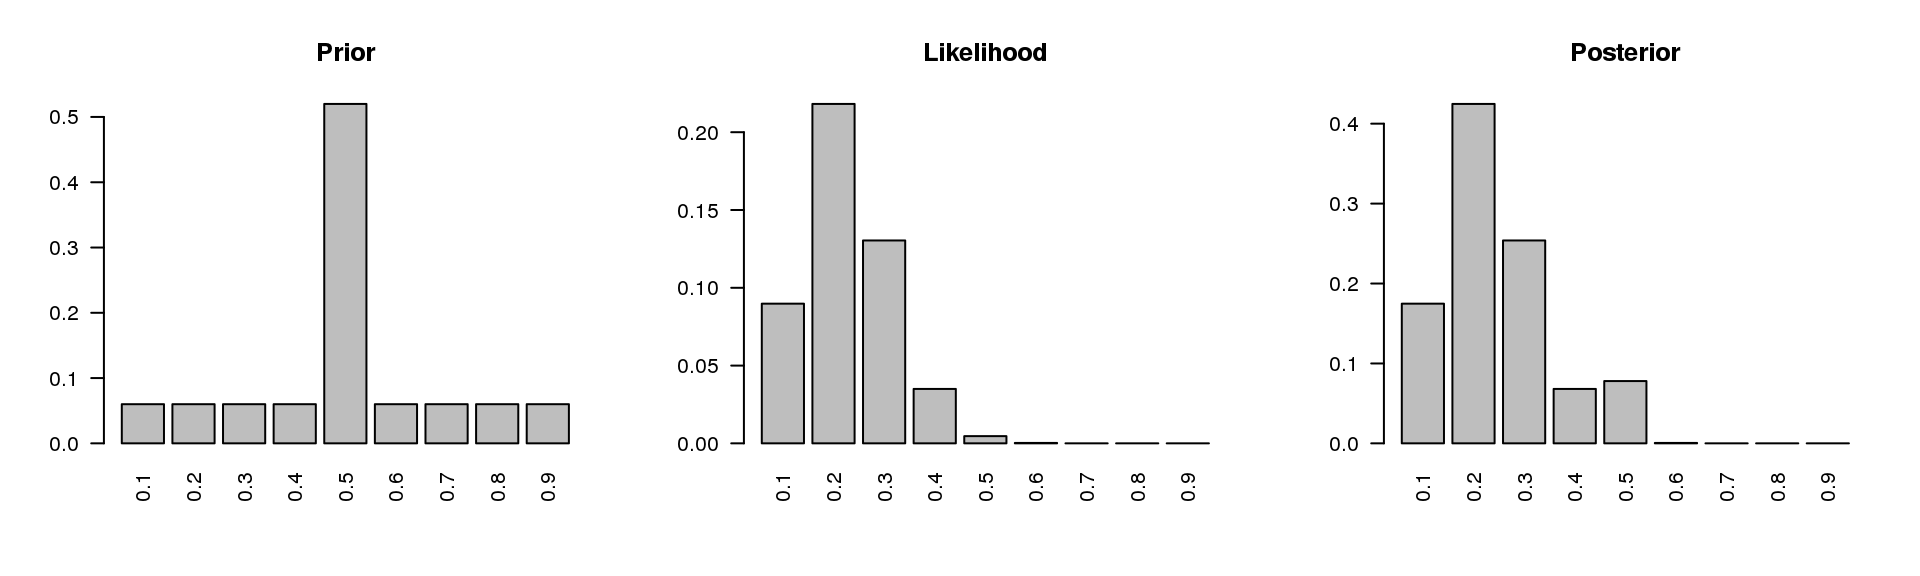
\includegraphics{01-basics-02-inf-for-prop_files/figure-latex/RU-486plot-1.pdf}
\caption{\label{fig:RU-486plot}Original: sample size \(n=20\) and number of
successes \(k=4\)}
\end{figure}

We started with the high prior at \(p=0.5\), but the data likelihood
peaks at \(p=0.2\). And we updated our prior based on observed data to
find the posterior. The Bayesian paradigm, unlike the frequentist
approach, allows us to make direct probability statements about our
models. For example, we can calculate the probability that RU-486, the
treatment, is more effective than the control as the sum of the
posteriors of the models where \(p<0.5\). Adding up the relevant
posterior probabilities in Table \ref{tab:RU-486prior}, we get the
chance that the treatment is more effective than the control is 92.16\%.

\subsection{Effect of Sample Size on the
Posterior}\label{effect-of-sample-size-on-the-posterior}

The RU-486 example is summarized in Figure \ref{fig:RU-486plot}, and
let's look at what the posterior distribution would look like if we had
more data.

\begin{figure}
\centering
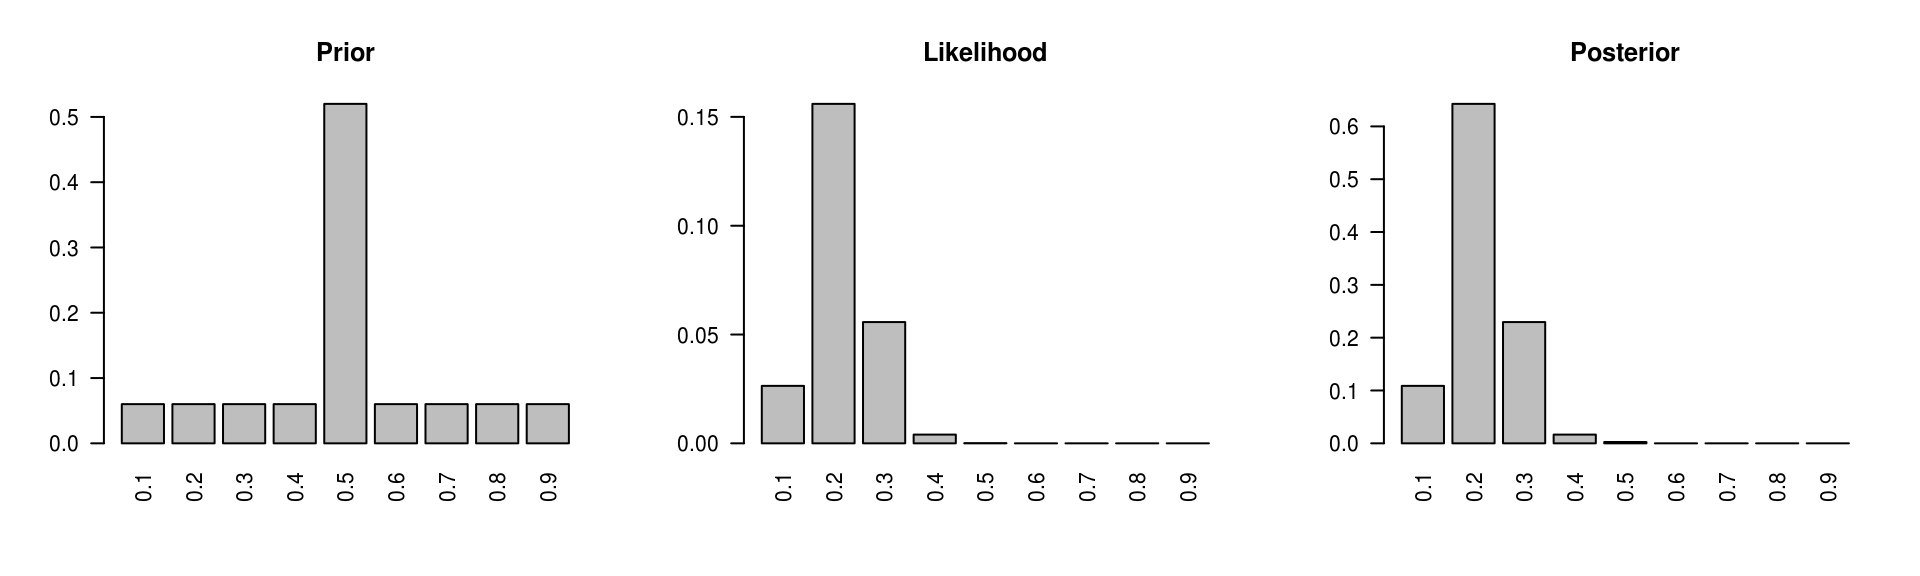
\includegraphics{01-basics-02-inf-for-prop_files/figure-latex/RU-486plotX2-1.pdf}
\caption{\label{fig:RU-486plotX2}More data: sample size \(n=40\) and number
of successes \(k=8\)}
\end{figure}

Suppose our sample size was 40 instead of 20, and the number of
successes was 8 instead of 4. Note that the ratio between the sample
size and the number of successes is still 20\%. We will start with the
same prior distribution. Then calculate the likelihood of the data which
is also centered at 0.20, but is less variable than the original
likelihood we had with the smaller sample size. And finally put these
two together to obtain the posterior distribution. The posterior also
has a peak at p is equal to 0.20, but the peak is taller, as shown in
Figure \ref{fig:RU-486plotX2}. In other words, there is more mass on
that model, and less on the others.

\begin{figure}
\centering
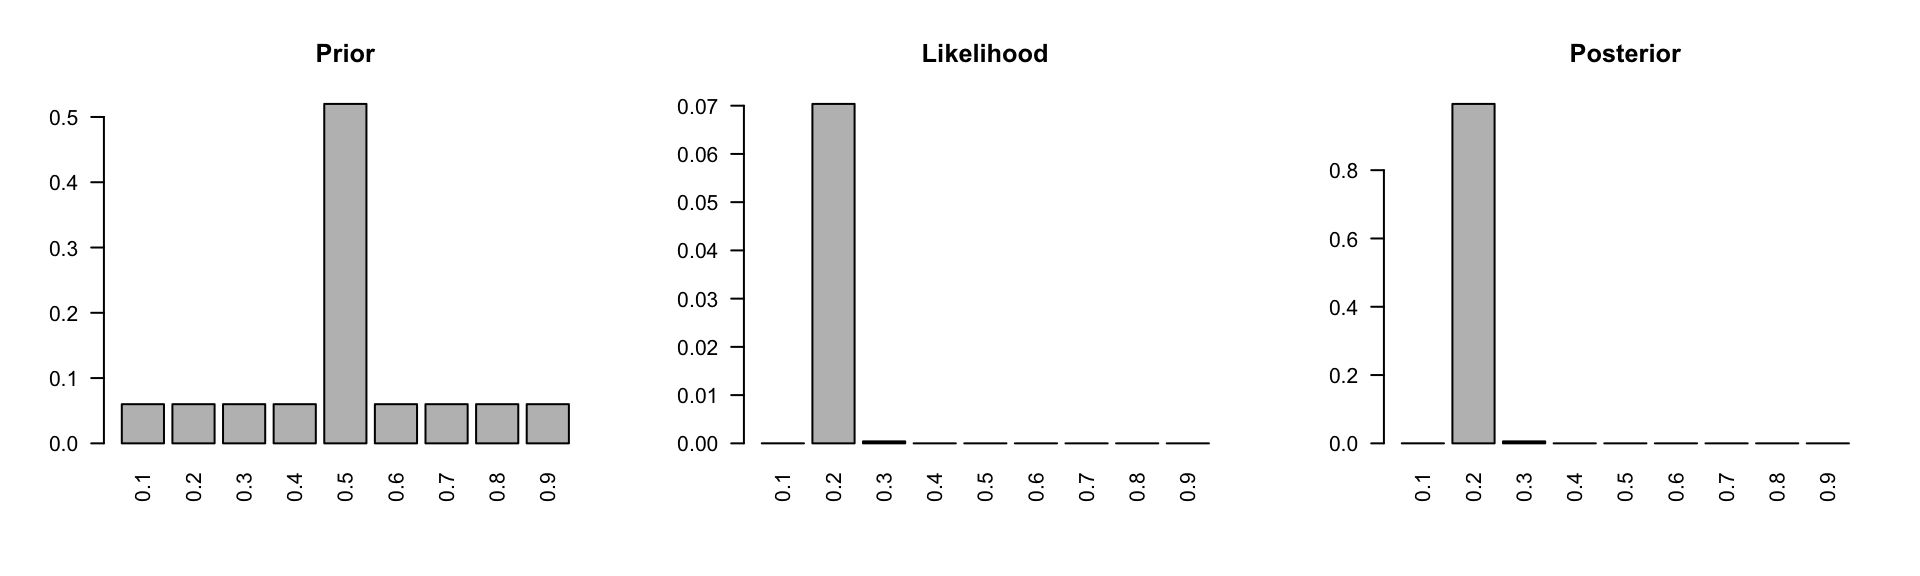
\includegraphics{01-basics-02-inf-for-prop_files/figure-latex/RU-486plotX10-1.pdf}
\caption{\label{fig:RU-486plotX10}More data: sample size \(n=200\) and
number of successes \(k=40\)}
\end{figure}

To illustrate the effect of the sample size even further, we're going to
keep increasing our sample size, but still maintain the the 20\% ratio
between the sample size and the number of successes. So let's consider a
sample with 200 observations and 40 successes. Once again, we're going
to use the same prior and the likelihood is again centered at 20\% and
almost all of the probability mass in the posterior is at p is equal to
0.20. The other models do not have zero probability mass, but they're
posterior probabilities are very close to zero.

Figure \ref{fig:RU-486plotX10} demonstrates that \textbf{as more data
are collected, the likelihood ends up dominating the prior}. This is
why, while a good prior helps, a bad prior can be overcome with a large
sample. However, it's important to note that this will only work as long
as we don't place a zero probability mass on any of the models in the
prior.

\section{Frequentist vs.~Bayesian
Inference}\label{frequentist-vs.bayesian-inference}

\subsection{Frequentist vs.~Bayesian
Inference}\label{frequentist-vs.bayesian-inference-1}

In this section, we will solve a simple inference problem using both
frequentist and Bayesian approaches. Then we will compare our results
based on decisions based on the two methods, to see whether we get the
same answer or not. If we do not, we will discuss why that happens.

\BeginKnitrBlock{example}
\protect\hypertarget{exm:MM}{}{\label{exm:MM} }We have a population of
M\&M's, and in this population the percentage of yellow M\&M's is either
10\% or 20\%. You've been hired as a statistical consultant to decide
whether the true percentage of yellow M\&M's is 10\% or 20\%.

Payoffs/losses: You are being asked to make a decision, and there are
associated payoff/losses that you should consider. If you make the
correct decision, your boss gives you a bonus. On the other hand, if you
make the wrong decision, you lose your job.

Data: You can ``buy'' a random sample from the population -- You pay
\$200 for each M\&M, and you must buy in \$1,000 increments (5 M\&Ms at
a time). You have a total of \$4,000 to spend, i.e., you may buy 5, 10,
15, or 20 M\&Ms.

Remark: Remember that the cost of making a wrong decision is high, so
you want to be fairly confident of your decision. At the same time,
though, data collection is also costly, so you don't want to pay for a
sample larger than you need. If you believe that you could actually make
a correct decision using a smaller sample size, you might choose to do
so and save money and resources.
\EndKnitrBlock{example}

Let's start with the frequentist inference.

\begin{itemize}
\item
  Hypothesis: \(H_0\) is 10\% yellow M\&Ms, and \(H_A\) is
  \textgreater{}10\% yellow M\&Ms.
\item
  Significance level: \(\alpha = 0.05\).
\item
  Sample: red, green, \textbf{yellow}, blue, orange
\item
  Observed data: \(k=1, n=5\)
\item
  P-value:
  \(P(k \geq 1 | n=5, p=0.10) = 1 - P(k=0 | n=5, p=0.10) = 1 - 0.90^5 \approx 0.41\)
\end{itemize}

Note that the p-value is the probability of observed or more extreme
outcome given that the null hypothesis is true.

Therefore, we fail to reject \(H_0\) and conclude that the data do not
provide convincing evidence that the proportion of yellow M\&M's is
greater than 10\%. This means that if we had to pick between 10\% and
20\% for the proportion of M\&M's, even though this hypothesis testing
procedure does not actually confirm the null hypothesis, we would likely
stick with 10\% since we couldn't find evidence that the proportion of
yellow M\&M's is greater than 10\%.

The Bayesian inference works differently as below.

\begin{itemize}
\item
  Hypotheses: \(H_1\) is 10\% yellow M\&Ms, and \(H_2\) is 20\% yellow
  M\&Ms.
\item
  Prior: \(P(H_1) = P(H_2) = 0.5\)
\item
  Sample: red, green, \textbf{yellow}, blue, orange
\item
  Observed data: \(k=1, n=5\)
\item
  Likelihood:
\end{itemize}

\[\begin{aligned}
P(k=1 | H_1) &= \left( \begin{array}{c} 5 \\ 1 \end{array} \right) \times 0.10 \times 0.90^4 \approx 0.33 \\
P(k=1 | H_2) &= \left( \begin{array}{c} 5 \\ 1 \end{array} \right) \times 0.20 \times 0.80^4 \approx 0.41
\end{aligned}\]

\begin{itemize}
\tightlist
\item
  Posterior
\end{itemize}

\[\begin{aligned}
P(H_1 | k=1) &= \frac{P(H_1)P(k=1 | H_1)}{P(k=1)} = \frac{0.5 \times 0.33}{0.5 \times 0.33 + 0.5 \times 0.41} \approx 0.45 \\
P(H_2 | k=1) &= 1 - 0.45 = 0.55
\end{aligned}\]

The posterior probabilities of whether \(H_1\) or \(H_2\) is correct are
close to each other. As a result, with equal priors and a low sample
size, it is difficult to make a decision with a strong confidence, given
the observed data. However, \(H_2\) has a higher posterior probability
than \(H_1\), so if we had to make a decision at this point, we should
pick \(H_2\), i.e., the proportion of yellow M\&Ms is 20\%. Note that
this decision contradicts with the decision based on the frequentist
approach.

Table \ref{tab:freq-vs-bayes} summarizes what the results would look
like if we had chosen larger sample sizes. Under each of these
scenarios, the frequentist method yields a higher p-value than our
significance level, so we would fail to reject the null hypothesis with
any of these samples. On the other hand, the Bayesian method always
yields a higher posterior for the second model where \(p\) is equal to
0.20. So the decisions that we would make are contradictory to each
other.

\begin{table}

\caption{\label{tab:freq-vs-bayes}Frequentist and Bayesian probabilities for larger sample sizes}
\centering
\begin{tabular}[t]{llll}
\toprule
 & Frequentist & Bayesian H\_1 & Bayesian H\_2\\
\midrule
Observed Data & P(k or more | 10\% yellow) & P(10\% yellow | n, k) & P(20\% yellow | n, k)\\
n = 5, k = 1 & 0.41 & 0.45 & 0.55\\
n = 10, k = 2 & 0.26 & 0.39 & 0.61\\
n = 15, k = 3 & 0.18 & 0.34 & 0.66\\
n = 20, k = 4 & 0.13 & 0.29 & 0.71\\
\bottomrule
\end{tabular}
\end{table}

However, if we had set up our framework differently in the frequentist
method and set our null hypothesis to be \(p = 0.20\) and our
alternative to be \(p < 0.20\), we would obtain different results. This
shows that \textbf{the frequentist method is highly sensitive to the
null hypothesis}, while in the Bayesian method, our results would be the
same regardless of which order we evaluate our models.

\section{Exercises}\label{exercises}

\begin{enumerate}
\def\labelenumi{\arabic{enumi}.}
\item
  \textbf{Conditioning on dating site usage.} Recall Table
  \ref{tab:2015gallupDating}. What is the probability that an online
  dating site user from this sample is 18-29 years old?
\item
  \textbf{Probability of no HIV.} Consider the ELISA test from Section
  \ref{sec:diagnostic-testing}. What is the probability that someone has
  no HIV if that person has a negative ELISA result? How does this
  compare to the probability of having no HIV before any test was done?
\item
  \textbf{Probability of no HIV after contradictive tests.} Consider the
  ELISA test from Section \ref{sec:diagnostic-testing}. What is the
  probability that someone has no HIV if that person first tests
  positive on the ELISA and secondly test negative? Assume that the
  tests are independent from each other.
\end{enumerate}

\chapter{Bayesian Inference}\label{bayesian-inference}

This chapter is focused on the continuous version of Bayes' rule and how
to use it in a conjugate family. The RU-486 example will allow us to
discuss Bayesian modeling in a concrete way. It also leads naturally to
a Bayesian analysis without conjugacy. For the non-conjugate case,
there's usually no simple mathematical expression, and one must resort
to computation. Finally, we discuss credible intervals, i.e., the
Bayesian analog of frequentist confidence intervals, and Bayesian
estimation and prediction.

It is assumed that the readers have mastered the concept of conditional
probability and the Bayes' rule for discrete random variables. Calculus
is not required for this chapter; however, for those who do, we shall
briefly look at an integral.

\section{Continuous Variables and Eliciting Probability
Distributions}\label{continuous-variables-and-eliciting-probability-distributions}

\subsection{From the Discrete to the
Continuous}\label{from-the-discrete-to-the-continuous}

This section leads the reader from the discrete random variable to
continuous random variables. Let's start with the binomial random
variable such as the number of heads in ten coin tosses, can only take a
discrete number of values -- 0, 1, 2, up to 10.

When the probability of a coin landing heads is \(p\), the chance of
getting \(k\) heads in \(n\) tosses is

\[P(X = k) = \left( \begin{array}{c} n \\ k \end{array} \right) p^k (1-p)^{n-k}\].

This formula is called the \textbf{probability mass function} (pmf) for
the binomial.

The probability mass function can be visualized as a histogram in Figure
\ref{fig:histogram}. The area under the histogram is one, and the area
of each bar is the probability of seeing a binomial random variable,
whose value is equal to the x-value at the center of the bars base.

\begin{figure}

{\centering 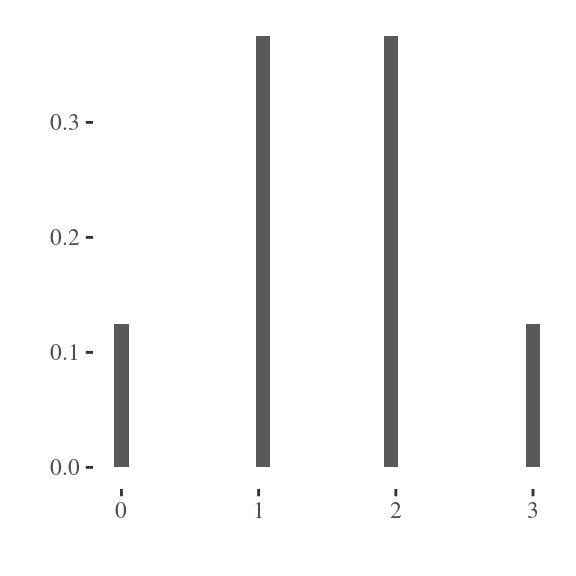
\includegraphics{02-inference-01-continuous_files/figure-latex/histogram-1} 

}

\caption{Histogram of binomial random variable}\label{fig:histogram}
\end{figure}

In contrast, the normal distribution, a.k.a. Gaussian distribution or
the bell-shaped curve, can take any numerical value in
\((-\infty,+\infty)\). A random variable generated from a normal
distribution because it can take a continuum of values.

In general, if the set of possible values a random variable can take are
separated points, it is a discrete random variable. But if it can take
any value in some (possibly infinite) interval, then it is a continuous
random variable.

When the random variable is \textbf{discrete}, it has a
\textbf{probability mass function} or pmf. That pmf tells us the
probability that the random variable takes each of the possible values.
But when the random variable is continuous, it has probability zero of
taking any single value. (Hence probability zero does not equal to
impossible, an event of probabilty zero can still happen.)

We can only talk about the probability of a continuous random variable
lined within some interval. For example, suppose that heights are
approximately normally distributed. The probability of finding someone
who is exactly 6 feet tall at 0.0000 inches tall for an infinite number
of 0s after the decimal point is 0. But we can easily calculate the
probability of finding someone who is between 5'11" inches tall and 6'1"
inches tall.

A \textbf{continuous} random variable has a \textbf{probability density
function} or pdf, instead of probability mass functions. The probability
of finding someone whose height lies between 5'11" (71 inches) and 6'1"
(73 inches) is the area under the pdf curve for height between those two
values, as shown in the blue area of Figure \ref{fig:pdf-auc}.\footnote{Code
  reference: \url{http://www.statmethods.net/advgraphs/probability.html}}

\begin{figure}

{\centering 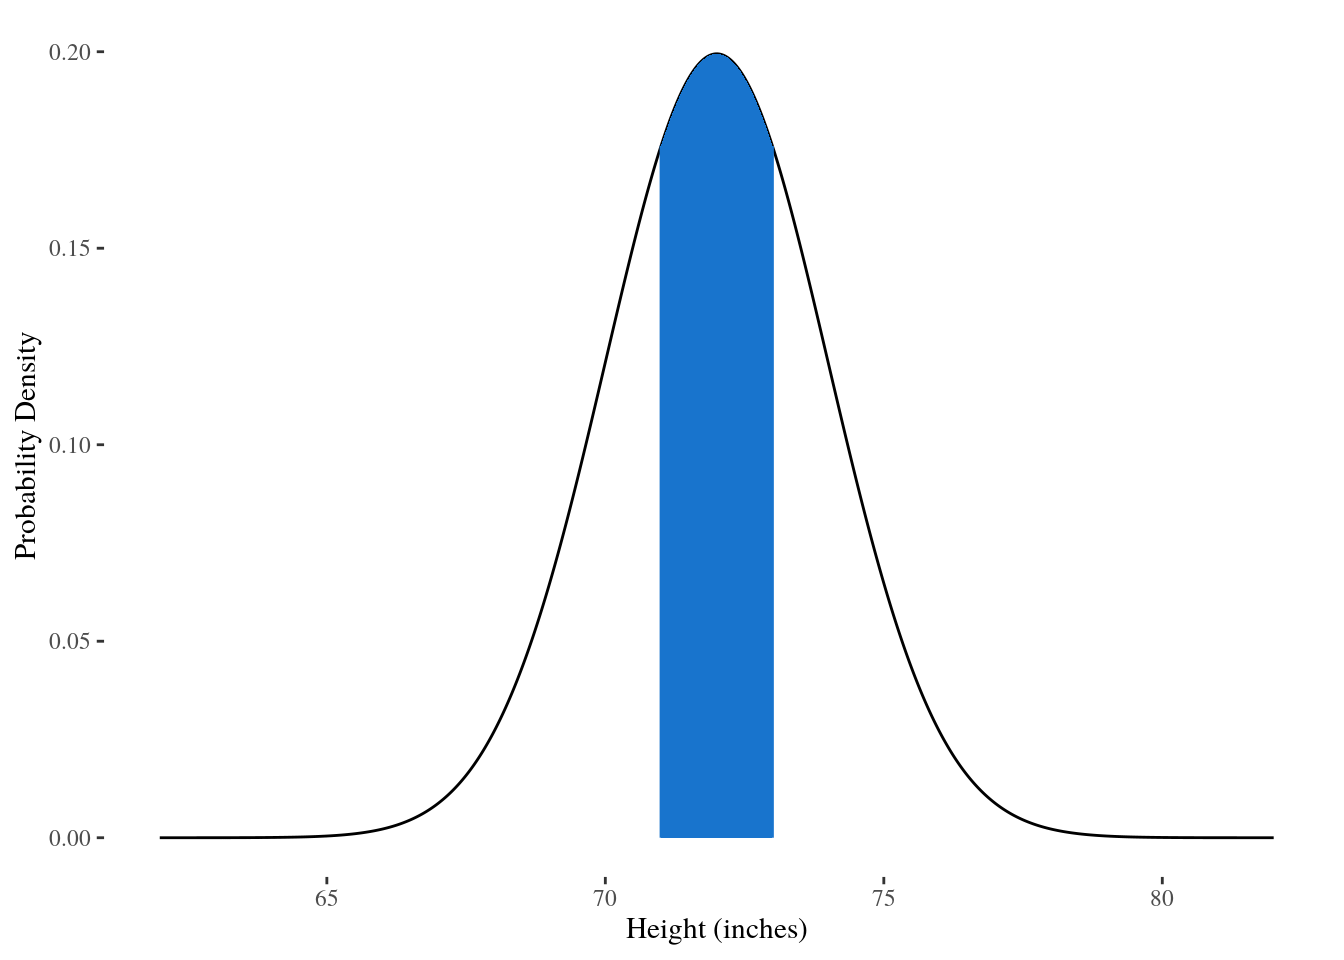
\includegraphics{02-inference-01-continuous_files/figure-latex/pdf-auc-1} 

}

\caption{Area under curve for the probability density function}\label{fig:pdf-auc}
\end{figure}

For example, a normal distribution with mean \(\mu\) and standard
deviation \(\sigma\) (i.e., variance \(\sigma^2\)) is defined as

\[f(x) = \frac{1}{\sqrt{2 \pi \sigma^2}} \exp[-\frac{1}{2\sigma^2}(x-\mu)^2],\]

where \(x\) is any value the random variable \(X\) can take. This is
denoted as \(X \sim N(\mu,\sigma^2)\), where \(\mu\) and \(\sigma^2\)
are the parameters of the normal distribution.

Recall that a probability mass function assigns the probability that a
random variable takes a specific value for the discrete set of possible
values. The sum of those probabilities over all possible values must
equal one.

Similarly, a probability density function is any \(f(x)\) that is
non-negative and has area one underneath its curve. The pdf can be
regarded as the limit of histograms made from its sample data. As the
sample size becomes infinitely large, the bin width of the histogram
shrinks to zero.

There are infinite number of pmf's and an infinite number of pdf's. Some
distributions are so important that they have been given names:

\begin{itemize}
\item
  Continuous: normal, uniform, beta, gamma
\item
  Discrete: binomial, Poisson
\end{itemize}

Here is a summary of the key ideas in this section:

\begin{enumerate}
\def\labelenumi{\arabic{enumi}.}
\item
  Continuous random variables exist and they can take any value within
  some possibly infinite range.
\item
  The probability that a continuous random variable takes a specific
  value is zero.
\item
  Probabilities from a continuous random variable are determined by the
  density function with this non-negative and the area beneath it is
  one.
\item
  We can find the probability that a random variable lies between two
  values (\(c\) and \(d\)) as the area under the density function that
  lies between them.
\end{enumerate}

\subsection{Elicitation}\label{elicitation}

Next, we introduce the concept of prior elicitation in base and
statistics. Often, one has a belief about the distribution of one's
data. You may think that your data come from a binomial distribution and
in that case you typically know the \(n\), the number of trials but you
usually do not know \(p\), the probability of success. Or you may think
that your data come from a normal distribution. But you do not know the
mean \(\mu\) or the standard deviation \(\sigma\) of the normal. Beside
to knowing the distribution of one's data, you may also have beliefs
about the unknown \(p\) in the binomial or the unknown mean \(\mu\) in
the normal.

Bayesians express their belief in terms of personal probabilities. These
personal probabilities encapsulate everything a Bayesian knows or
believes about the problem. But these beliefs must obey the laws of
probability, and be consistent with everything else the Bayesian knows.

\BeginKnitrBlock{example}
\protect\hypertarget{exm:200percent}{}{\label{exm:200percent} }You cannot
say that your probability of passing this course is 200\%, no matter how
confident you are. A probability value must be between zero and one. (If
you still think you have a probability of 200\% to pass the course, you
are definitely not going to pass it.)
\EndKnitrBlock{example}

\BeginKnitrBlock{example}
\protect\hypertarget{exm:binomial-data}{}{\label{exm:binomial-data} }You may
know nothing at all about the value of \(p\) that generated some
binomial data. In which case any value between zero and one is equally
likely, you may want to make an inference on the proportion of people
who would buy a new band of toothpaste. If you have industry experience,
you may have a strong belief about the value of \(p\), but if you are
new to the industry you would do nothing about \(p\). In any value
between zero and one seems equally like a deal. This major personal
probability is the uniform distribution whose probably density function
is flat, denoted as \(\text{Unif}(0,1)\).
\EndKnitrBlock{example}

\BeginKnitrBlock{example}
\protect\hypertarget{exm:coin-toss}{}{\label{exm:coin-toss} }If you were
tossing a coin, most people believed that the probability of heads is
pretty close to half. They know that some coin are loaded and they know
that some coins may have two heads or two tails. And they probably also
know that coins are not perfectly balanced. Nonetheless, before they
start to collect data by tossing the coin and counting the number of
heads their belief is that values of \(p\) near 0.5 are very likely,
where's values of \(p\) near 0 or 1 are very unlikely.
\EndKnitrBlock{example}

\BeginKnitrBlock{example}
\protect\hypertarget{exm:marriage}{}{\label{exm:marriage} }In real life,
here are two ways to elicit a probability that you cousin will get
married. A frequentist might go to the U.S. Census records and determine
what proportion of people get married (or, better, what proportion of
people of your cousin's ethnicity, education level, religion, and age
cohort are married). In contrast, a Bayesian might think ``My cousin is
brilliant, attractive, and fun. The probability that my cousin gets
married is really high -- probably around 0.97.''
\EndKnitrBlock{example}

So a base angle sits to express their belief about the value of \(p\)
through a probability distribution, and a very flexible family of
distributions for this purpose is the \textbf{beta family}. A member of
the beta family is specified by two parameters, \(\alpha\) and
\(\beta\); we denote this as \(p \sim \text{beta}(\alpha, \beta)\). The
probability density function is

\begin{equation}
f(p) = \frac{\Gamma(\alpha+\beta)}{\Gamma(\alpha)\Gamma(\beta)} p^{\alpha-1} (1-p)^{\beta-1},
\label{eq:beta}
\end{equation}

where \(0 \leq p \leq 1, \alpha>0, \beta>0\), and \(\Gamma\) is a
factorial:

\[\Gamma(n) = (n-1)! = (n-1) \times (n-2) \times \cdots \times 1\]

When \(\alpha=\beta=1\), the beta distribution becomes a uniform
distribution, i.e.~the probabilty density function is a flat line. In
other words, the uniform distribution is a special case of the beta
family.

The expected value of \(p\) is \(\frac{\alpha}{\alpha+\beta}\), so
\(\alpha\) can be regarded as the prior number of successes, and
\(\beta\) the prior number of failures. When \(\alpha=\beta\), then one
gets a symmetrical pdf around 0.5. For large but equal values of
\(\alpha\) and \(\beta\), the area under the beta probability density
near 0.5 is very large. Figure \ref{fig:beta} compares the beta
distribution with different parameter values.

\begin{figure}

{\centering 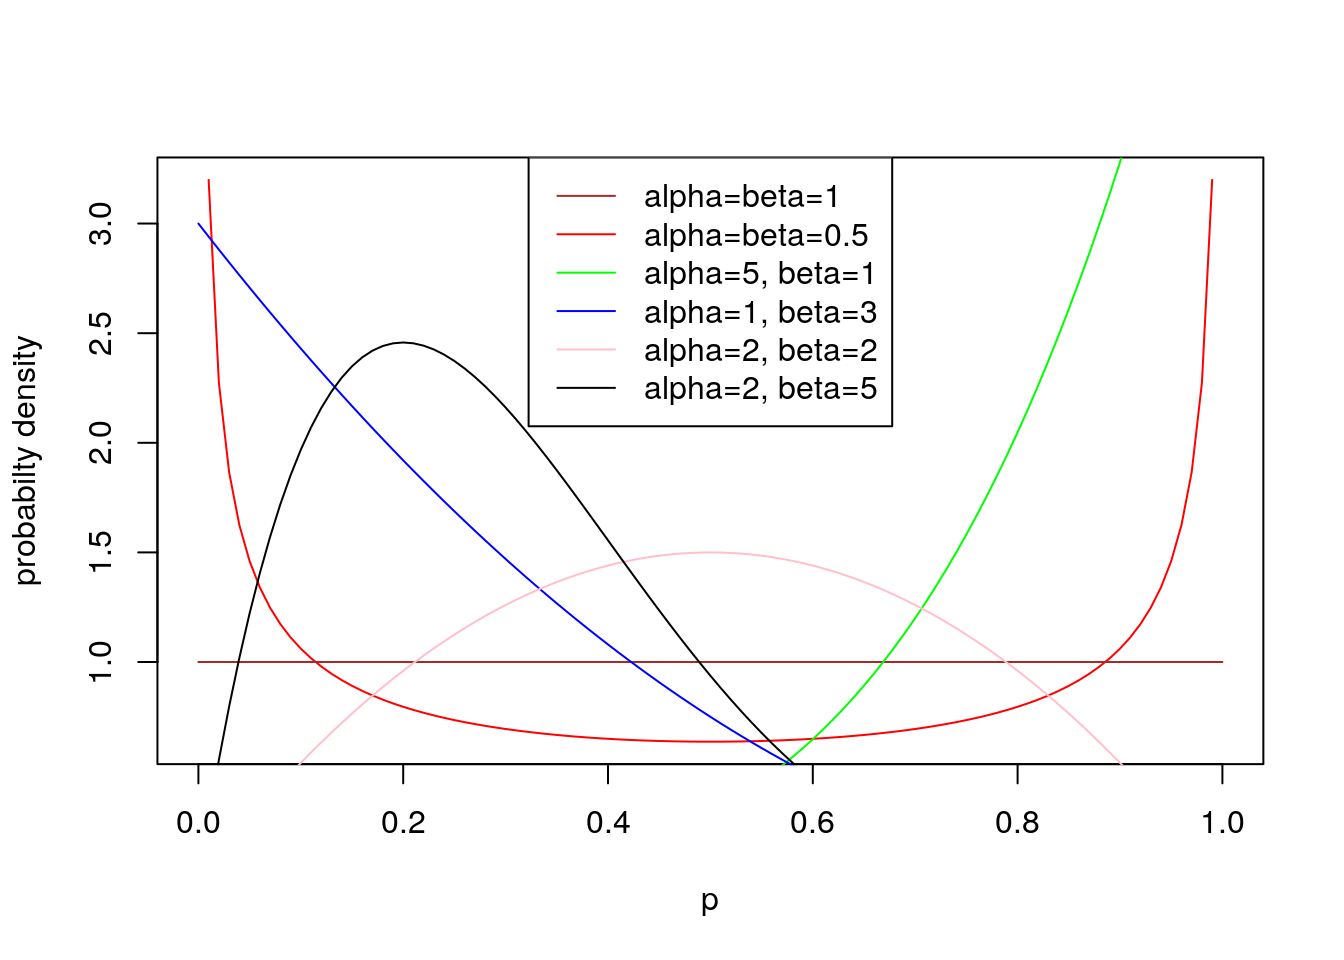
\includegraphics{02-inference-01-continuous_files/figure-latex/beta-1} 

}

\caption{Beta family}\label{fig:beta}
\end{figure}

These kinds of priors are probably appropriate if you want to infer the
probability of getting heads in a coin toss. The beta family also
includes skewed densities, which is appropriate if you think that \(p\)
the probability of success in ths binomial trial is close to zero or
one.

Bayes' rule is a machine to turn one's prior beliefs into posterior
beliefs. With binomial data you start with whatever beliefs you may have
about \(p\), then you observe data in the form of the number of head,
say 20 tosses of a coin with 15 heads.

Next, Bayes' rule tells you how the data changes your opinion about
\(p\). The same principle applies to all other inferences. You start
with your prior probability distribution over some parameter, then you
use data to update that distribution to become the posterior
distribution that expresses your new belief.

These rules ensure that the change in distributions from prior to
posterior is the uniquely rational solution. So, as long as you begin
with the prior distribution that reflects your true opinion, you can
hardly go wrong.

However, expressing that prior can be difficult. There are proofs and
methods whereby a rational and coherent thinker can self-illicit their
true prior distribution, but these are impractical and people are rarely
rational and coherent.

The good news is that with the few simple conditions no matter what part
distribution you choose. If enough data are observed, you will converge
to an accurate posterior distribution. So, two bayesians, say the
reference Thomas Bayes and the agnostic Ajay Good can start with
different priors but, observe the same data. As the amount of data
increases, they will converge to the same posterior distribution.

Here is a summary of the key ideas in this section:

\begin{enumerate}
\def\labelenumi{\arabic{enumi}.}
\item
  Bayesians express their uncertainty through probability distributions.
\item
  One can think about the situation and self-elicit a probability
  distribution that approximately reflects his/her personal probability.
\item
  One's personal probability should change according Bayes' rule, as new
  data are observed.
\item
  The beta family of distribution can describe a wide range of prior
  beliefs.
\end{enumerate}

\subsection{Conjugacy}\label{conjugacy}

Next, let's introduce the concept of conjugacy in Bayesian statistics.

Suppose we have the prior beliefs about the data as below:

\begin{itemize}
\item
  Binomial distribution \(\text{Bin}(n,p)\) with \(n\) known and \(p\)
  unknown
\item
  Prior belief about \(p\) is \(\text{beta}(\alpha,\beta)\)
\end{itemize}

Then we observe \(x\) success in \(n\) trials, and it turns out the
Bayes' rule implies that our new belief about the probability density of
\(p\) is also the beta distribution, but with different parameters. In
mathematical terms,

\begin{equation}
p|x \sim \text{beta}(\alpha+x, \beta+n-x).
\label{eq:beta-binomial}
\end{equation}

This is an example of conjugacy. Conjugacy occurs when the
\textbf{posterior distribution} is in the \textbf{same family} of
probability density functions as the prior belief, but with \textbf{new
parameter values}, which have been updated to reflect what we have
learned from the data.

Why are the beta binomial families conjugate? Here is a mathematical
explanation.

Recall the discrete form of the Bayes' rule:

\[P(A_i|B) = \frac{P(B|A_i)P(A_i)}{\sum^n_{j=1}P(B|A_j)P(A_j)}\]

However, this formula does not apply to continuous random variables,
such as the \(p\) which follows a beta distribution, because the
denominator sums over all possible values (must be finitely many) of the
random variable.

But the good news is that the \(p\) has a finite range -- it can tak any
value \textbf{only} between 0 and 1. Hence we can perform integration,
which is a generalization of the summation. The Bayes' rule can also be
written in continuous form as:

\[\pi^*(p|x) = \frac{P(x|p)\pi(p)}{\int^1_0 P(x|p)\pi(p) dp}.\]

This is analogus to the discrete form, since the integral in the
denominator will also be equal to some constant, just like a summation.
This constant ensures that the total area under the curve, i.e.~the
posterior density function, equals 1.

Note that in the numerator, the first term, \(P(x|p)\), is the data
likelihood -- the probability of observing the data given a specific
value of \(p\). The second term, \(\pi(p)\), is the probability density
function that reflects the prior belief about \(p\).

In the beta-binomial case, we have \(P(x|p)=\text{Bin}(n,p)\) and
\(\pi(p)=\text{beta}(\alpha,\beta)\).

Plugging in these distributions, we get

\[\begin{aligned}
\pi^*(p|x) &= \frac{1}{\text{some number}} \times P(x|p)\pi(p) \\
&= \frac{1}{\text{some number}} [\left( \begin{array}{c} n \\ x \end{array} \right) p^x (1-p)^{n-x}] [\frac{\Gamma(\alpha+\beta)}{\Gamma(\alpha)\Gamma(\beta)} p^{\alpha-1} (1-p)^{\beta-1}] \\
&= \frac{\Gamma(\alpha+\beta+n)}{\Gamma(\alpha+x)\Gamma(\beta+n-x)} \times p^{\alpha+x-1} (1-p)^{\beta+n-x-1}
\end{aligned}\]

Let \(\alpha^* = \alpha + x\) and \(\beta^* = \beta+n-x\), and we get

\[\pi^*(p|x) = \text{beta}(\alpha^*,\beta^*) = \text{beta}(\alpha+x, \beta+n-x),\]

same as the posterior formula in Equation \eqref{eq:beta-binomial}.

We can recognize the posterior distribution from the numerator
\(p^{\alpha+x-1}\) and \((1-p)^{\beta+n-x-1}\). Everything else are just
constants, and they must take the unique value, which is needed to
ensure that the area under the curve between 0 and 1 equals 1. So they
have to take the values of the beta, which has parameters \(\alpha+x\)
and \(\beta+n-x\).

This is a cute trick. We can find the answer without doing the integral
simply by looking at form of the numerator.

Without conjugacy, one has to do the integral. Often, the integral is
impossible to evaluate. That obstacle is the primary reason that most
statistical theory in the 20th century was not Bayesian. The situation
didn't change until modern computing allowed researchers to compute
integrals numerically.

In summary, some pairs of distributions are conjugate. If your prior is
in one and your data comes from the other, then your posterior is in the
same family as the prior, but with new parameters. We explored this in
the context of the beta-binomial conjugate families. And we saw that
conjugacy meant that we could apply the continuous version of Bayes'
rule without having to do any integration.

\section{Three Conjugate Families}\label{three-conjugate-families}

In this section, the three conjugate families are beta-binomial,
normal-gamma, and normal-normal pairs. Each of them has its own
applications in everyday life.

\subsection{Inference on a Binomial
Proportion}\label{inference-on-a-binomial-proportion}

\BeginKnitrBlock{example}
\protect\hypertarget{exm:RU-486more}{}{\label{exm:RU-486more} }Recall
Example \ref{exm:RU-486}, a simplified version of a real clinical trial
taken in Scotland. It concerned RU-486, a morning after pill that was
being studied to determine whether it was effective at preventing
unwanted pregnancies. It had 800 women, each of whom had intercourse no
more than 72 hours before reporting to a family planning clinic to seek
contraception.

Half of these women were randomly assigned to the standard
contraceptive, a large dose of estrogen and progesterone. And half of
the women were assigned RU-486. Among the RU-486 group, there were no
pregnancies. Among those receiving the standard therapy, four became
pregnant.
\EndKnitrBlock{example}

Statistically, one can model these data as coming from a binomial
distribution. Imagine a coin with two sides. One side is labeled
standard therapy and the other is labeled RU-486. The coin was tossed
four times, and each time it landed with the standard therapy side face
up.

A frequentist would analyze the problem as below:

\begin{itemize}
\item
  The parameter \(p\) is the probability of a preganancy comes from the
  standard treatment.
\item
  \(H_0: p \geq 0.5\) and \(H_A: p < 0.5\)
\item
  The p-value is \(0.5^4 = 0.0625 > 0.05\)
\end{itemize}

Therefore, the frequentist fails to reject the null hypothesis, and will
not conclude that RU-486 is superior to standard therapy.

Remark: The significance probability, or p-value, is the chance of
observing data that are as or more supportive of the alternative
hypothesis than the data that were collected, when the null hypothesis
is true.

Now suppose a Bayesian performed the analysis. She may set her beliefs
about the drug and decide that she has no prior knowledge about the
efficacy of RU-486 at all. This would be reasonable if, for example, it
were the first clinical trial of the drug. In that case, she would be
using the uniform distribution on the interval from 0 to 1, which
corresponds to the \(\text{beta}(1,1)\) density. In mathematical terms,

\[p \sim \text{Unif}(0,1) = \text{beta}(1,1).\]

From conjugacy, we know that since there were four failures for RU-486
and no successes, that her posterior probability of an RU-486 child is

\[p|x \sim \text{beta}(1+0,1+4) = \text{beta}(1,5).\]

This is a beta that has much more area near \(p\) equal to 0. The mean
of \(\text{beta}(\alpha,\beta)\) is \(\frac{\alpha}{\alpha+\beta}\). So
this Bayesian now believes that the unknown \(p\), the probability of an
RU-468 child, is about 1 over 6.

The standard deviation of a beta distribution with parameters in alpha
and beta also has a closed form:

\[p \sim \text{beta}(\alpha,\beta) \Rightarrow \text{Standard deviation} = \sqrt{\frac{\alpha\beta}{(\alpha+\beta)^2(\alpha+\beta+1)}}\]

Before she saw the data, the Bayesian's uncertainty expressed by her
standard deviation was 0.71. After seeing the data, it was much reduced
-- her posterior standard deviation is just 0.13.

We promised not to do much calculus, so I hope you will trust me to tell
you that this Bayesian now believes that her posterior probability that
\(p < 0.5\) is 0.96875. She thought there was a 50-50 chance that RU-486
is better. But now she thinks there's about a 97\% chance that RU-486 is
better.

Suppose a fifth child were born, also to a mother who received standard
chip therapy. Now the Bayesian's prior is beta(1, 5) and the additional
data point further updates her to a new posterior beta of 1 and 6.
\textbf{As data comes in, the Bayesian's previous posterior becomes her
new prior, so learning is self-consistent.}

This example has taught us several things:

\begin{enumerate}
\def\labelenumi{\arabic{enumi}.}
\item
  We saw how to build a statistical model for an applied problem.
\item
  We could compare the frequentist and Bayesian approaches to inference
  and see large differences in the conclusions.
\item
  We saw how the data changed the Bayesian's opinion with a new mean for
  p and less uncertainty.
\item
  We learned that Bayesian's continually update as new data arrive.
  \textbf{Yesterday's posterior is today's prior.}
\end{enumerate}

\subsection{The Gamma-Poisson Conjugate
Families}\label{the-gamma-poisson-conjugate-families}

A second important case is the gamma-Poisson conjugate families. In this
case the data come from a Poisson distribution, and the prior and
posterior are both gamma distributions.

The Poisson random variable can take any \textbf{non-negative integer
value} all the way up to infinity. It is used in describing
\textbf{count data}, where one counts the number of independent events
that occur in a fixed amount of time, a fixed area, or a fixed volume.

Moreover, the Poisson distribution has been used to describe the number
of phone calls one receives in an hour. Or, the number of pediatric
cancer cases in the city, for example, to see if pollution has elevated
the cancer rate above that of in previous years or for similar cities.
It is also used in medical screening for diseases, such as HIV, where
one can count the number of T-cells in the tissue sample.

The Poisson distribution has a single parameter \(\lambda\), and it is
denoted as \(X \sim \text{Pois}(\lambda)\) with \(\lambda>0\). The
probability mass function is

\[P(X=k) = \frac{\lambda^k}{k!} \exp^{-\lambda} \text{ for } k=0,1,\cdots,\]

where \(k! = k \times (k-1) \times \cdots \times 1\). This gives the
probability of observing a random variable equal to \(k\).

Note that \(\lambda\) is both the mean and the variance of the Poisson
random variable. It is obvious that \(\lambda\) must be greater than
zero, because it represents the mean number of counts, and the variance
should be greater than zero (except for constants, which have zero
variance).

\BeginKnitrBlock{example}
\protect\hypertarget{exm:Poisson}{}{\label{exm:Poisson} }Famously, von
Bortkiewicz used the Poisson distribution to study the number of
Prussian cavalrymen who were kicked to death by a horse each year. This
is count data over the course of a year, and the events are probably
independent, so the Poisson model makes sense.

He had data on 15 cavalry units for the 20 years between 1875 and 1894,
inclusive. The total number of cavalrymen who died by horse kick was
200.

One can imagine that a Prussian general might want to estimate
\(\lambda\). The average number per year, per unit. Perhaps in order to
see whether some educational campaign about best practices for equine
safety would make a difference.
\EndKnitrBlock{example}

Suppose the Prussian general is a Bayesian. Introspective elicitation
leads him to think that \(\lambda=0.75\) and standard deviation 1.

Modern computing was unavailable at that time yet, so the general will
need to express his prior as a member of a family conjugate to the
Poisson. It turns out that this family consists of the gamma
distributions. Gamma distributions describe continuous non-negative
random variables. As we know, the value of \(\lambda\) in the Poisson
can take any non-negative value so this fits.

The gamma family is flexible, and Figure \ref{fig:gamma} illustrates a
wide range of gamma shapes.

\begin{figure}

{\centering 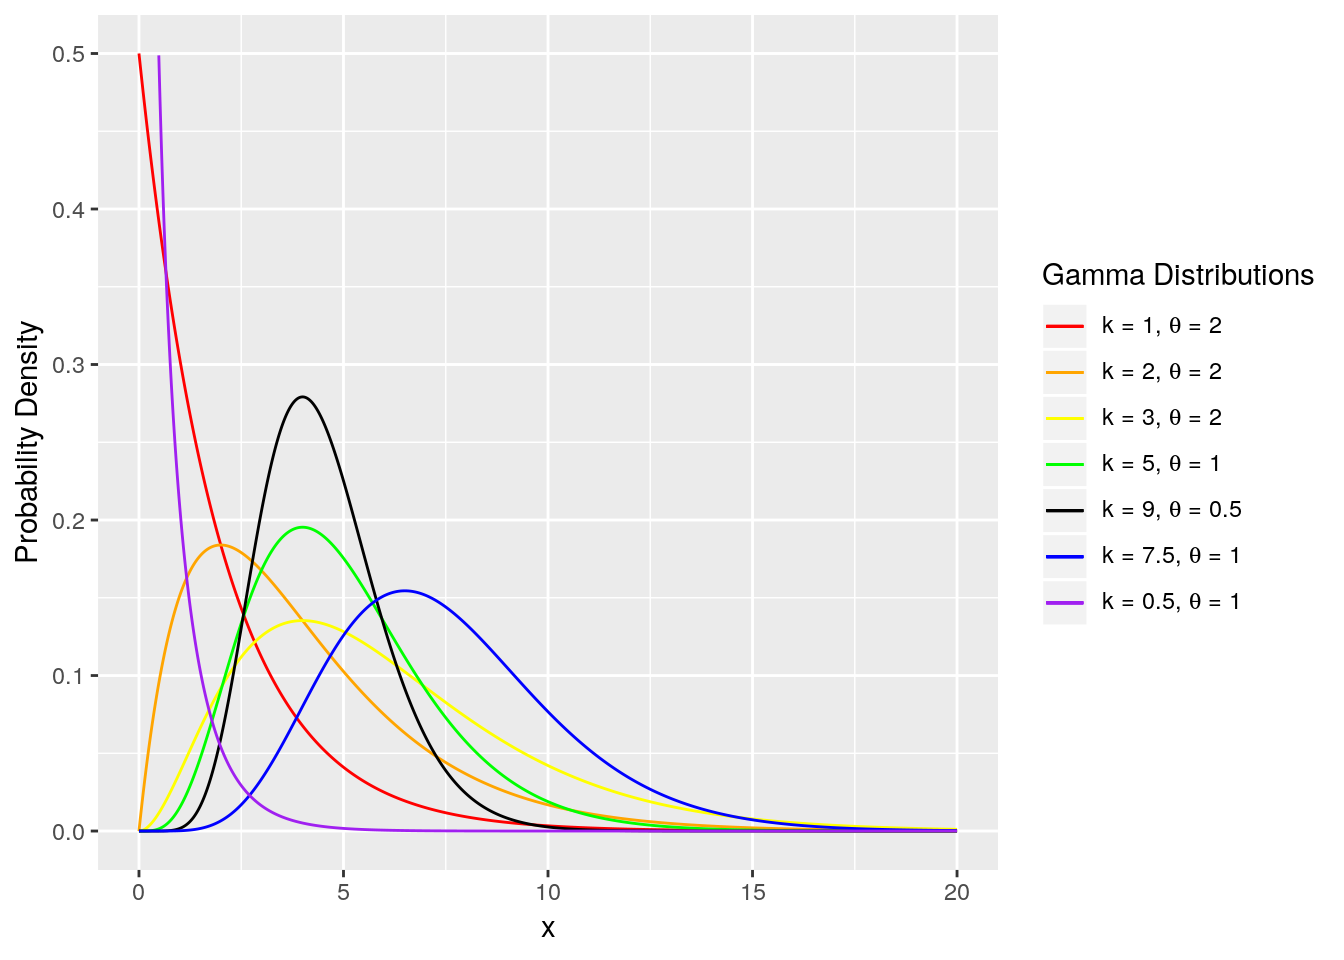
\includegraphics{02-inference-02-conjugate_files/figure-latex/gamma-1} 

}

\caption{Gamma family}\label{fig:gamma}
\end{figure}

The probability density function for the gamma is indexed by shape \(k\)
and scale \(\theta\), denoted as \(\text{Gamma}(k,\theta)\) with
\(k,\theta > 0\). The mathematical form of the distribution is

\[f(x) = \dfrac{1}{\Gamma(k)\theta^k} x^{k-1} e^{-x/\theta},\] where

\[\Gamma(z) = \int^{\infty}_0 x^{z-1} e^{-x} dx.\]

\(\Gamma(z)\), the gamma function, is simply a constant that ensures the
area under curve between 0 and 1 sums to 1, just like in the beta
probability distribution case of Equation \eqref{eq:beta}. A special case
is that \(\Gamma(n) = (n-1)!\) when \(n\) is a positive integer.

However, some books parameterize the gamma distribution in a slightly
different way with shape \(\alpha = k\) and rate (inverse scale)
\(\beta=1/\theta\):

\[f(x) = \frac{\beta^{\alpha}}{\Gamma(\alpha)} x^{\alpha-1} e^{-\beta x}\]

For this example, we use the \(k\)-\(\theta\) parameterization, but you
should always check which parameterization is being used. For example,
\(\mathsf{R}\) uses the \(\alpha\)-\(\beta\) parameterization by
default.\\
In the the later material we find that using the rate parameterization
is more convenient.

** ANY WAY TO MAKE THE MATERIAL MORE IN SYNC AS LABS LATER SECTIONS ALL
USE THE RATE PARAMETERIZATION **

For our parameterization, the mean of \(\text{Gamma}(k,\theta)\) is
\(k\theta\), and the variance is \(k\theta^2\). We can get the general's
prior as below:

\[\begin{aligned}
\text{Mean} &= k\theta = 0.75 \\
\text{Standard deviation} &= \theta\sqrt{k} = 1
\end{aligned}\]

Hence \[k = \frac{9}{16} \text{ and } \theta = \frac{4}{3}\]

For the gamma Poisson conjugate family, suppose we observed data
\(x_1, x_2, \cdots, x_n\) that follow a Poisson distribution.Then
similar to the previous section, we would recognize the kernel of the
gamma when using the gamma-Poisson family. The posterior
\(\text{Gamma}(k^*, \theta^*)\) has parameters

\[k^* = k + \sum^n_{i=1} x_i \text{ and } \theta^* = \frac{\theta}{(n\theta+1)}.\]

For this dataset, \(N = 15 \times 20 = 300\) observations, and the
number of casualities is 200. Therefore, the general now thinks that the
average number of Prussian cavalry officers who die at the hoofs of
their horses follows a gamma distribution with the parameters below:

\[\begin{aligned}
k^* &= k + \sum^n_{i=1} x_i = \frac{9}{16} + 200 = 200.5625 \\
\theta^* = \frac{\theta}{(n\theta+1)} &= \frac{4/3}{300\times(4/3)} = 0.0033
\end{aligned}\]

How the general has changed his mind is described in Table
\ref{tab:before-after}. After seeing the data, his uncertainty about
lambda, expressed as a standard deviation, shrunk from 1 to 0.047.

\begin{table}

\caption{\label{tab:before-after}Before and after seeing the data}
\centering
\begin{tabular}[t]{lrr}
\toprule
  & lambda & Standard Deviation\\
\midrule
Before & 0.75 & 1.000\\
After & 0.67 & 0.047\\
\bottomrule
\end{tabular}
\end{table}

In summary, we learned about the Poisson and gamma distributions; we
also knew that the gamma-Poisson families are conjugate. Moreover, we
learned the updating fomula, and applied it to a classical dataset.

\subsection{The Normal-Normal Conjugate
Families}\label{sec:normal-normal}

There are other conjugate families, and one is the normal-normal pair.
If your data come from a normal distribution with known standard
deviation \(\sigma\) but unknown mean \(\mu\), and if your prior on the
mean \(\mu\), has a normal distribution with self-elicited mean \(\nu\)
and self-elicited standard deviation \(\tau\), then your posterior
density for the mean, after seeing a sample of size \(n\) with sample
mean \(\bar{x}\), is also normal. In mathematical notation, we have

\[\begin{aligned}
x|\mu &\sim N(\mu,\sigma) \\
\mu &\sim N(\nu, \tau)
\end{aligned}\]

As a practical matter, one often does not know sigma, the standard
deviation of the normal from which the data come. In that case, you
could use a more advanced conjugate family that we will describe in
\ref{sec:normal-gamma}. But there are cases in which it is reasonable to
treat the \(\sigma\) as known.

\BeginKnitrBlock{example}
\protect\hypertarget{exm:chemist}{}{\label{exm:chemist} }An analytical
chemist whose balance produces measurements that are normally
distributed with mean equal to the true mass of the sample and standard
deviation that has been estimated by the manufacturer balance and
confirmed against calibration standards provided by the National
Institute of Standards and Technology.

Note that this normal-normal assumption made by the anayltical chemist
is technically wrong, but still reasonable.

\begin{enumerate}
\def\labelenumi{\arabic{enumi}.}
\item
  The normal family puts some probability on all possible values between
  \((-\infty,+\infty)\). But the mass on the balance can \textbf{never}
  be negative. However, the normal prior on the unknown mass is usually
  so concentrated on positive values that the normal distribution is
  still a good approximation.
\item
  Even if the chemist has repeatedly calibrated her balance with
  standards from the National Institute of Standards and Technology, she
  still will not know its standard deviation precisely. However, if she
  has done it often and well, it is probably a sufficiently good
  approximation to assume that the standard deviation is known.
\end{enumerate}
\EndKnitrBlock{example}

For the normal-normal conjugate families, assume the prior on the
unknown mean follows a normal distribution, i.e.
\(\mu \sim N(\nu, \tau)\). We also assume that the data
\(x_1,x_2,\cdots,x_n\) are independent and come from a normal with
standard deviation \(\sigma\).

Then the posterior distribution of \(\mu\) is also normal, with mean as
a weighted average of the prior mean and the sample mean. We have

\[\mu|x_1,x_2,\cdots,x_n \sim N(\nu^*, \tau^*),\]

where

\[\nu^* = \frac{\nu\sigma^2 + n\bar{x}\tau^2}{\sigma^2 + n\tau^2} \text{ and } \tau^* = \sqrt{\frac{\sigma^2\tau^2}{\sigma^2 + n\tau^2}}.\]

Let's continue from Example \ref{exm:chemist}, and suppose she wants to
measure the mass of a sample of ammonium nitrate.

Her balance has a known standard deviation of 0.2 milligrams. By looking
at the sample, she thinks this mass is about 10 milligrams and based on
her previous experience in estimating masses, her guess has the standard
deviation of 2. So she decides that her prior for the mass of the sample
is a normal distribution with mean, 10 milligrams, and standard
deviation, 2 milligrams.

Now she collects five measurements on the sample and finds that the
average of those is 10.5. By conjugacy of the normal-normal family, our
posterior belief about the mass of the sample has the normal
distribution.

The new mean of that posterior normal is found by plugging into the
formula:

\[\begin{aligned}
\mu &\sim N(\nu=10, \tau=2) \\
\nu^*  &= \frac{\nu\sigma^2 + n\bar{x}\tau^2}{\sigma^2 + n\tau^2} = \frac{10\times(0.2)^2+5\times10.5\times2^2}{(0.2)^2+5\times2^2} = 10.499\\
\tau^* &= \sqrt{\frac{\sigma^2\tau^2}{\sigma^2 + n\tau^2}} = \sqrt{(0.2)^2\times2^2}{(0.2)^2+5\times2^2} = 0.089.
\end{aligned}\]

Before seeing the data, the Bayesian analytical chemist thinks the
ammonium nitrate has mass 10 mg and uncertainty (standard deviation) 2
mg. After seeing the data, she thinks the mass is 10.499 mg and standard
deviation 0.089 mg. Her posterior mean has shifted quite a bit and her
uncertainty has dropped by a lot. That's exactly what an analytical
chemist wants.

This is the last of the three examples of conjugate families. There are
many more, but they do not suffice for every situation one might have.

We learned several things in this lecture. First, we learned the new
pair of conjugate families and the relevant updating formula. Also, we
worked a realistic example problem that can arise in practical
situations.

\section{Credible Intervals and Predictive
Inference}\label{credible-intervals-and-predictive-inference}

\subsection{Non-Conjugate Priors}\label{non-conjugate-priors}

In many applications, a Bayesian may not be able to use a conjugate
prior. Sometimes she may want to use a reference prior, which injects
the minimum amount of personal belief into the analysis. But most often,
a Bayesian will have a personal belief about the problem that cannot be
expressed in terms of a convenient conjugate prior.

For example, we shall reconsider the RU-486 case from earlier in which
four children were born to standard therapy mothers. But no children
were born to RU-486 mothers. This time, the Bayesian believes that the
probability p of an RU-486 baby is uniformly distributed between 0 and
one-half, but has a point mass of 0.5 at one-half. That is, she believes
there's a 50\% chance that there is no difference between standard
therapy and RU-486. But if there is a difference, she thinks that RU-486
is better, but she is completely unsure about how much better it would
be.

In mathematical notation, the probability density function of \(p\) is

\[f_p(x) = \left\{ \begin{array}{ccc}
1 & \text{for} & 0 \leq x < 0.5 \\
1 & \text{for} & x = 0.5 \\
0 & \text{for} & x < 0 \text{ or } x > 0.5
\end{array}\right.\]

We can check that the area under the density curve, plus the amount of
the point mass, equals 1.

The cumulative distribution function of \(p\) is

\[F_p(p \leq x) = \left\{ \begin{array}{ccc}
0 & \text{for} & x < 0 \\
x & \text{for} & 0 \leq x < 0.5  \\
1 & \text{for} & x \geq 0.5
\end{array}\right.\]

Why would this be a reasonable prior for an analyst to self-elicit? One
reason is that in clinical trials, there's actually quite a lot of
preceding research on the efficacy of the drug. This research might be
based on animal studies or knowledge of the chemical activity of the
molecule. So the Bayesian might feel sure that there is no possibility
that RU-486 is worse than the standard treatment. And her interest is on
whether the therapies are equivalent and if not, how much better RU-486
is than the standard therapy.

As previously mentioned, there is no way to compute the posterior
distribution for \(p\) in a simple or even a complex mathematical form.
And that is why Bayesian inference languished for so many decades until
computational power enabled numerical solutions. But now we have such
tools, and one of them is called \textbf{JAGS (Just Another Gibbs
Sampler)}.

If we apply JAGS to the RU-486 data with this non-conjugate prior, we
can find the posterior distribution, as in Figure
\ref{fig:JAGS-screenshot}. At a high level, this program is defining the
binomial probability, that is the likelihood of seeing 0 RU-486
children, which is binomial. And then it defines the prior by using a
few tricks to draw from either a uniform on the interval from 0 to
one-half, or else draw from the point mass at one-half. Then it calls
the JAGS model function, and draws 5,000 times from the posterior and
creates a histogram of the results.

\begin{figure}

{\centering 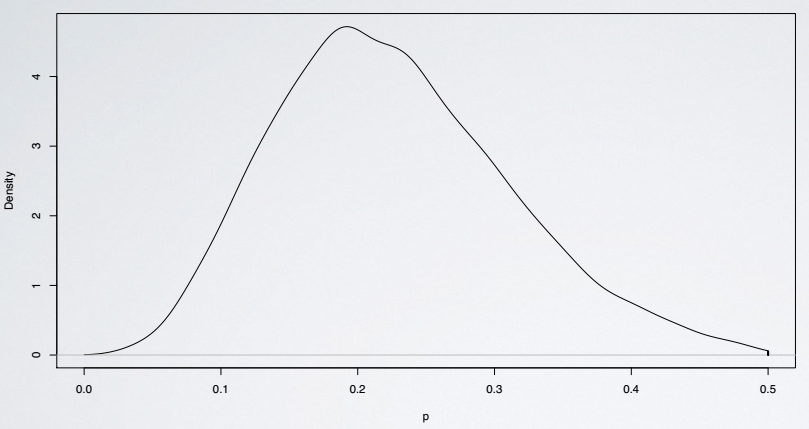
\includegraphics[width=11.24in]{JAGS_screenshot} 

}

\caption{Posterior with JAGS}\label{fig:JAGS-screenshot}
\end{figure}

That histogram is lightly smooth to generate the posterior density you
see. There is still a point mass of probability at 0.5, but now it has
less weight than before. Also, note how the data have changed the
posterior away from the prior. The analyst sees a lot of probability
under the curve near 0.2, but responds to the fact that no children were
born to RU-486 mothers.

This section is mostly a look-ahead to future material. We have seen
that a Bayesian might reasonably employ a non-conjugate prior in a
practical application. But then she will need to employ some kind of
numerical computation to approximate the posterior distribution.
Additionally, we have used a computational tool, JAGS, to approximate
the posterior for \(p\), and identified its three important elements,
the probability of the data given \(p\), that is the likelihood, and the
prior, and the call to the Gibbs sampler.

\subsection{Credible Intervals}\label{credible-intervals}

In this section, we introduce credible intervals, the Bayesian
alternative to confidence intervals. Let's start with the confidence
intervals, which are the frequentist way to express uncertainty about an
estimate of a population mean, a population proportion or some other
parameter.

A confidence interval has the form of an upper and lower bound.

\[L, U = \text{pe} \pm \text{se} \times \text{cv}\]

\begin{itemize}
\tightlist
\item
  L = lower, U = upper
\item
  pe = point estimate, se = standard error, cv = critical value
\end{itemize}

Most importantly, the interpretation of a 95\% confidence interval on
the mean is that \textbf{``95\% of similarly constructed intervals will
contain the true mean''}, not ``the probability that true mean lies
between \(L\) and \(U\) is 0.95''.

The reason for this frequentist wording is that a frequentist may not
express his uncertainty as a probability. The true mean is either within
the interval or not, so the probability is zero or one. The problem is
that the frequentist does not know which is the case.

On the other hand, Bayesians have no such qualms. It is fine for us to
say that \textbf{``the probability that the true mean is contained
within a given interval is 0.95''}. To distinguish our intervals from
confidence intervals, we call them \textbf{credible intervals}.

Recall the RU-486 example. When the analyst used the beta-binomial
family, she took the prior as \(p \sim \text{beta}(1,1)\), the uniform
distribution, where \(p\) is the probability of a child having a mother
who received RU-486.

After we observed four children born to mothers who received
conventional therapy, her posterior is \(p|x \sim \text{beta}(1,5)\). In
Figure \ref{fig:posterior}, the posterior probability density for
\(\text{beta}(1,5)\) puts a lot of probability near zero and very little
probability near one.

\begin{figure}
\centering
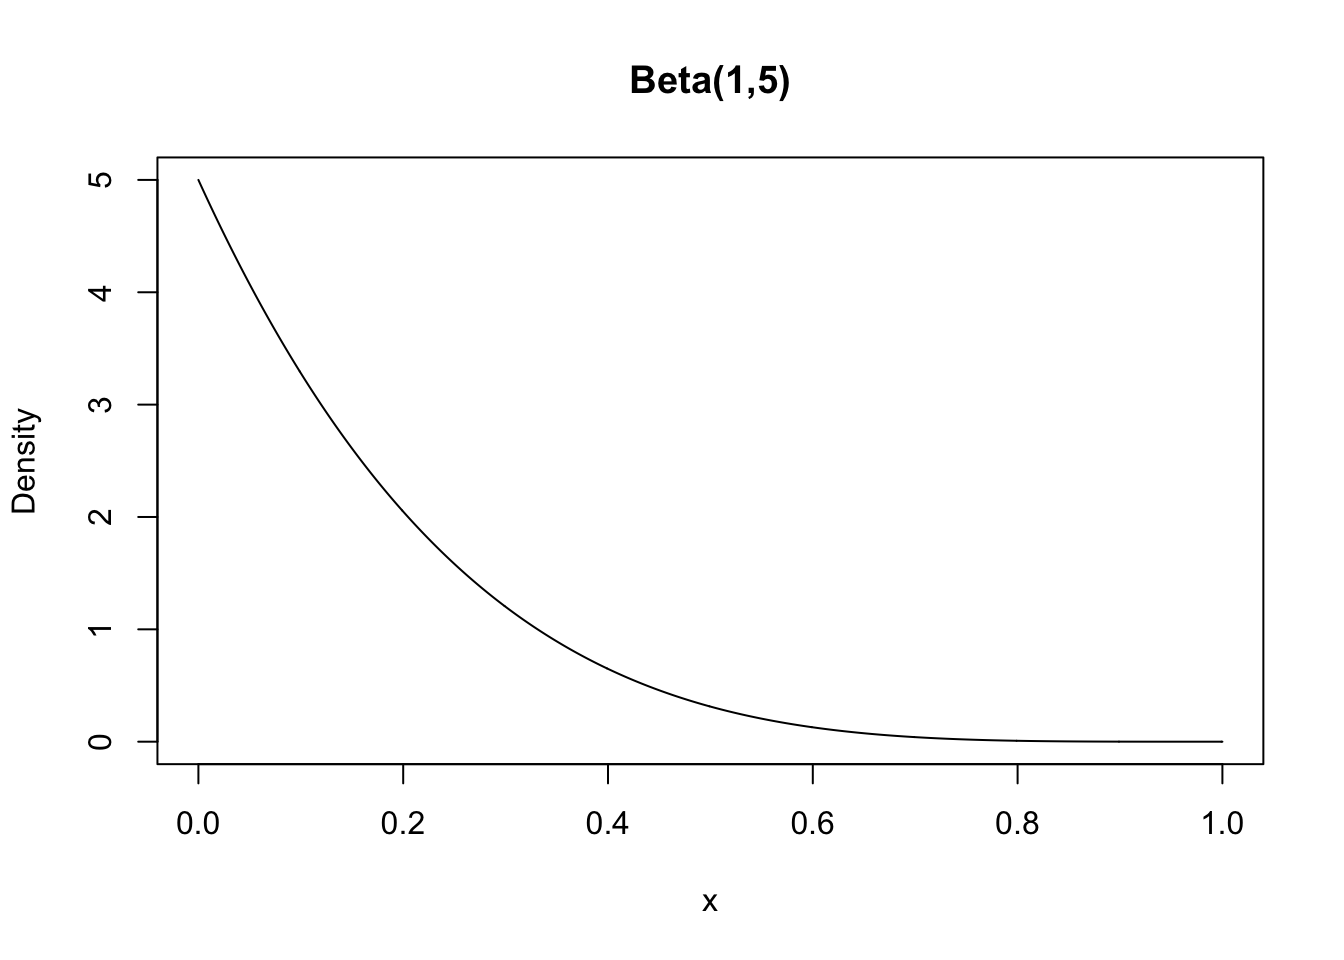
\includegraphics{02-inference-03-credible_files/figure-latex/posterior-1.pdf}
\caption{\label{fig:posterior}RU-486 Posterior}
\end{figure}

For the Bayesian, her 95\% credible interval is just any \(L\) and \(U\)
such that the posterior probability that \(L < p < U\) is \(0.95\). The
shortest such interval is obviously preferable.

To find this interval, the Bayesian looks at the area under the
\(\text{beta}(1,5)\) distribution, that lies to the left of a value x.

The density of the \(\text{beta}(1,5)\) is
\[f(p) = 5 (1-p)^4 \text{ for } 0 \leq p \leq 1,\]

and the area under the density between \(0\) and \(x\) is
\[F(x) = 1 - (1-x)^5 \text{ for } 0 \leq p \leq 1.\]

The Bayesian can use this to find \(L, U\) with area 0.95 under the
density curve between them, i.e. \(F(U) − F(L) = 0.95\). Note that the
Bayesian credible interval is asymmetric, unlike the symmetric
confidence intervals that frequentists often obtain. It turns out that
\(L = 0\) and \(U = 0.45\) is the shortest interval with probability
0.95 of containing \(p\).

What have we done? We have seen the difference in interpretations
between the frequentist confidence interval and the Bayesian credible
interval. Also, we have seen the general form of a credible interval.
Finally, we have done a practical example constructing a 95\% credible
interval for the RU-486 data set.

\subsection{Predictive Inference}\label{predictive-inference}

Predictive inference arises when the goal is not to find a posterior
distribution over some parameter, but rather to find a posterior
distribution over some random variable depends on the parameter.

Specifically, we want to make an inference on a random variable \(X\)
with probability densifity function \(f(x|\theta)\), where you have some
personal probability distribution \(\pi(\theta)\) for the \(\theta\).

To solve this, one needs to integrate:
\[P(X \leq x) = \int^{\infty}_{-\infty} P(X \leq x | \theta)\pi(\theta)d\theta\]

The equation gives us the weighted average of the probabilities for
\(X\), where the weights correspond to the personal probability on
\(\theta\). But we won't do an integral; instead, we will illustrate the
thinking with a trivial example.

\BeginKnitrBlock{example}
\protect\hypertarget{exm:unnamed-chunk-1}{}{\label{exm:unnamed-chunk-1}
}Suppose you have two coins. One coin has probability 0.7 of coming up
heads, and the other has probability 0.4 of coming up heads. You are
playing a gambling game with a friend, and you draw one of those two
coins at random from a bag.

Before you start the game, your prior belief is that the probability of
choosing the 0.7 coin is 0.5. This is reasonable, because both coins
were equally likely to be drawn. In this game, you win if the coin comes
up heads.

Suppose the game starts, you have tossed twice, and have obtained two
heads. Then what is your new belief about \(p\), the probability that
you are using the 0.7 coin?
\EndKnitrBlock{example}

This is just a simple application of the discrete form of Bayes' rule.

\begin{itemize}
\tightlist
\item
  Prior: \(p=0.5\)
\item
  Posterior:
  \[p^* = \frac{P(\text{2 heads}|0.7) \times 0.5}{P(\text{2 heads}|0.7) \times 0.5 + P(\text{2 heads}|0.4) \times 0.5} = 0.754.\]
\end{itemize}

However, this does not answer the important question -- What is the
predictive probability that the next toss will come up heads? This is of
interest because you are gambling on getting heads.

Fortunately, the predictive probablity of getting heads is not difficult
to calculate:

\begin{itemize}
\tightlist
\item
  \(p^* \text{ of 0.7 coin } = 0.754\)
\item
  \(p^* \text{ of 0.4 coin } = 1 − 0.754 = 0.246\)
\item
  \(P(\text{heads}) = P(\text{heads} | 0.7) \times 0.754 + P(\text{heads} | 0.4) \times 0.246 = 0.626\)
\end{itemize}

Therefore, the predictive probability that the next toss will come up
heads is 0.626.

Note that most realistic predictive inference problems are more
complicated and require one to use integrals. For example, one might
want to know the chance that a fifth child born in the RU-486 clinical
trial will have a mother who received RU-486. Or you might want to know
the probability that your stock broker's next recommendation will be
profitable.

We have learned three things in this section. First, often the real goal
is \textbf{a prediction about the value of a future random variable},
rather than making an estimate of a parameter. Second, these are deep
waters, and often one needs to integrate. Finally, in certain simple
cases where the parameter can only take discrete values, one can find a
solution without integration. In our example, the parameter could only
take two values to indicate which of the two coins was being used.

\chapter{Introduction to Losses and
Decision-making}\label{introduction-to-losses-and-decision-making}

In the previous chapter, we learned about continuous random variables.
That enabled us to study conjugate families, such as the beta binomial,
the poisson gamma, and the normal normal. We also considered the
difficulties of eliciting a personal prior, and of handling inference in
nonconjugate cases. Finally, we introduced the credible interval and
studied predictive inference.

In this new chapter, we will introduce loss functions and Bayesian
decision making, minimizing expected loss for hypothesis testing, and
define posterior probabilities of hypothesis and base factors. We will
then outline Bayesian testing for two proportions and two means, discuss
how findings from credible intervals compare to those from our
hypothesis test, and finally discuss when to reject, accept, or wait.

\section{Losses and Decision Making}\label{losses-and-decision-making}

To a Bayesian, the posterior distribution is the basis of any inference,
since it integrates both his/her prior opinions and knowledge and the
new information provided by the data. It also contains everything she
believes about the distribution of the unknown parameter of interest.

However, the posterior distribution on its own is not always sufficient.
Sometimes the inference we want to express is a \textbf{credible
interval}, because it indicates a range of likely values for the
parameter. That would be helpful if you wanted to say that you are
\textbf{95\% certain} the probability of an RU-486 pregnancy lies
between some number \(L\) and some number \(U\). And on other occasions,
one needs to make a single number guess about the value of the
parameter. For example, you might want to declare the average payoff for
an insurance claim or tell a patient how much longer he/she has to live.

Therefore, the Bayesian perspective leads directly to \textbf{decision
theory}. And in decision theory, one seeks to minimize one's expected
loss.

\subsection{Loss Functions}\label{loss-functions}

Quantifying the loss can be tricky, and Table \ref{tab:loss-functions}
summarizes three different examples with three different loss functions.

If you're declaring the average payoff for an insurance claim, and if
you are \textbf{linear} in how you value money, that is, twice as much
money is exactly twice as good, then one can prove that the optimal
one-number estimate is the \textbf{median} of the posterior
distribution. But in different situations, other measures of loss may
apply.

If you are advising a patient on his/her life expectancy, it is easy to
imagine that large errors are far more problematic than small ones. And
perhaps the loss increases as the \textbf{square} of how far off your
single number estimate is from the truth. For example, if she's told
that her average life expectancy is two years, and it is actually ten,
then her estate planning will be catastrophically bad, and she will die
in poverty. In the case when the loss is proportional to the
\textbf{quadratic} error, one can show that the optimal one-number
estimate is the \textbf{mean} of the posterior distribution.

Finally, in some cases, the penalty is 0 if you are exactly correct, but
constant if you're at all wrong. This is the case with the old saying
that close only counts with horseshoes and hand grenades; i.e., coming
close but not succeeding is not good enough. And it would apply if you
want a prize for correctly guessing the number of jelly beans in a jar.
Here, of course, instead of minimizing expected losses, we want to
\textbf{maximize the expected gain}. If a Bayesian is in such a
situation, then his/her best one-number estimate is the \textbf{mode} of
his/her posterior distribution, which is the most likely value.

There is a large literature on decision theory, and it is directly
linked to risk analysis, which arises in many fields. Although it is
possible for frequentists to employ a certain kind of decision theory,
it is much more natural for Bayesians.

\begin{table}

\caption{\label{tab:loss-functions}Loss Functions}
\centering
\begin{tabular}[t]{cc}
\toprule
Loss & Best Estimate\\
\midrule
Linear & Median\\
Quadratic & Mean\\
0/1 & Mode\\
\bottomrule
\end{tabular}
\end{table}

When making point estimates of unknown parameters, we should make the
choices that minimize the loss. Nevertheless, the best estimate depends
on the kind of loss function we are using, and we will discuss in more
depth how these best estimates are determined in the next section.

\subsection{Working with Loss
Functions}\label{working-with-loss-functions}

Now we illustrate why certain estimates minimize certain loss functions.

\BeginKnitrBlock{example}
\protect\hypertarget{exm:car}{}{\label{exm:car} }You work at a car
dealership. Your boss wants to know how many cars the dealership will
sell per month. An analyst who has worked with past data from your
company provided you a distribution that shows the probability of number
of cars the dealership will sell per month. In Bayesian lingo, this is
called the posterior distribution. A dot plot of that posterior is shown
in Figure \ref{fig:posterior-decision}. The mean, median and the mode of
the distribution are also marked on the plot. Your boss doesn't know any
Bayesian statistics though, so he/she wants you to report \textbf{a
single number} for the number of cars the dealership will sell per
month.
\EndKnitrBlock{example}

\begin{figure}

{\centering 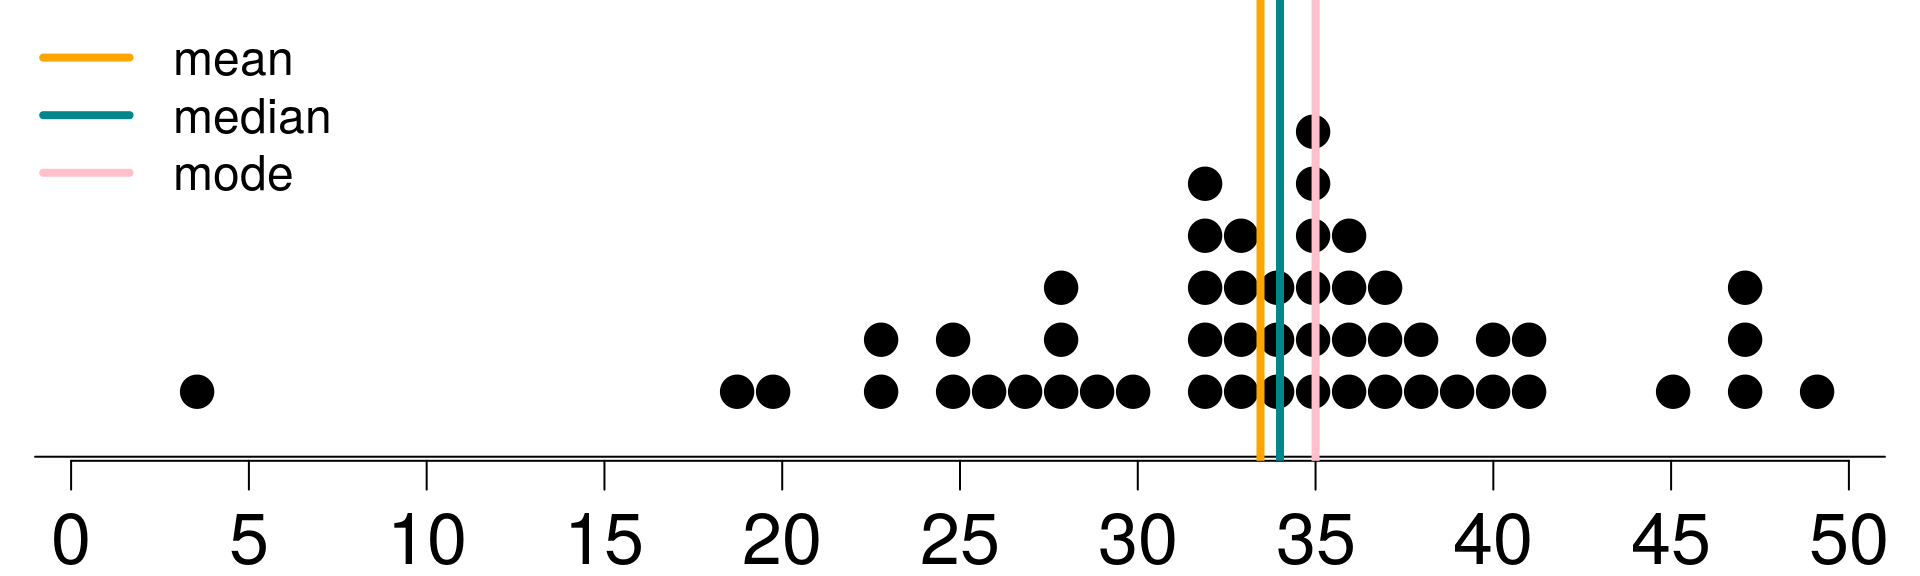
\includegraphics{03-decision-01-decisions_files/figure-latex/posterior-decision-1} 

}

\caption{Posterior}\label{fig:posterior-decision}
\end{figure}

Suppose your single guess is 30, and we call this \(g\) in the following
calculations. If your loss function is \(L_0\) (i.e., a 0/1 loss), then
you lose a point for each value in your posterior that differs from your
guess and do not lose any points for values that exactly equal your
guess. The total loss is the sum of the losses from each value in the
posterior.

In mathematical terms, we define \(L_0\) (0/1 loss) as

\[L_{0,i}(0,g) = \left\{ \begin{array}{cc}
0 & \text{if } g=x_i \\ 1 & \text{otherwise}
\end{array}\right.\]

The total loss is \(L_0 = \sum_i L_{0,i}(0,g)\).

Let's calculate what the total loss would be if your guess is 30. Table
\ref{tab:L0-table} summarizes the values in the posterior distribution
sorted in descending order.

The first value is 4, which is not equal to your guess of 30, so the
loss for that value is 1. The second value is 19, also not equal to your
guess of 30, and the loss for that value is also 1. The third value is
20, also not equal to your guess of 30, and the loss for this value is
also 1.

There is only one 30 in your posterior, and the loss for this value is 0
-- since it's equal to your guess (good news!). The remaining values in
the posterior are all different than 30 hence, the loss for them are all
ones as well.

To find the total loss, we simply sum over these individual losses in
the posterior distribution with 51 observations where only one of them
equals our guess and the remainder are different. Hence, the total loss
is 50.

Figure \ref{fig:L0-mode} is a visualization of the posterior
distribution, along with the 0-1 loss calculated for a series of
possible guesses within the range of the posterior distribution. To
create this visualization of the loss function, we went through the
process we described earlier for a guess of 30 for all guesses
considered, and we recorded the total loss. We can see that the loss
function has the lowest value when \(g\), our guess, is equal to
\textbf{the most frequent observation} in the posterior. Hence, \(L_0\)
is minimized at the \textbf{mode} of the posterior, which means that if
we use the 0/1 loss, the best point estimate is the mode of the
posterior.

\begin{table}

\caption{\label{tab:L0-table}L0: 0/1 loss for g = 30}
\centering
\begin{tabular}[t]{ccc}
\toprule
i & x\_i & L0: 0/1\\
\midrule
1 & 4 & 1\\
2 & 19 & 1\\
3 & 20 & 1\\
 & ... & ...\\
14 & 30 & 0\\
\addlinespace
 & ... & ...\\
50 & 47 & 1\\
51 & 49 & 1\\
 & Total & 50\\
\bottomrule
\end{tabular}
\end{table}

\begin{figure}

{\centering 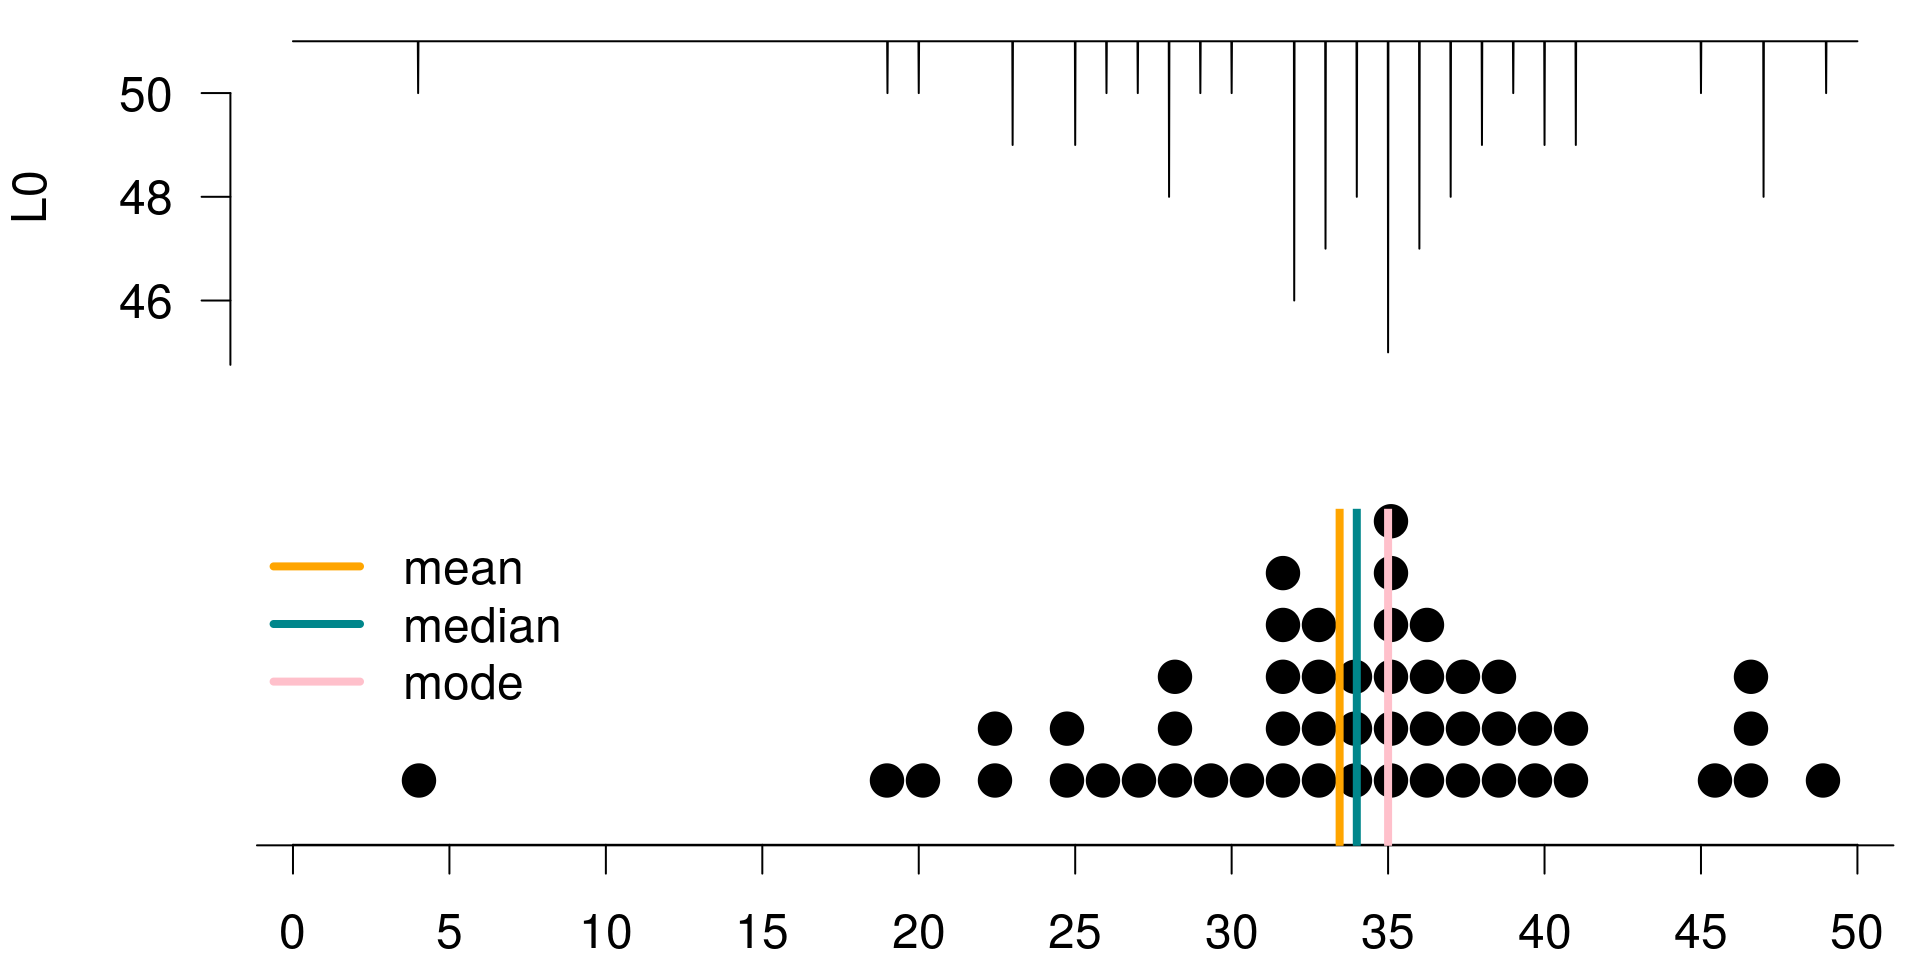
\includegraphics{03-decision-01-decisions_files/figure-latex/L0-mode-1} 

}

\caption{L0 is minimized at the mode of the posterior}\label{fig:L0-mode}
\end{figure}

Let's consider another loss function. If your loss function is \(L_1\)
(i.e., linear loss), then the total loss for a guess is the sum of the
\textbf{absolute values} of the difference between that guess and each
value in the posterior. Note that the absolute value function is
required, because overestimates and underestimates do not cancel out.

In mathematical terms, \(L_1\) (linear loss) is calculated as
\(L_1(g) = \sum_i |x_i - g|\).

We can once again calculate the total loss under \(L_1\) if your guess
is 30. Table \ref{tab:L1-table} summarizes the values in the posterior
distribution sorted in descending order.

The first value is 4, and the absolute value of the difference between 4
and 30 is 26. The second value is 19, and the absolute value of the
difference between 19 and 30 is 11. The third value is 20 and the
absolute value of the difference between 20 and 30 is 10.

There is only one 30 in your posterior, and the loss for this value is 0
since it is equal to your guess. The remaining value in the posterior
are all different than 30 hence their losses are different than 0.

To find the total loss, we again simply sum over these individual
losses, and the total is to 346.

Again, Figure \ref{fig:L1-median} is a visualization of the posterior
distribution, along with a linear loss function calculated for a series
of possible guesses within the range of the posterior distribution. To
create this visualization of the loss function, we went through the same
process we described earlier for all of the guesses considered. This
time, the function has the lowest value when \(g\) is equal to the
\textbf{median} of the posterior. Hence, \(L_1\) is minimized at the
\textbf{median} of the posterior one other loss function.

\begin{table}

\caption{\label{tab:L1-table}L1: linear loss for g = 30}
\centering
\begin{tabular}[t]{ccc}
\toprule
i & x\_i & L1: |x\_i-30|\\
\midrule
1 & 4 & 1\\
2 & 19 & 1\\
3 & 20 & 1\\
 & ... & ...\\
14 & 30 & 0\\
\addlinespace
 & ... & ...\\
50 & 47 & 1\\
51 & 49 & 1\\
 & Total & 346\\
\bottomrule
\end{tabular}
\end{table}

\begin{figure}

{\centering 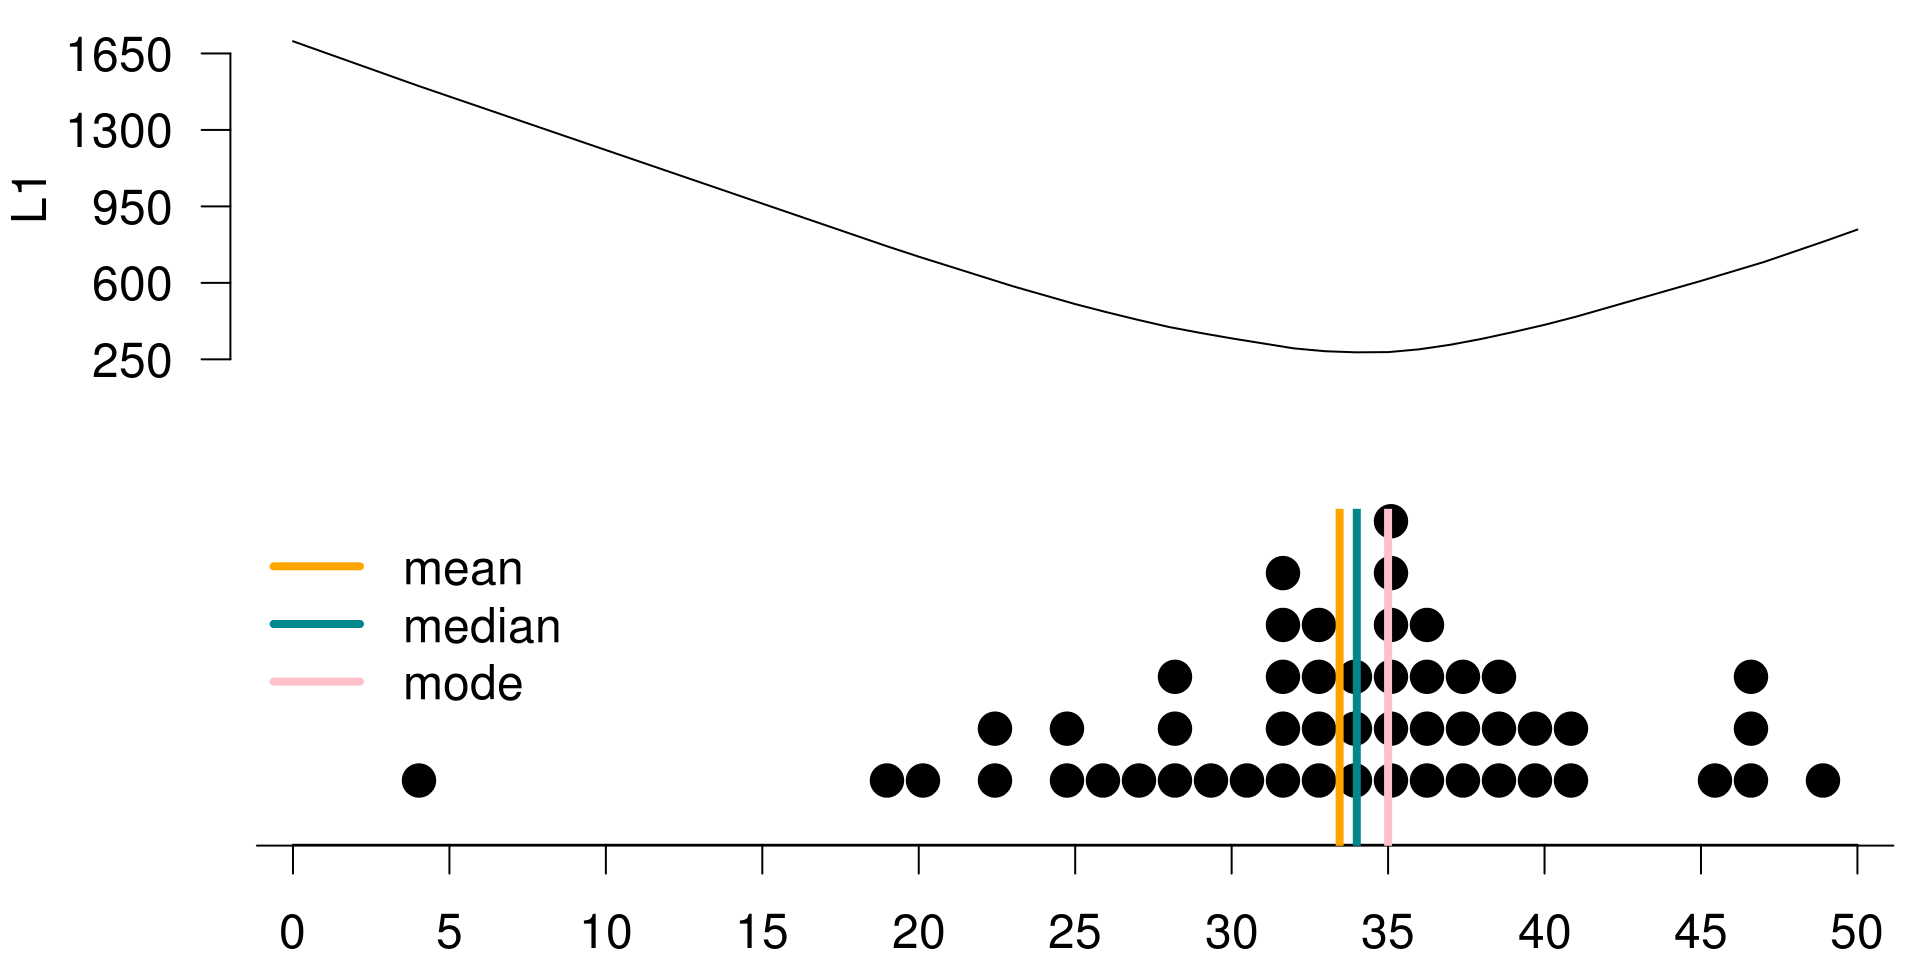
\includegraphics{03-decision-01-decisions_files/figure-latex/L1-median-1} 

}

\caption{L1 is minimized at the median of the posterior}\label{fig:L1-median}
\end{figure}

If your loss function is \(L_2\) (i.e.~a squared loss), then the total
loss for a guess is the sum of the squared differences between that
guess and each value in the posterior.

We can once again calculate the total loss under \(L_2\) if your guess
is 30. Table \ref{tab:L2-table} summarizes the posterior distribution
again, sorted in ascending order.

The first value is 4, and the squared difference between 4 and 30 is
676. The second value is 19, and the square of the difference between 19
and 30 is 121. The third value is 20, and the square difference between
20 and 30 is 100.

There is only one 30 in your posterior, and the loss for this value is 0
since it is equal to your guess. The remaining values in the posterior
are again all different than 30, hence their losses are all different
than 0.

To find the total loss, we simply sum over these individual losses again
and the total loss comes out to 3,732. We have the visualization of the
posterior distribution. Again, this time along with the squared loss
function calculated for a possible serious of possible guesses within
the range of the posterior distribution.

Creating the visualization in Figure \ref{fig:L2-mean} had the same
steps. Go through the same process described earlier for a guess of 30,
for all guesses considered, and record the total loss. This time, the
function has the lowest value when \(g\) is equal to the \textbf{mean}
of the posterior. Hence, \(L_2\) is minimized at the \textbf{mean} of
the posterior distribution.

\begin{table}

\caption{\label{tab:L2-table}L2: squared loss for g = 30}
\centering
\begin{tabular}[t]{ccc}
\toprule
i & x\_i & L2: (x\_i-30)\textasciicircum{}2\\
\midrule
1 & 4 & 1\\
2 & 19 & 1\\
3 & 20 & 1\\
 & ... & ...\\
14 & 30 & 0\\
\addlinespace
 & ... & ...\\
50 & 47 & 1\\
51 & 49 & 1\\
 & Total & 3732\\
\bottomrule
\end{tabular}
\end{table}

\begin{figure}

{\centering 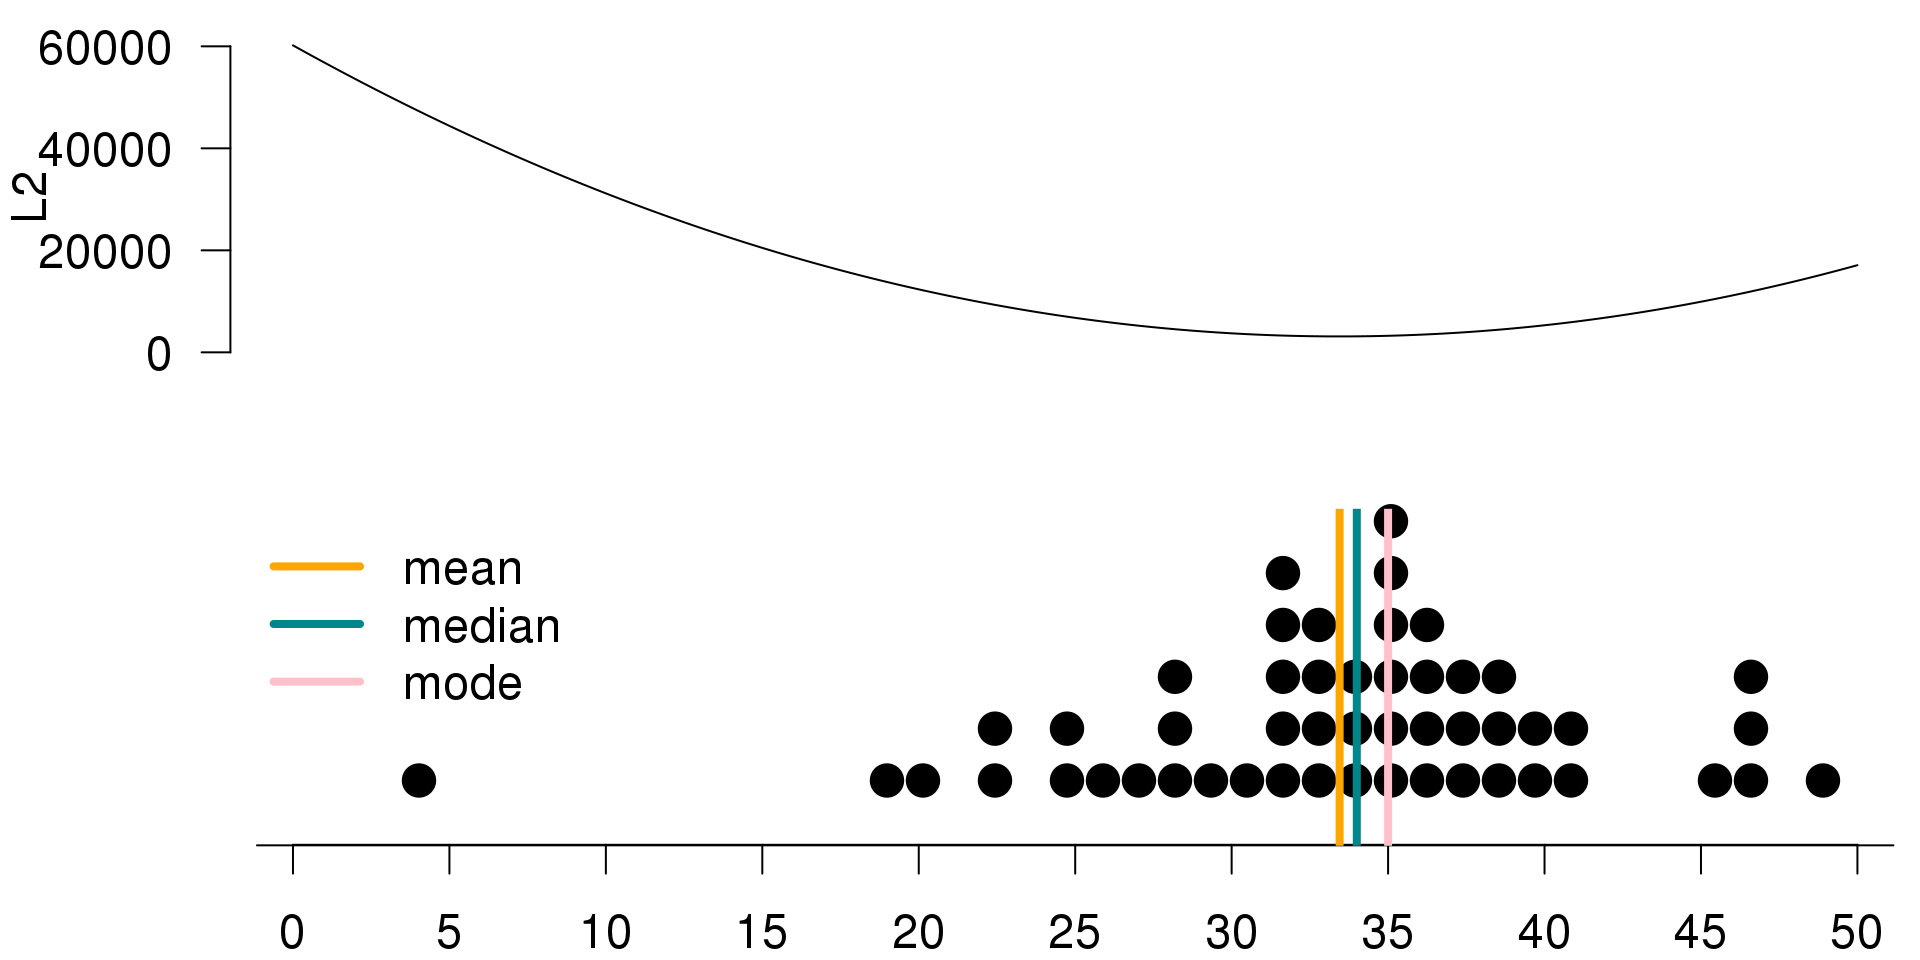
\includegraphics{03-decision-01-decisions_files/figure-latex/L2-mean-1} 

}

\caption{L2 is minimized at the mean of the posterior}\label{fig:L2-mean}
\end{figure}

To sum up, the point estimate to report to your boss about the number of
cars the dealership will sell per month \textbf{depends on your loss
function}. In any case, you will choose to report the estimate that
minimizes the loss.

\begin{itemize}
\tightlist
\item
  \(L_0\) is minimized at the \textbf{mode} of the posterior
  distribution.
\item
  \(L_1\) is minimized at the \textbf{median} of the posterior
  distribution.
\item
  \(L_2\) is minimized at the \textbf{mean} of the posterior
  distribution.
\end{itemize}

\subsection{Minimizing Expected Loss for Hypothesis
Testing}\label{minimizing-expected-loss-for-hypothesis-testing}

In Bayesian statistics, the inference about a parameter is made based on
the posterior distribution, and let's include this in the hypothesis
test setting.

Suppose we have two competing hypothesis, \(H_1\) and \(H_2\). Then we
get

\begin{itemize}
\tightlist
\item
  \(P(H_1 \text{ is true } | \text{ data})\) = posterior probability of
  \(H_1\)
\item
  \(P(H_2 \text{ is true } | \text{ data})\) = posterior probability of
  \(H_2\)
\end{itemize}

One straightforward way of choosing between \(H_1\) and \(H_2\) would be
to \textbf{choose the one with the higher posterior probability}. In
other words, the potential decision criterion is to

\begin{itemize}
\tightlist
\item
  Reject \(H_1\) if
  \(P(H_1 \text{ is true } | \text{ data}) < P(H_1 \text{ is true } | \text{ data})\).
\end{itemize}

However, since hypothesis testing is a decision problem, we should also
consider a loss function. Let's revisit the HIV testing example in
Section \ref{sec:diagnostic-testing}, and suppose we want to test the
two competing hypotheses below:

\begin{itemize}
\tightlist
\item
  \(H_1\): Patient does not have HIV
\item
  \(H_2\): Patient has HIV
\end{itemize}

These are the only two possibilities, so they are mutually exclusive
hypotheses that cover the entire decision space.

We can define the loss function as \(L(d)\) -- the loss that occurs when
decision \(d\) is made. Then the Bayesian testing procedure minimizes
the posterior expected loss.

The possible decisions (actions) are:

\begin{itemize}
\tightlist
\item
  \(d_1\): Choose \(H_1\) - decide that the patient does not have HIV
\item
  \(d_2\): Choose \(H_2\) - decide that the patient has HIV
\end{itemize}

For each decision \(d\), we might be right, or we might be wrong. If the
decision is right, the loss \(L(d)\) associated with the decision \(d\)
is zero, i.e.~no loss. If the decision is wrong, the loss \(L(d)\)
associated with the decision \(d\) is some positive value \(w\).

For \(d=d_1\), we have

\begin{itemize}
\tightlist
\item
  \textbf{Right}: Decide patient does not have HIV, and indeed they do
  not. \(\Rightarrow L(d_1) = 0\)
\item
  \textbf{Wrong}: Decide patient does not have HIV, but they do.
  \(\Rightarrow L(d_1) = w_1\)
\end{itemize}

For \(d=d_2\), we also have

\begin{itemize}
\tightlist
\item
  \textbf{Right}: Decide patient has HIV, and indeed they do.
  \(\Rightarrow L(d_2) = 0\)
\item
  \textbf{Wrong}: Decide patient has HIV, but they don't
  \(\Rightarrow L(d2) = w_2\)
\end{itemize}

The consequences of making a wrong decision \(d_1\) or \(d_2\) are
different.

Wrong \(d_1\) is a \textbf{false negative}:

\begin{itemize}
\tightlist
\item
  We decide that patient does not have HIV when in reality they do.
\item
  Potential consequences: no treatment and premature death! (severe)
\end{itemize}

Wrong \(d_2\) is a \textbf{false positive}:

\begin{itemize}
\tightlist
\item
  We decide that the patient has HIV when in reality they do not.
\item
  Potential consequences: distress and unnecessary further
  investigation. (not ideal but less severe than the consequences of a
  false negative decision)
\end{itemize}

Let's put these definitions in the context of the HIV testing example
with ELISA.

\textbf{Hypotheses}

\begin{itemize}
\tightlist
\item
  \(H_1\): Patient does not have HIV
\item
  \(H_2\): Patient has HIV
\end{itemize}

\textbf{Decision}

\begin{itemize}
\tightlist
\item
  \(d_1\): Choose \(H_1\) - decide that the patient does not have HIV
\item
  \(d_2\): Choose \(H_2\) - decide that the patient has HIV
\end{itemize}

\textbf{Losses}

\begin{itemize}
\item
  \(L(d_1) = \left\{ \begin{array}{cc} 0 & \text{if $d_1$ is right}\\ w_1=1000 & \text{if $d_1$ is wrong} \end{array}\right.\)
\item
  \(L(d_2) = \left\{ \begin{array}{cc} 0 & \text{if $d_2$ is right}\\ w_2=10 & \text{if $d_2$ is wrong} \end{array}\right.\)
\end{itemize}

The values of \(w_1\) and \(w_2\) are arbitrarily chosen. But the
important thing is that \(w_1\), the loss associated with a false
negative determination, is much higher than \(w_2\), the loss associated
with a false positive determination.

\textbf{Posteriors}

The plus sign means that our patient had tested positive on the ELISA.

\begin{itemize}
\tightlist
\item
  \(P(H_1|+) \approx 0.88\) - the posterior probability of the patient
  \textbf{not} having HIV given positive ELISA result
\item
  \(P(H_2|+) \approx 0.12\) - the posterior probability of the patient
  having HIV given positive ELISA result, as the complement value of
  \(P(H_1|+)\)
\end{itemize}

\textbf{Expected losses}

\begin{itemize}
\tightlist
\item
  \(E[L(d_1)] = 0.88 \times 0 + 0.12 \times 1000 = 120\)
\item
  \(E[L(d_2)] = 0.88 \times 10 + 0.12 \times 0 = 8.8\)
\end{itemize}

Since the expected loss for \(d_2\) is lower, we should make this
decision -- the patient has HIV.

Note that our decision is highly influenced by the losses we assigned to
\(d_1\) and \(d_2\).

If the losses were symmetric, say \(w_1 = w_2 = 10\), then the expected
loss for \(d_1\) becomes

\[E[L(d_1)] = 0.88 \times 0 + 0.12 \times 10 = 1.2,\]

while the expected loss for \(d_2\) would not change. Therefore, we
would choose \(d_1\) instead; that is, we would decide that the patient
does not have HIV.

To recap, Bayesian methodologies allow for the integration of losses
into the decision making framework easily. And in Bayesian testing, we
minimize the posterior expected loss.

\subsection{Posterior Probabilities of Hypotheses and Bayes
Factors}\label{posterior-probabilities-of-hypotheses-and-bayes-factors}

In this section, we will continue with the HIV testing example to
introduce the concept of Bayes factors. Earlier, we introduced the
concept of priors and posteriors. The \textbf{prior odds} is defined as
\textbf{the ratio of the prior probabilities of hypotheses}.

Therefore, if there are two competing hypotheses being considered, then
the prior odds of \(H_1\) to \(H_2\) can be defined as \(O[H_1:H_2]\),
which is equal to \(P(H_1)\) over probability of \(P(H_2)\). In
mathematical terms,

\[O[H_1:H_2] = \frac{P(H_1)}{P(H_2)}\]

Similarly, the \textbf{posterior odds} is \textbf{the ratio of the two
posterior probabilities of hypotheses}, written as

\[PO[H_1:H_2] = \frac{P(H_1|\text{data})}{P(H_2|\text{data})}\]

Using Bayes' rule, we can rewrite the posterior probabilities as below:

\[\begin{aligned}
PO[H_1:H_2] &= \frac{P(H_1|\text{data})}{P(H_2|\text{data})} \\
&= \frac{(P(\text{data}|H_1) \times P(H_1)) / P(\text{data}))}{(P(\text{data}|H_2) \times P(H_2)) / P(\text{data}))} \\
&= \frac{(P(\text{data}|H_1) \times P(H_1))}{(P(\text{data}|H_2) \times P(H_2))} \\
&= \boxed{\frac{P(\text{data}|H_1)}{P(\text{data}|H_2)}} \times \boxed{\frac{P(H_1)}{P(H_2)}} \\
&= \textbf{Bayes factor} \times \textbf{prior odds}
\end{aligned}\]

In mathematical notation, we have

\[PO[H_1:H_2] = BF[H_1:H_2] \times O[H_1:H_2]\]

In other words, the posterior odds is the product of the Bayes factor
and the prior odds for these two hypotheses.

The Bayes factor quantifies the evidence of data arising from \(H_1\)
versus \(H_2\).

In a discrete case, the Bayes factor is simply the ratio of the
likelihoods of the observed data under the two hypotheses, written as

\[BF[H_1:H_2] = \frac{P(\text{data}|H_1)}{P(\text{data}|H_2)}.\]

On the other hand, in a continuous case, the Bayes factor is the ratio
of the marginal likelihoods, written as

\[BF[H_1:H_2] = \frac{\int P(\text{data}|\theta,H_1)d\theta}{\int P(\text{data}|\theta,H_2)d\theta}.\]

Note that \(\theta\) is the set formed by all possible values of the
model parameters.

In this section, we will stick with the simpler discrete case. And in
upcoming sections, we will revisit calculating Bayes factors for more
complicated models.

Let's return to the HIV testing example from earlier, where our patient
had tested positive in the ELISA.

\textbf{Hypotheses}

\begin{itemize}
\tightlist
\item
  \(H_1\): Patient does not have HIV
\item
  \(H_2\): Patient has HIV
\end{itemize}

\textbf{Priors}

The prior probabilities we place on these hypothesis came from the
prevalence of HIV at the time in the general population. We were told
that the prevalence of HIV in the population was 1.48 out of 1000, hence
the prior probability assigned to \(H_2\) is 0.00148. And the prior
assigned to \(H_1\) is simply the complement of this.

\begin{itemize}
\tightlist
\item
  \(P(H_1) = 0.99852\) and \(P(H_2) = 0.00148\)
\end{itemize}

The prior odds are

\begin{itemize}
\tightlist
\item
  \(O[H_1:H_2] = \dfrac{P(H_1)}{P(H_2)} = \dfrac{0.99852}{0.00148} = 674.6757\)
\end{itemize}

\textbf{Posteriors}

Given a positive ELISA result, the posterior probabilities of these
hypotheses can also be calculated, and these are approximately 0.88 and
0.12. We will hold on to more decimal places in our calculations to
avoid rounding errors later.

\begin{itemize}
\tightlist
\item
  \(P(H_1|+) = 0.8788551\) and \(P(H_2|+) = 0.1211449\)
\end{itemize}

The posterior odds are

\begin{itemize}
\tightlist
\item
  \(PO[H_1:H_2] = \dfrac{P(H_1|+)}{P(H_2|+)} = \dfrac{0.8788551}{0.1211449} = 7.254578\)
\end{itemize}

\textbf{Bayes Factor}

Finally, we can calculate the Bayes factor as the ratio of the posterior
odds to prior odds, which comes out to approximately 0.0108. Note that
in this simple discrete case the Bayes factor, it simplifies to the
ratio of the likelihoods of the observed data under the two hypotheses.

\[\begin{aligned}
BF[H_1:H_2] &= \frac{PO[H_1:H_2]}{O[H_1:H_2]} = \frac{7.25457}{674.6757} \approx 0.0108 \\
&= \frac{P(+|H_1)}{P(+|H_2)} = \frac{0.01}{0.93} \approx 0.0108
\end{aligned}\]

Alternatively, remember that the true positive rate of the test was 0.93
and the false positive rate was 0.01. Using these two values, the Bayes
factor also comes out to approximately 0.0108.

So now that we calculated the Bayes factor, the next natural question
is, what does this number mean? A commonly used scale for interpreting
Bayes factors is proposed by \citet{jeffreys1961theory}, as in Table
\ref{tab:jeffreys1961}. If the Bayes factor is between 1 and 3, the
evidence against \(H_2\) is not worth a bare mention. If it is 3 to 20,
the evidence is positive. If it is 20 to 150, the evidence is strong. If
it is greater than 150, the evidence is very strong.

\begin{table}

\caption{\label{tab:jeffreys1961}Interpreting the Bayes factor}
\centering
\begin{tabular}[t]{cc}
\toprule
BF[H\_1:H\_2] & Evidence against H\_2\\
\midrule
1 to 3 & Not worth a bare mention\\
3 to 20 & Positive\\
20 to 150 & Strong\\
> 150 & Very strong\\
\bottomrule
\end{tabular}
\end{table}

It might have caught your attention that the Bayes factor we calculated
does not even appear on the scale. To obtain a Bayes factor value on the
scale, we will need to change the order of our hypotheses and calculate
\(BF[H_2:H_1]\), i.e.~the Bayes factor for \(H_2\) to \(H_1\). Then we
look for evidence against \(H_1\) instead.

We can calculate \(BF[H_2:H_1]\) as a reciprocal of \(BF[H_1:H_2]\) as
below:

\[BF[H_2:H_1] = \frac{1}{BF[H_1:H_2]} = \frac{1}{0.0108} = 92.59259\]

For our data, this comes out to approximately 93. Hence the evidence
against \(H_1\) (the patient does not have HIV) is strong. Therefore,
even though the posterior for having HIV given a positive result, i.e.
\(P(H_2|+)\), was low, we would still decide that the patient has HIV,
according to the scale based on a positive ELISA result.

An intuitive way of thinking about this is to consider not only the
posteriors, but also the priors assigned to these hypotheses. Bayes
factor is the ratio of the posterior odds to prior odds. While 12\% is a
low posterior probability for having HIV given a positive ELISA result,
this value is still much higher than the overall prevalence of HIV in
the population (in other words, the prior probability for that
hypothesis).

Another commonly used scale for interpreting Bayes factors is proposed
by \citet{kass1995bayes}, and it deals with the natural logarithm of the
calculated Bayes factor. The values can be interpreted in Table
\ref{tab:kass1995}.

\begin{table}

\caption{\label{tab:kass1995}Interpreting the Bayes factor}
\centering
\begin{tabular}[t]{cc}
\toprule
2*log(BF[H\_2:H\_1]) & Evidence against H\_1\\
\midrule
0 to 2 & Not worth a bare mention\\
2 to 6 & Positive\\
6 to 10 & Strong\\
> 10 & Very strong\\
\bottomrule
\end{tabular}
\end{table}

Reporting of the log scale can be helpful for numerical accuracy reasons
when the likelihoods are very small. Taking two times the natural
logarithm of the Bayes factor we calculated earlier, we would end up
with the same decision that the evidence against \(H_1\) is strong.

\[2 \times \log(92.59259) = 9.056418\]

To recap, we defined prior odds, posterior odds, and the Bayes factor.
We learned about scales by which we can interpret these values for model
selection. We also re-emphasize that in Bayesian testing, the order in
which we evaluate the models of hypotheses does \textbf{not} matter. The
Bayes factor of \(H_2\) versus \(H_1\), \(BF[H_2:H_1]\), is simply the
reciprocal of the Bayes factor for \(H_1\) versus \(H_2\), that is,
\(BF[H_1:H_2]\).

\section{Inference and Decision-Making with Multiple
Parameters}\label{inference-and-decision-making-with-multiple-parameters}

This section is focused on the extending the Normal-Normal conjugate
family introduced in \ref{sec:normal-normal} to the problem of inference
in a Normal population with an unknown mean and variance. We will
introduce the Normal-Gamma conjugate family for inference about the
unknown mean and variance and will present Monte Carlo simulation for
inference about functions of the parameters as well as sampling from
predictive distributions, which can assist with prior elucidation. For
situations when limited prior information is available, we discuss a
limiting case of the Normal-Gamma conjugate family, leading to priors
that can be used for a reference analysis. Finally, we will show how to
create a more flexible and robust prior distribution by using mixtures
of the Normal-Gamma conjugate prior. For inference in this case we will
introduce Markov Chain Monte Carlo, a powerful simulation method for
Bayesian inference.

It is assumed that the readers have mastered the concepts of
one-parameter Normal-Normal conjugate priors. Calculus is not required
for this section; however, for those who are comfortable with calculus
and would like to go deeper, we shall present starred sections with more
details on the derivations.

\subsection{The Normal-Gamma Conjugate Family}\label{sec:normal-gamma}

In \ref{sec:normal-normal} we described the normal-normal conjugate
family for inference about an unknown mean \(\mu\) with a known standard
deviation \(\sigma\) when the data were assumed to be a random sample
from a normal population. In this section we will introduce the
normal-gamma conjugate family for the common situation when \(\sigma\)
is unknown. As both \(\mu\) and \(\sigma^2\) unknown, we will need to
specify a \textbf{joint} prior distribution to describe our prior
uncertainty about them.

\textbf{Sampling Model}

Recall that a conjugate pair is a sampling model for the data and prior
distribution for the unknown parameters such that the posterior
distribution is in the same family of distributions as the prior
distribution. We will assume that the data are a random sample of size
\(n\) from a normal population with mean \(\mu\) and variance
\(\sigma^2\); the following is a mathematical shorthand to represent
this distribution assumption

\[\begin{aligned}
Y_1, \ldots Y_n  \iid
\textsf{N}(\mu, \sigma^2) 
\end{aligned}\] where the `iid' above the distributed as symbol
`\(\sim\)' indicates that each of the observations are
\textbf{i}ndependent of the others (given \(\mu\) and \(\sigma^2\)) and
are \textbf{i}dentically \textbf{d}istributed.

\textbf{Conjugate prior} Back in \ref{sec:normal-normal}, we found that
with normal data, the conjugate prior for \(\mu\) when the standard
deviation \(\sigma\) was known was a normal distribution. We will build
on this to specify a conditional prior distribution for \(\mu\) as

\begin{equation}
\mu \mid \sigma^2   \sim  \textsf{N}(m_0, \sigma^2/n_0)
\label{eq:04-conjugate-normal}
\end{equation}

with hyper-parameters \(m_0\), the prior mean for \(\mu\), and
\(\sigma^2/n_0\) the prior variance. While previously the variance was a
known constant \(\tau^2\), replacing \(\tau^2\) with a multiple of
\(\sigma^2\) is needed for representing the joint conjugate prior for
the mean and variance. Because \(\sigma\) has the same units as the
data, the hyper-parameter \(n_0\) is unitless, but is used to express
our prior precision about \(\mu\) with larger values of \(n_0\)
indicating more precision and smaller values less precision. We will see
later how the hyper-parameter \(n_0\) may be interpreted as a prior
sample size.

As \(\sigma^2\) is unknown, a Bayesian would use a prior distribution to
describe the uncertainty about the variance before seeing data. Since
the variance is non-negative, continuous, and with no upper limit, a
gamma distribution is a candidate prior for the variance, based on the
distributions that we have seen so far. However, that choice does not
lead to a posterior distribution in the same family or that is
recognizable as any common distribution. It turns out that the the
inverse of the variance, which is known as the precision, has a
conjugate gamma prior distribution. Letting \(\phi = 1/\sigma^2\) denote
the precision or inverse variance, the conjugate prior for \(\phi\),

\begin{equation}
\phi \sim \textsf{Gamma}\left(\frac{v_0}{2}, \frac{v_0 s^2_0}{2} \right)
\label{eq:04-conjugate-gamma}
\end{equation}

is a gamma distribution with hyper-parameters \(v_0\), prior degrees of
freedom, and \(s^2_0\) a prior variance or guess for \(\sigma^2\).
Equivalently we may say that the inverse of the variance has a
\[1/\sigma^2 \sim \textsf{Gamma}(v_0/2, s^2_0 v_0/2)\]

gamma distribution to avoid using a new symbol. Together the Normal
conditional distribution for \(\mu\) given \(\sigma^2\) in
\eqref{eq:04-conjugate-normal} and the marginal Gamma distribution for
\(\phi\) in \eqref{eq:04-conjugate-gamma} lead to a joint distribution for
the pair \((\mu, \phi)\) that we will call the Normal-Gamma family of
distributions:

\begin{equation}(\mu, \phi) \sim \textsf{NormalGamma}(m_0, n_0, s^2_0, v_0)
\label{eq:04-conjugate-normal-gamma}
\end{equation}

with the four hyper-parameters \(m_0\), \(n_0\), \(s^2_0\), and \(v_0\).

\textbf{Posterior Distribution}

As a conjugate family, the posterior distribution of the pair of
parameters (\(\mu, \phi\)) is in the same family as the prior
distribution when the sample data arise from a normal distribution, that
is the posterior is also Normal-Gamma

\begin{equation}
(\mu, \phi) \mid \text{data} \sim \textsf{NormalGamma}(m_n, n_n, s^2_n, v_n)
\end{equation}

where the subscript \(n\) on the hyper-parameters indicates the updated
values after seeing the \(n\) observations. One attraction to conjugate
families is there are relatively simple updating rules for obtaining the
new hyper-parameters:

\begin{eqnarray*}
m_n & = & \frac{n \bar{Y} + n_0 m_0} {n + n_0}  \\
& \\
n_n & = & n_0 + n  \\
v_n & = & v_0 + n  \\
s^2_n & =  & \frac{1}{v_n}\left[s^2_0 v_0 + s^2 (n-1) + \frac{n_0 n}{n_n} (\bar{Y} - m_0)^2 \right]. 
\end{eqnarray*}

The updated hyper-parameter \(m_n\) in the posterior distribution of
\(\mu\) is the posterior mean, which is a weighted average of the sample
mean \(\bar{Y}\) and prior mean \(m_0\) with weights \(n/(n + n_0\) and
\(n_0/(n + n_0)\) respectively and does not depend on \(\sigma^2\). The
posterior sample size \(n_n\) is the sum of the prior sample size
\(n_n\) and the sample size \(n\), representing the combined precision
of the estimate for \(\mu\). The posterior degrees of freedom \(v_n\)
are also increased by adding the sample size \(n\) to the prior degrees
of freedom \(v_0\). Finally, the posterior variance hyper-parameter
\(s^2_n\) combines three sources of information about \(\sigma\) in
terms of sums of squared deviations. \textbf{FILL IN MORE DETAILS} The
first term in the square brackets is the sample variance times the
sample degrees of freedom which is the sample sum of squares. The second
term represents the prior sum of squares, while the third term is based
on the squared difference of the sample mean and prior mean. We then
divide by the posterior degrees of freedom to get the new
hyper-parameter.

The joint Normal-Gamma distribution for the pair \(\mu\) and \(\phi\),
\[(\mu, \phi) \mid \data \sim \NoGa(m_n, n_n, s^2_n, v_n)\] is
equivalent to a \textbf{hierarchical model} specified in two stages with
\(\mu\) given \(\sigma\) having a conditional normal distribution
\[\mu \mid \data, \sigma^2  \sim  \No(m_n, \sigma^2/n_n)\] and the
inverse variance marginally \[
1/\sigma^2 \mid \data   \sim   \Ga(v_n/2, s^2_n v_n/2) 
\] having a gamma distribution. We will see in the next section how this
representation is convenient for generating samples from the posterior
distribution.

\textbf{Marginal Distribution for \(\mu\)}

We are generally interested in inference about \(\mu\) unconditionally
as \(\sigma^2\) is unknown. This marginal inference requires the
unconditional or marginal distribution of \(\mu\) that `averages' over
the uncertainty in \(\sigma\). For continuous variables like \(\sigma\),
this averaging is performed by integration leading to the following
result:

\(\mu\) given the data is a \index{Student t distribution}
\[ \mu \mid \data \sim \St(v_n, m_n, s^2_n/n_n)  \] with density

\begin{equation}
p(\mu) =\frac{\Gamma\left(\frac{v_n + 1}{2} \right)}
{\sqrt{\pi v_n} \frac{s_n}{\sqrt{n_n}} \,\Gamma\left(\frac{v_n}{2} \right)}
\left(1 + \frac{1}{v_n}\frac{(\mu - m_n)^2} {s^2_n/n_n} \right)^{-\frac{v_n+1}{2}} 
\label{eq:Student-t-density}
\end{equation}

with the degrees of freedom \(v_n\), a location parameter \(m_n\) and
squared scale parameter that is the posterior variance parameter divided
by the posterior sample size. A standard Student \(t\) random variable
can be obtained by taking \(\mu\) and subtracting the location \(m_n\)
and dividing by the scale \(s_n/\sqrt{n}\):
\[ \frac{\mu - m_n}{s_n/\sqrt{n_n}} \equiv t \sim \St(v_n, 0 , 1)  \]
with degrees of freedom \(v_n\), location \(0\) and scale \(1\) in the
expression for the density in \eqref{eq:Student-t-density}. This latter
representation allows us to use standard statistical functions for
posterior inference such as finding credible intervals.

The Student \(t\) distribution is similar to the normal distribution as
it is symmetric and bell shaped, however, the \textbf{tails} of the
distribution are fatter or heavier than the normal distribution. The
parameters \(m_n\) and \(s^2_n\) play similar roles in determining the
center and spread of the distribution, as in the Normal distribution,
however, as Student \(t\) distributions with degrees of freedom less
than 3 do not have a mean or variance, the parameter \(m_n\) is called
the location or center of the distribution and the \(s_n/\sqrt{n}\) is
the scale.

\textbf{Example}

Let's look at an example based on a sample of total trihalomethanes or
TTHM in tap water from a city in NC. The data can be loaded from the
\texttt{statsr} package

\begin{Shaded}
\begin{Highlighting}[]
\KeywordTok{library}\NormalTok{(statsr)}
\KeywordTok{data}\NormalTok{(tapwater)}
\end{Highlighting}
\end{Shaded}

Using prior information about TTHM from the city, we will use a
Normal-Gamma prior distribution,
\(\textsf{NormalGamma}(35, 25, 156.25, 24)\) with a prior mean of 35
parts per billion, a prior sample size of 25, an estimate of the
variance of 156.25 with degrees of freedom 24. In section
\ref{sec:NG-predictive}, we will describe how we arrived at these
values.

Using the summaries of the data, \(\bar{Y} = 55.5\), variance
\(s^2 = 540.7\) and sample size of \(n = 28\) with the prior
hyper-parameters from above, the posterior hyper-parameters are updated
as follows:

\begin{eqnarray*}
n_n & = &  25 +  28 = 53\\
m_n  & = & \frac{28 \times55.5 + 25 \times35}{53} = 45.8  \\
v_n & = & 24 + 28 = 52  \\
s^2_n & = & \frac{(n-1) s^2 + v_0 s^2_0 + n_0 n (m_0 - \bar{Y})^2 /n_n }{v_n}  \\
  & = & \frac{1}{52}
     \left[27 \times 540.7 +
          24 \times 156.25  +
          \frac{25 \times 28}{53} \times (35 - 55.5)^2
\right] = 459.9  \\
\end{eqnarray*}

in the conjugate \(\textsf{NormalGamma}(45.8, 53, 459.9, 52)\) posterior
distribution that now summarizes our uncertainty about \(\mu\) and
\(\phi\) (\(\sigma^2\)) after seeing the data.

We can obtain the updated hyper-parameters in \texttt{R} using the
following code in \texttt{R}

\begin{Shaded}
\begin{Highlighting}[]
\CommentTok{# prior hyperparameters}
\NormalTok{m_}\DecValTok{0}\NormalTok{ =}\StringTok{ }\DecValTok{35}\NormalTok{; n_}\DecValTok{0}\NormalTok{ =}\StringTok{ }\DecValTok{25}\NormalTok{;  s2_}\DecValTok{0}\NormalTok{ =}\StringTok{ }\FloatTok{156.25}\NormalTok{; v_}\DecValTok{0}\NormalTok{ =}\StringTok{ }\NormalTok{n_}\DecValTok{0} \OperatorTok{-}\StringTok{ }\DecValTok{1}
\CommentTok{# sample summaries}
\NormalTok{Y =}\StringTok{ }\NormalTok{tapwater}\OperatorTok{$}\NormalTok{tthm}
\NormalTok{ybar =}\StringTok{ }\KeywordTok{mean}\NormalTok{(Y)}
\NormalTok{s2 =}\StringTok{ }\KeywordTok{var}\NormalTok{(Y)}
\NormalTok{n =}\StringTok{ }\KeywordTok{length}\NormalTok{(Y)}
\CommentTok{# posterior hyperparamters}
\NormalTok{n_n =}\StringTok{ }\NormalTok{n_}\DecValTok{0} \OperatorTok{+}\StringTok{ }\NormalTok{n}
\NormalTok{m_n =}\StringTok{ }\NormalTok{(n}\OperatorTok{*}\NormalTok{ybar }\OperatorTok{+}\StringTok{ }\NormalTok{n_}\DecValTok{0}\OperatorTok{*}\NormalTok{m_}\DecValTok{0}\NormalTok{)}\OperatorTok{/}\NormalTok{n_n}
\NormalTok{v_n =}\StringTok{ }\NormalTok{v_}\DecValTok{0} \OperatorTok{+}\StringTok{ }\NormalTok{n}
\NormalTok{s2_n =}\StringTok{ }\NormalTok{((n}\OperatorTok{-}\DecValTok{1}\NormalTok{)}\OperatorTok{*}\NormalTok{s2 }\OperatorTok{+}\StringTok{ }\NormalTok{v_}\DecValTok{0}\OperatorTok{*}\NormalTok{s2_}\DecValTok{0} \OperatorTok{+}\StringTok{ }\NormalTok{n_}\DecValTok{0}\OperatorTok{*}\NormalTok{n}\OperatorTok{*}\NormalTok{(m_}\DecValTok{0} \OperatorTok{-}\StringTok{ }\NormalTok{ybar)}\OperatorTok{^}\DecValTok{2}\OperatorTok{/}\NormalTok{n_n)}\OperatorTok{/}\NormalTok{v_n}
\end{Highlighting}
\end{Shaded}

\textbf{Credible intervals for \(\mu\)}

To find a credible interval for the mean \(\mu\), we use the Student
\(t\) distribution. Since the distribution of \(\mu\) is unimodal and
symmetric, the shortest 95 percent credible interval or the
\textbf{Highest Posterior Density} interval, HPD for short,

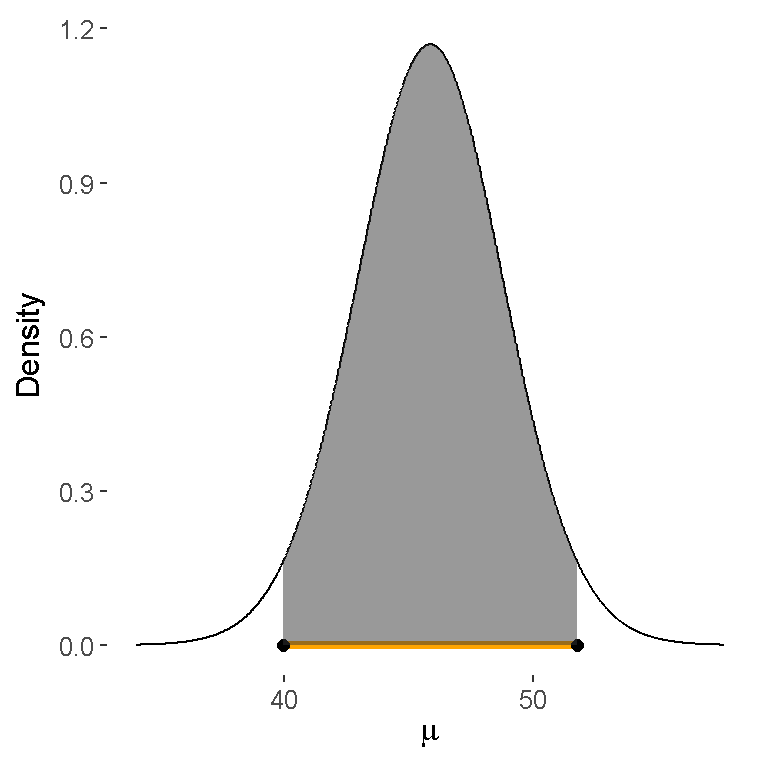
\includegraphics{03-decision-02-normal-gamma_files/figure-latex/tapwater-post-mu-1.pdf}

is the orange interval given by the Lower endpoint L and upper endpoint
U where the probability that mu is in the interval (L, U) is the shaded
area which is equal to zero point nine five.

using the standardized t distribution and some algebra, these values are
\[
\begin{aligned}
  L & =  m_n + t_{0.025}\sqrt{s^2_n/n_n}    \\
  U & =  m_n + t_{0.975}\sqrt{s^2_n/n_n}
\end{aligned}
\] or the posterior mean (our point estimate) plus quantiles of the
standard \(t\) distribution times the scale. Because of the symmetry in
the Student \(t\) distribution, the credible interval is
\(m_n \pm t_{0.975}\sqrt{s^2_n/n_n}\), which should look familiar to
expressions for confidence intervals.

Using the following code in \texttt{R} the 95\% credible interval for
the tap water data is

\begin{Shaded}
\begin{Highlighting}[]
\NormalTok{m_n }\OperatorTok{+}\StringTok{ }\KeywordTok{qt}\NormalTok{(}\KeywordTok{c}\NormalTok{(}\FloatTok{0.025}\NormalTok{, }\FloatTok{0.975}\NormalTok{), v_n)}\OperatorTok{*}\KeywordTok{sqrt}\NormalTok{(s2_n}\OperatorTok{/}\NormalTok{n_n)}
\end{Highlighting}
\end{Shaded}

\begin{verbatim}
## [1] 39.93192 51.75374
\end{verbatim}

Based on the updated posterior, we find that there is a 95 chance that
the mean TTHM concentration is between 39.9 parts per billion and 51.7
parts per billion.

\textbf{Summary} The Normal-Gamma conjugate prior for inference about an
unknown mean and variance for samples from a normal distribution allows
simple expressions for updating prior beliefs given the data. The joint
Normal-Gamma distribution leads to the Student \(t\) distribution for
inference about \(\mu\) when \(\sigma\) is unknown. The Student \(t\)
distribution can be used to provide credible intervals for \(\mu\) using
\texttt{R} or other software that provides quantiles of a standard \(t\)
distribution.

For the energetic learner who is comfortable with calculus, the
following optional material provides more details on how the posterior
distributions were obtained and other results in this section.

For those that are ready to move on, we will introduce Monte Carlo
sampling in the next section; Monte Carlo Sampling is a simulation
method that will allow us to approximate distributions of
transformations of the parameters without using calculus or change of
variables, as well as aid exploratory data analysis of the prior or
posterior distribution.

\textbf{Details of Results (optional reading)}

TBA

\subsection{Monte Carlo Inference}\label{sec:NG-MC}

In this section, we will illustrate Monte Carlo sampling from posterior
distributions and how it can be used for inference. In Section
\ref{sec:normal-gamma}, we can get the posterior distributions for the
precision (inverse variance), and the mean given the precision. Then the
marginal distribution of the mean can be obtained via integration.

Here is a recap of the joint posterior distribution for the mean \(\mu\)
and the precision \(\phi = 1/\sigma^2\):

\begin{itemize}
\tightlist
\item
  Conditional posterior
  \(\mu \mid \data, \sigma^2 \sim \No(m_n, \sigma^2/n_n)\)
\item
  Marginal posterior
  \(1/\sigma^2 = \phi \mid \data \sim \Ga(v_n/2,s^2_n v_n/2)\)
\item
  Marginal posterior \(\mu \mid \data \sim \St(v_n, m_n, s^2_n/n_n)\)
\end{itemize}

What if we are interested in the distribution of the standard deviation
\(\sigma\) itself, or other transformations of the parameters? There may
not be a closed-form expression for the distributions.

However, it turns out that \textbf{Monte Carlo sampling} is an easy way
to make inference, when we cannot analytically calculate distributions
of parameters, expectations, or probabilities. Monte Carlo methods are
computational algorithms that rely on repeated random sampling to
calculate numerical results. The name refers to the famous Monte Carlo
Casino in Monaco, home to games of chance such as Roulette.

Let's start with a case where we know the posterior distribution.

For posterior inference about the precision \(\phi\) using Monte Carlo
simulation, we generate \(S\) random samples from the posterior
distribution:

\[\phi^{(1)},\phi^{(2)},\cdots,\phi^{(S)} \iid \Ga(v_n/2,s^2_n v_n/2)\]

The term \textbf{iid} stands for \textbf{i}ndependent and
\textbf{i}dentically \textbf{d}istributed. In other words, the \(S\)
draws of \(\phi\) are independent and identically distributed from the
gamma distribution.

Then the empirical distribution of the \(S\) samples is used to
approximate the actual posterior distribution. From the samples, the
sample mean of the draws of \(\phi\) can be used to approximate the
posterior mean of \(\phi\).

Likewise, we can calculate probabilities, quantiles and other functions
using the samples from the posterior distribution. For example, if we
want to calculate the posterior expectation of some function of
\(\phi\), written as \(g(\phi)\), we can approximate that by taking the
average of the function, and evaluate it at the \(S\) draws of \(\phi\),
written as \(\frac{1}{S}\sum^S_{i=1}g(\phi^{(i)})\).

The approximation improves as the size of the Monte Carlo simulation
\(S\) increases.

\[\frac{1}{S}\sum^S_{i=1}g(\phi^{(i)}) \rightarrow E(g(\phi \mid \data))\]

\textbf{Example}

We will apply this with the tap water example. To start, we will set a
random seed, which allows the results to be replicated. To generate
1,000 draws from the gamma posterior distribution, we use the
\texttt{rgamma} function \texttt{R} with the posterior hyperparameters
from last time.

\begin{Shaded}
\begin{Highlighting}[]
\KeywordTok{set.seed}\NormalTok{(}\DecValTok{8675309}\NormalTok{)}
\NormalTok{phi =}\StringTok{ }\KeywordTok{rgamma}\NormalTok{(}\DecValTok{1000}\NormalTok{, }\DataTypeTok{shape =}\NormalTok{ v_n}\OperatorTok{/}\DecValTok{2}\NormalTok{, }\DataTypeTok{rate=}\NormalTok{s2_n}\OperatorTok{*}\NormalTok{v_n}\OperatorTok{/}\DecValTok{2}\NormalTok{)}
\end{Highlighting}
\end{Shaded}

Figure \ref{fig:phi-plot} shows the histogram of the 1,000 draws of
\(\phi\) generated from the Monte Carlo simulation, representing the
empirical distribution. The orange line represents the actual gamma
posterior density.

\begin{figure}

{\centering 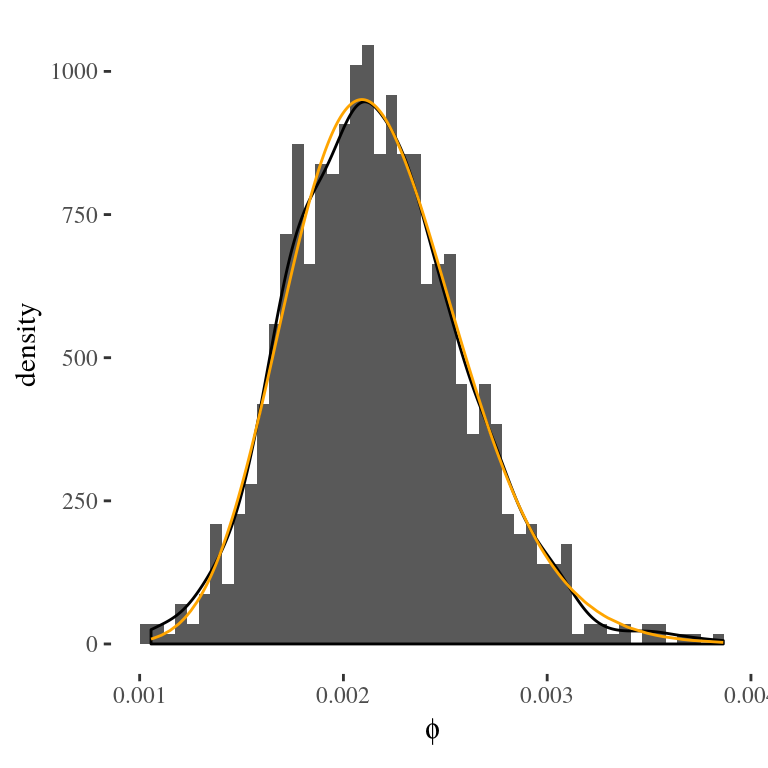
\includegraphics{03-decision-02-normal-gamma_files/figure-latex/phi-plot-1} 

}

\caption{Empirical distribution of the tap water example}\label{fig:phi-plot}
\end{figure}

Try changing the random seed or increasing the number of simulations,
and see how the approximation changes.

We will now use Monte Carlo simulations to approximate the distribution
of \(\sigma\). Since \(\sigma = 1/\sqrt{\phi}\), we can apply the
transformation to the 1,000 draws of \(\phi\) to obtain a random sample
of \(\sigma\). We can then estimate the posterior mean of \(\sigma\) by
calculating the sample mean of the 1,000 draws.

\begin{Shaded}
\begin{Highlighting}[]
\NormalTok{sigma =}\StringTok{ }\DecValTok{1}\OperatorTok{/}\KeywordTok{sqrt}\NormalTok{(phi)}
\KeywordTok{mean}\NormalTok{(sigma) }\CommentTok{# posterior mean of sigma}
\end{Highlighting}
\end{Shaded}

\begin{verbatim}
## [1] 21.81346
\end{verbatim}

Similarly, we can obtain a 95\% credible interval for \(\sigma\) by
finding the sample quantiles of the distribution.

\begin{Shaded}
\begin{Highlighting}[]
\KeywordTok{quantile}\NormalTok{(sigma, }\KeywordTok{c}\NormalTok{(}\FloatTok{0.025}\NormalTok{, }\FloatTok{0.975}\NormalTok{))}
\end{Highlighting}
\end{Shaded}

\begin{verbatim}
##     2.5%    97.5% 
## 18.20655 26.53671
\end{verbatim}

\textbf{Summary}

To recap, we have introduced the powerful method of Monte Carlo
simulation for posterior inference. Monte Carlo methods provide
estimates of expectations, probabilities, and quantiles of distributions
from the simulated values. Monte Carlo simulation also allows us to
approximate distributions of functions of the parameters, or the
transformations of the parameters.

Next we will discuss predictive distributions and show how Monte Carlo
simulation may be used to help choose prior hyperparameters, using the
prior predictive distribution of data.

\subsection{Predictive Distributions}\label{sec:NG-predictive}

In this section, we will discuss prior and posterior \textbf{predictive}
distributions of the data and show how Monte Carlo sampling from the
prior predictive distribution can help select hyper parameters.

We can obtain the prior predictive distribution of the data, by taking
the joint distribution of the data and the parameters in averaging over
the possible values of the parameters from the prior.

\begin{itemize}
\tightlist
\item
  Prior:
\end{itemize}

\[ \begin{aligned}
\frac{1}{\sigma^2} = \phi &\sim \textsf{Gamma}\left(\frac{v_0}{2}, \frac{v_0 s^2_0}{2} \right) \\
\mu \mid \sigma^2  &\sim  \textsf{N}(m_0, \sigma^2/n_0)
\end{aligned} \]

\begin{itemize}
\tightlist
\item
  Sampling model:
\end{itemize}

\[Y_i \mid \mu,\sigma^2 \iid \No(\mu, \sigma^2) \]

\begin{itemize}
\tightlist
\item
  Prior predictive distribution for \(Y\):
\end{itemize}

\[\begin{aligned}
p(Y) &= \iint p(Y \mid \mu,\sigma^2) p(\mu \mid \sigma^2) p(\sigma^2) d\mu \, d\sigma^2 \\
Y &\sim t(v_0, m_0, s_0^2+s_0^2/n_0)
\end{aligned}\]

This distribution of the observables can be used to help elicit prior
hyper parameters as in the tap water example.

A report from the city water department suggests that levels of TTHM are
expected to be between 10-60 parts per billion (ppb).

\begin{itemize}
\item
  Set the prior mean \(\mu\) to be at the midpoint of the interval:
  \(m_0 = (60+10)/2 = 35\)
\item
  Standard deviation: Based on the empirical rule, 95\% observations are
  within \(\pm 2\sigma\) of \(\mu\), we expect that the range of the
  data should be \(4\sigma\).
\item
  Prior estimate of sigma: \(s_0 = (60-10)/4 = 12.5\) or
  \(s_0^2 = [(60-10)/4]^2 = 156.25\)
\end{itemize}

To complete the specification, we also need to choose the prior sample
size \(n_0\) and degrees of freedom \(v_0\). As the degrees of freedom
of the variance are \(n-1\), we set \(v_0 = n_0 - 1\). We will draw
samples from the prior predictive distribution and modify \(n_0\) so
that the simulated data agree with our prior assumptions.

The following \texttt{R} code shows a simulation from the predictive
distribution with the prior sample size of 2. Please note that the
number of Monte Carlo simulations should not be confused with the prior
sample size \(n_0\).

We begin by simulating \(\phi\), transfering \(\phi\) to calculate
\(\sigma\), and then simulating values of \(\mu\). Finally, the
simulated values of \(\mu,\sigma\) are used to generate possible values
of TTHM denoted by \(Y\).

\begin{Shaded}
\begin{Highlighting}[]
\NormalTok{m_}\DecValTok{0}\NormalTok{ =}\StringTok{ }\NormalTok{(}\DecValTok{60}\OperatorTok{+}\DecValTok{10}\NormalTok{)}\OperatorTok{/}\DecValTok{2}\NormalTok{; s2_}\DecValTok{0}\NormalTok{ =}\StringTok{ }\NormalTok{((}\DecValTok{60}\OperatorTok{-}\DecValTok{10}\NormalTok{)}\OperatorTok{/}\DecValTok{4}\NormalTok{)}\OperatorTok{^}\DecValTok{2}\NormalTok{;}
\NormalTok{n_}\DecValTok{0}\NormalTok{ =}\StringTok{ }\DecValTok{2}\NormalTok{; v_}\DecValTok{0}\NormalTok{ =}\StringTok{ }\NormalTok{n_}\DecValTok{0} \OperatorTok{-}\StringTok{ }\DecValTok{1}
\KeywordTok{set.seed}\NormalTok{(}\DecValTok{1234}\NormalTok{)}
\NormalTok{phi =}\StringTok{ }\KeywordTok{rgamma}\NormalTok{(}\DecValTok{10000}\NormalTok{, v_}\DecValTok{0}\OperatorTok{/}\DecValTok{2}\NormalTok{, s2_}\DecValTok{0}\OperatorTok{*}\NormalTok{v_}\DecValTok{0}\OperatorTok{/}\DecValTok{2}\NormalTok{)}
\NormalTok{sigma =}\StringTok{ }\DecValTok{1}\OperatorTok{/}\KeywordTok{sqrt}\NormalTok{(phi)}
\NormalTok{mu =}\StringTok{ }\KeywordTok{rnorm}\NormalTok{(}\DecValTok{10000}\NormalTok{, }\DataTypeTok{mean=}\NormalTok{m_}\DecValTok{0}\NormalTok{, }\DataTypeTok{sd=}\NormalTok{sigma}\OperatorTok{/}\NormalTok{(}\KeywordTok{sqrt}\NormalTok{(n_}\DecValTok{0}\NormalTok{)))}
\NormalTok{y =}\StringTok{ }\KeywordTok{rnorm}\NormalTok{(}\DecValTok{10000}\NormalTok{, mu, sigma)}
\KeywordTok{quantile}\NormalTok{(y, }\KeywordTok{c}\NormalTok{(}\FloatTok{0.025}\NormalTok{,}\FloatTok{0.975}\NormalTok{))}
\end{Highlighting}
\end{Shaded}

\begin{verbatim}
##      2.5%     97.5% 
## -140.1391  217.7050
\end{verbatim}

This forward simulation propagates uncertainty in \(\mu,\sigma\) to the
prior predictive distribution of the data. Calculating the sample
quantiles from the samples of the prior predictive for \(Y\), we see
that the 95\% predictive interval includes negative values. Since TTHM
is non-negative, we need to adjust \(n_0\) and repeat.

After some trial and error, we find that the prior sample size of 25 (in
fact the Central Limit Theorem suggests at least 25 or 30 to be
``sufficiently large''), the empirical quantiles from the prior
predictive distribution are close to the range of 10 to 16 that we were
given as prior information.

\begin{Shaded}
\begin{Highlighting}[]
\NormalTok{m_}\DecValTok{0}\NormalTok{ =}\StringTok{ }\NormalTok{(}\DecValTok{60}\OperatorTok{+}\DecValTok{10}\NormalTok{)}\OperatorTok{/}\DecValTok{2}\NormalTok{; s2_}\DecValTok{0}\NormalTok{ =}\StringTok{ }\NormalTok{((}\DecValTok{60}\OperatorTok{-}\DecValTok{10}\NormalTok{)}\OperatorTok{/}\DecValTok{4}\NormalTok{)}\OperatorTok{^}\DecValTok{2}\NormalTok{;}
\NormalTok{n_}\DecValTok{0}\NormalTok{ =}\StringTok{ }\DecValTok{25}\NormalTok{; v_}\DecValTok{0}\NormalTok{ =}\StringTok{ }\NormalTok{n_}\DecValTok{0} \OperatorTok{-}\StringTok{ }\DecValTok{1}
\KeywordTok{set.seed}\NormalTok{(}\DecValTok{1234}\NormalTok{)}
\NormalTok{phi =}\StringTok{ }\KeywordTok{rgamma}\NormalTok{(}\DecValTok{10000}\NormalTok{, v_}\DecValTok{0}\OperatorTok{/}\DecValTok{2}\NormalTok{, s2_}\DecValTok{0}\OperatorTok{*}\NormalTok{v_}\DecValTok{0}\OperatorTok{/}\DecValTok{2}\NormalTok{)}
\NormalTok{sigma =}\StringTok{ }\DecValTok{1}\OperatorTok{/}\KeywordTok{sqrt}\NormalTok{(phi)}
\NormalTok{mu =}\StringTok{ }\KeywordTok{rnorm}\NormalTok{(}\DecValTok{10000}\NormalTok{, }\DataTypeTok{mean=}\NormalTok{m_}\DecValTok{0}\NormalTok{, }\DataTypeTok{sd=}\NormalTok{sigma}\OperatorTok{/}\NormalTok{(}\KeywordTok{sqrt}\NormalTok{(n_}\DecValTok{0}\NormalTok{)))}
\NormalTok{y =}\StringTok{ }\KeywordTok{rnorm}\NormalTok{(}\DecValTok{10000}\NormalTok{, mu, sigma)}
\KeywordTok{quantile}\NormalTok{(y, }\KeywordTok{c}\NormalTok{(}\FloatTok{0.025}\NormalTok{,}\FloatTok{0.975}\NormalTok{))}
\end{Highlighting}
\end{Shaded}

\begin{verbatim}
##      2.5%     97.5% 
##  8.802515 61.857350
\end{verbatim}

Figure \ref{fig:hist-prior} shows an estimate of the prior distribution
of \(\mu\) in gray and the more dispersed prior predictive distribution
in TTHM in orange, obtained from the Monte Carlo samples.

\begin{figure}

{\centering 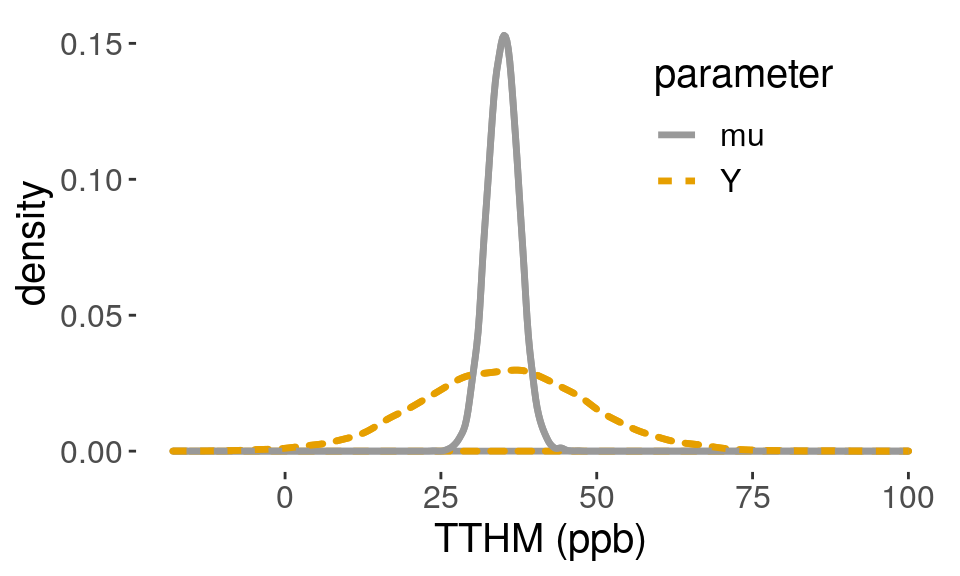
\includegraphics{03-decision-02-normal-gamma_files/figure-latex/hist-prior-1} 

}

\caption{Prior density}\label{fig:hist-prior}
\end{figure}

Using the Monte Carlo samples, we can also estimate the prior
probability of negative values of TTHM by counting the number of times
the simulated values are less than zero out of the total number of
simulations.

\begin{Shaded}
\begin{Highlighting}[]
\KeywordTok{sum}\NormalTok{(y }\OperatorTok{<}\StringTok{ }\DecValTok{0}\NormalTok{)}\OperatorTok{/}\KeywordTok{length}\NormalTok{(y)  }\CommentTok{# P(Y < 0) a priori}
\end{Highlighting}
\end{Shaded}

\begin{verbatim}
## [1] 0.0049
\end{verbatim}

With the normal prior distribution, this probability will never be zero,
but may be acceptably small, so we can still use the conjugate normal
gamma model for analysis.

We can use the same strategy to generate samples from the predictive
distribution of a new measurement \(Y_{n+1}\) given the observed data.
In mathematical terms, the posterior predictive distribution is written
as

\[Y_{n+1} \mid Y_1, \ldots, Y_n \sim \St(v_n, m_n, s^2_n (1 + 1/n_n))\]

In the code, we replace the prior hyper parameters with the posterior
hyper parameters from last time.

\begin{Shaded}
\begin{Highlighting}[]
\KeywordTok{set.seed}\NormalTok{(}\DecValTok{1234}\NormalTok{)}
\NormalTok{phi =}\StringTok{ }\KeywordTok{rgamma}\NormalTok{(}\DecValTok{10000}\NormalTok{, v_n}\OperatorTok{/}\DecValTok{2}\NormalTok{, s2_n}\OperatorTok{*}\NormalTok{v_n}\OperatorTok{/}\DecValTok{2}\NormalTok{)}
\NormalTok{sigma =}\StringTok{ }\DecValTok{1}\OperatorTok{/}\KeywordTok{sqrt}\NormalTok{(phi)}
\NormalTok{post_mu =}\StringTok{ }\KeywordTok{rnorm}\NormalTok{(}\DecValTok{10000}\NormalTok{, }\DataTypeTok{mean=}\NormalTok{m_n, }\DataTypeTok{sd=}\NormalTok{sigma}\OperatorTok{/}\NormalTok{(}\KeywordTok{sqrt}\NormalTok{(n_n)))}
\NormalTok{pred_y =}\StringTok{  }\KeywordTok{rnorm}\NormalTok{(}\DecValTok{10000}\NormalTok{,post_mu, sigma)}
\KeywordTok{quantile}\NormalTok{(pred_y, }\KeywordTok{c}\NormalTok{(.}\DecValTok{025}\NormalTok{, .}\DecValTok{975}\NormalTok{))}
\end{Highlighting}
\end{Shaded}

\begin{verbatim}
##      2.5%     97.5% 
##  3.324087 89.871964
\end{verbatim}

Figure \ref{fig:hist-pred} shows the Monte Carlo approximation to the
prior distribution of \(\mu\), and the posterior distribution of \(\mu\)
which is shifted to the right. The prior and posterior predictive
distributions are also depicted, showing how the data have updated the
prior information.

\begin{figure}

{\centering 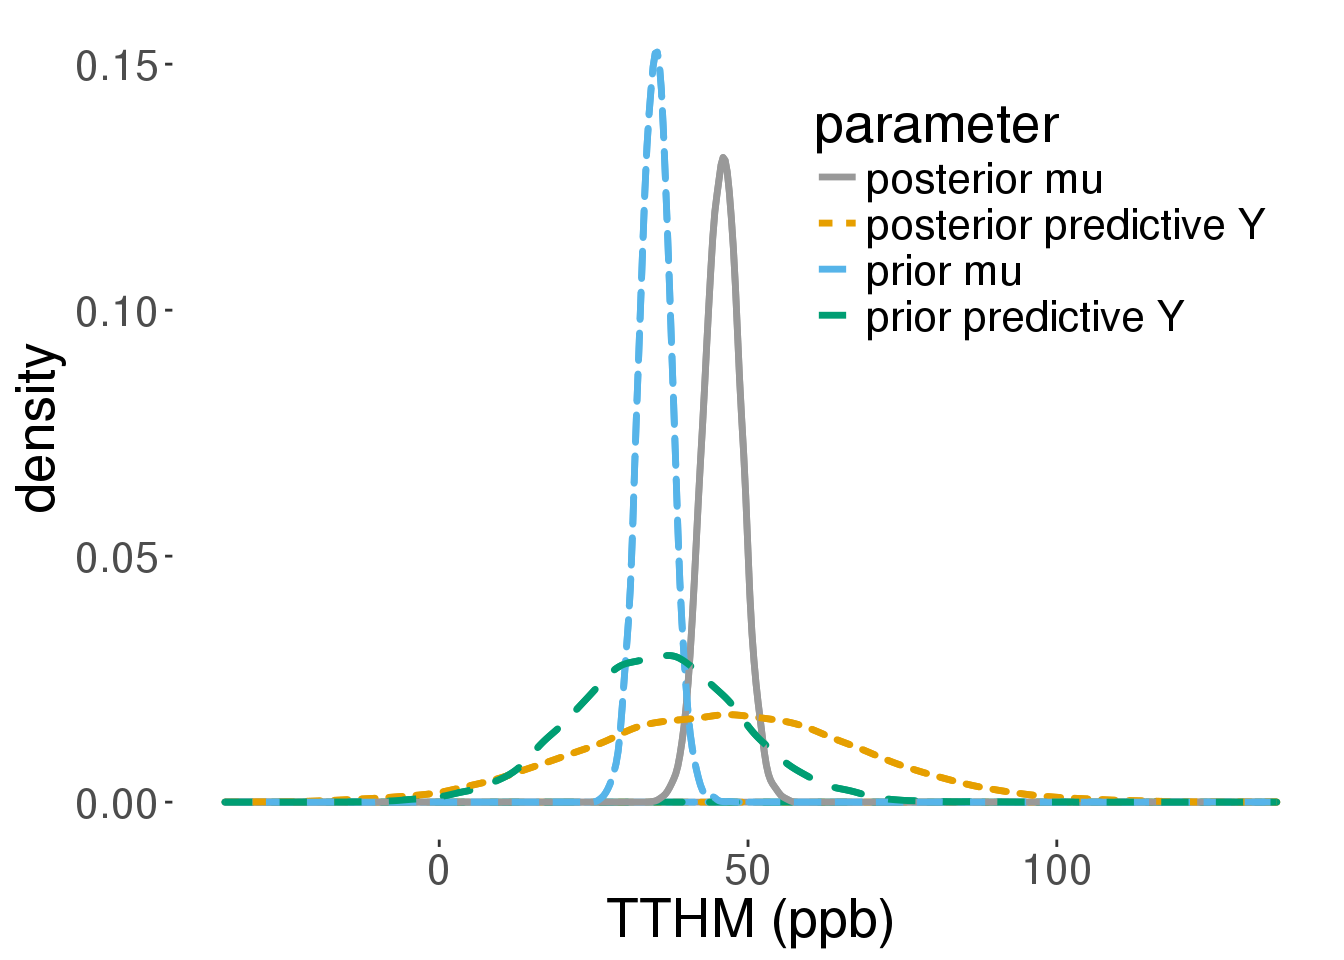
\includegraphics{03-decision-02-normal-gamma_files/figure-latex/hist-pred-1} 

}

\caption{Posterior densities}\label{fig:hist-pred}
\end{figure}

Using the Monte-Carlo samples from the posterior predictive
distribution, we can estimate the probability that a new TTHM sample
will exceed the legal limit of 80 parts per billion, which is
approximately 0.06.

\begin{Shaded}
\begin{Highlighting}[]
\KeywordTok{sum}\NormalTok{(pred_y }\OperatorTok{>}\StringTok{ }\DecValTok{80}\NormalTok{)}\OperatorTok{/}\KeywordTok{length}\NormalTok{(pred_y)  }\CommentTok{# P(Y > 80 | data)}
\end{Highlighting}
\end{Shaded}

\begin{verbatim}
## [1] 0.0623
\end{verbatim}

By using Monte-Carlo methods, we can obtain prior and posterior
predictive distributions of the data.

\begin{itemize}
\item
  Sampling from the prior predictive distribution can help with the
  selection of prior hyper parameters and verify that these choices
  reflect the prior information that is available.
\item
  Visualizing prior predictive distributions based on Monte Carlo
  simulations can help explore implications of our prior assumptions
  such as the choice of the hyper parameters or even assume
  distributions.
\item
  If samples are incompatible with known information, such as support on
  positive values, we may need to modify assumptions and look at other
  families of prior distributions.
\end{itemize}

\subsection{Reference Priors}\label{sec:NG-reference}

In Section \ref{sec:NG-predictive}, we described a way of specifying an
informative prior distribution for inference about TTHM in tapwater
based on additional prior information. We had to use a prior sample size
that was comparable to the observed sample size for the prior predictive
under the Normal-Gamma distribution to agree with the reported prior
interval.

However, there may be cases where prior information is not available, or
you may wish to present an objective analysis where minimal prior
information is used. Or perhaps, you want to use the Bayesian paradigm
to make probability statements about parameters, but not use any prior
information.

In this section, we will present reference priors for normal data, which
can be viewed as a limiting form of the Normal-Gamma conjugate prior
distribution. \textbf{Can you actually perform a Bayesian analysis
without using prior information?}

Conjugate priors can be interpreted to be based on a prior sample. What
happens in the conjugate Normal-Gamma prior if we take our prior sample
size \(n_0\) to go to zero? If we have no data, then we will define the
prior sample variance \(s_0^2\) to go to 0, and based on the
relationship between prior sample sized and prior degrees of freedom, we
will let the prior degrees of freedom go to the prior sample size minus
one, or negative 1, i.e. \(v_0 = n_0 - 1 \rightarrow -1\).

With this limit, we have the following properties:

\begin{itemize}
\item
  The posterior mean goes to the sample mean.
\item
  The posterior sample size is the observed sample size.
\item
  The posterior degrees of freedom go to the sample degrees of freedom.
\item
  The posterior variance parameter goes to the sample variance.
\end{itemize}

In this limit, the posterior hyperparameters do not depend on the prior
hyperparameters.

Since
\(n_0 \rightarrow 0, s^2_0 \rightarrow 0, v_0 = n_0 - 1 \rightarrow -1\),
we have in mathematical terms:

\[\begin{aligned}
m_n &= \frac{n \bar{Y} + n_0 m_0} {n + n_0}  \rightarrow \bar{Y} \\
n_n &= n_0 + n  \rightarrow n \\
v_n &= v_0 + n  \rightarrow n-1 \\
s^2_n &= \frac{1}{v_n}\left[s^2_0 v_0 + s^2 (n-1) + \frac{n_0 n}{n_n} (\bar{Y} - m_0)^2 \right] \rightarrow s^2
\end{aligned}\]

This limiting Normal-gamma distribution, \(\No-\Ga(0,0,0,-1)\), is not
really a normal gamma distribution, as the density does not integrate to
1. The form of the limit can be viewed as a prior for \(\mu\) that is
proportional to a constant, or uniform/flat on the whole real line. And
a prior for the variance is proportional to 1 over the variance. The
joint prior is taken as the product of the two.

\[\begin{aligned}
p(\mu \mid \sigma^2) & \propto  1 \\
p(\sigma^2) & \propto  1/\sigma^2 \\
p(\mu, \sigma^2) & \propto  1/\sigma^2
\end{aligned}\]

This is refered to as a \textbf{reference prior} because the posterior
hyperparameters do not depend on the prior hyperparameters.

In addition, \(\textsf{NormalGamma}(0,0,0,-1)\) is a special case of a
reference prior, known as the independent Jeffreys prior. While Jeffreys
used other arguments to arrive at the form of the prior, the goal was to
have an \textbf{objective prior} invariant to shifting the data by a
constant or multiplying by a constant.

Now, a naive approach to constructing a non-informative distribution
might be to use a uniform distribution to represent lack of knowledge.
However, would you use a uniform distribution for \(\sigma^2\), or a
uniform distribution for the precision \(1/\sigma^2\)? Or perhaps a
uniform distribution for \(\sigma\)? These would all lead to different
posteriors with little justification for any of them. This ambiguity led
Sir Harold Jeffreys to propose reference distributions for the mean and
variance for situations where prior information was limited. These
priors are \textbf{invariant} to the units of the data.

The unnormalized priors that do not integrate to a constant are called
\textbf{improper distributions}. An important consideration in using
them is that one cannot generate samples from the prior or the prior
predictive distribution to data and are referred to as
\textbf{non-generative distributions}.

While the reference prior is not a proper prior distribution, and cannot
reflect anyone's actual prior beliefs, the formal application phase rule
can still be used to show that \textbf{the posterior distribution is a
valid normal gamma distribution}, leading to a formal phase posterior
distribution. That depends only on summary statistics of the data.

The posterior distribution
\(\textsf{NormalGamma}(\bar{Y}, n, s^2, n-1)\) breaks down to

\[\begin{aligned}
\mu \mid \sigma^2, \data & \sim \No(\bar{Y}, \sigma^2/n) \\
1/\sigma^2  \mid \data & \sim \Ga((n-1)/2, s^2(n - 1)/2).
\end{aligned}\]

\begin{itemize}
\tightlist
\item
  Under the reference prior \(p(\mu, \sigma^2) \propto 1/\sigma^2\), the
  posterior distribution after standardizing \(\mu\) has a Student \(t\)
  distribution with n minus one degrees of freedom.
\end{itemize}

\[\frac{\mu - \bar{Y}}{\sqrt{s^2/n}} \mid \data \sim  \St(n-1, 0, 1)\] *
Prior to seeing the data, the distribution of the standardized sample
mean given \(\mu\) and \(\sigma\) also has a Student t distribution.

\[\frac{\mu - \bar{Y}}{\sqrt{s^2/n}} \mid \mu, \sigma^2 \sim  \St(n-1, 0, 1) \]

\begin{itemize}
\tightlist
\item
  Both frequentist sampling distributions and Bayesian reference
  posterior distributions lead to intervals of this form:
\end{itemize}

\[(\bar{Y} - t_{1 - \alpha/2} s/\sqrt{n}, \, \bar{Y} + t_{1 - \alpha/2} s/\sqrt{n})\]

\begin{itemize}
\tightlist
\item
  However, only the Bayesian approach justifies the probability
  statements about \(\mu\) being in the interval after seeing the data.
\end{itemize}

\[P(\bar{Y} - t_{1 - \alpha/2} s/\sqrt{n} < \mu <  \bar{Y} + t_{1 - \alpha/2} s/\sqrt{n}) = 1 - \alpha\]

We can use either analytic expressions based on the t-distribution, or
Monte Carlo samples from the posterior predictive distribution, to make
predictions about a new sample.

Here is some code to generate the Monte Carlo samples from the tap water
example:

\begin{Shaded}
\begin{Highlighting}[]
\NormalTok{phi =}\StringTok{ }\KeywordTok{rgamma}\NormalTok{(}\DecValTok{10000}\NormalTok{, (n}\OperatorTok{-}\DecValTok{1}\NormalTok{)}\OperatorTok{/}\DecValTok{2}\NormalTok{, s2}\OperatorTok{*}\NormalTok{(n}\OperatorTok{-}\DecValTok{1}\NormalTok{)}\OperatorTok{/}\DecValTok{2}\NormalTok{)}
\NormalTok{sigma =}\StringTok{ }\DecValTok{1}\OperatorTok{/}\KeywordTok{sqrt}\NormalTok{(phi)}
\NormalTok{post_mu =}\StringTok{ }\KeywordTok{rnorm}\NormalTok{(}\DecValTok{10000}\NormalTok{, }\DataTypeTok{mean=}\NormalTok{ybar, }\DataTypeTok{sd=}\NormalTok{sigma}\OperatorTok{/}\NormalTok{(}\KeywordTok{sqrt}\NormalTok{(n)))}
\NormalTok{pred_y =}\StringTok{  }\KeywordTok{rnorm}\NormalTok{(}\DecValTok{10000}\NormalTok{,post_mu, sigma)}
\KeywordTok{quantile}\NormalTok{(pred_y, }\KeywordTok{c}\NormalTok{(.}\DecValTok{025}\NormalTok{, .}\DecValTok{975}\NormalTok{))}
\end{Highlighting}
\end{Shaded}

\begin{verbatim}
##       2.5%      97.5% 
##   6.692877 104.225954
\end{verbatim}

Using the Monte Carlo samples, Figure \ref{fig:plot-post-pred} shows the
posterior distribution based on the informative Normal-Gamma prior and
the reference prior. Both the posterior distribution for \(\mu\) and the
posterior predictive distribution for a new sample are shifted to the
right, and are centered at the sample mean. The posterior for \(\mu\)
under the reference prior is less concentrated around its mean than the
posterior under the informative prior, which leads to an increased
posterior sample size and hence increased precision.

\begin{figure}

{\centering 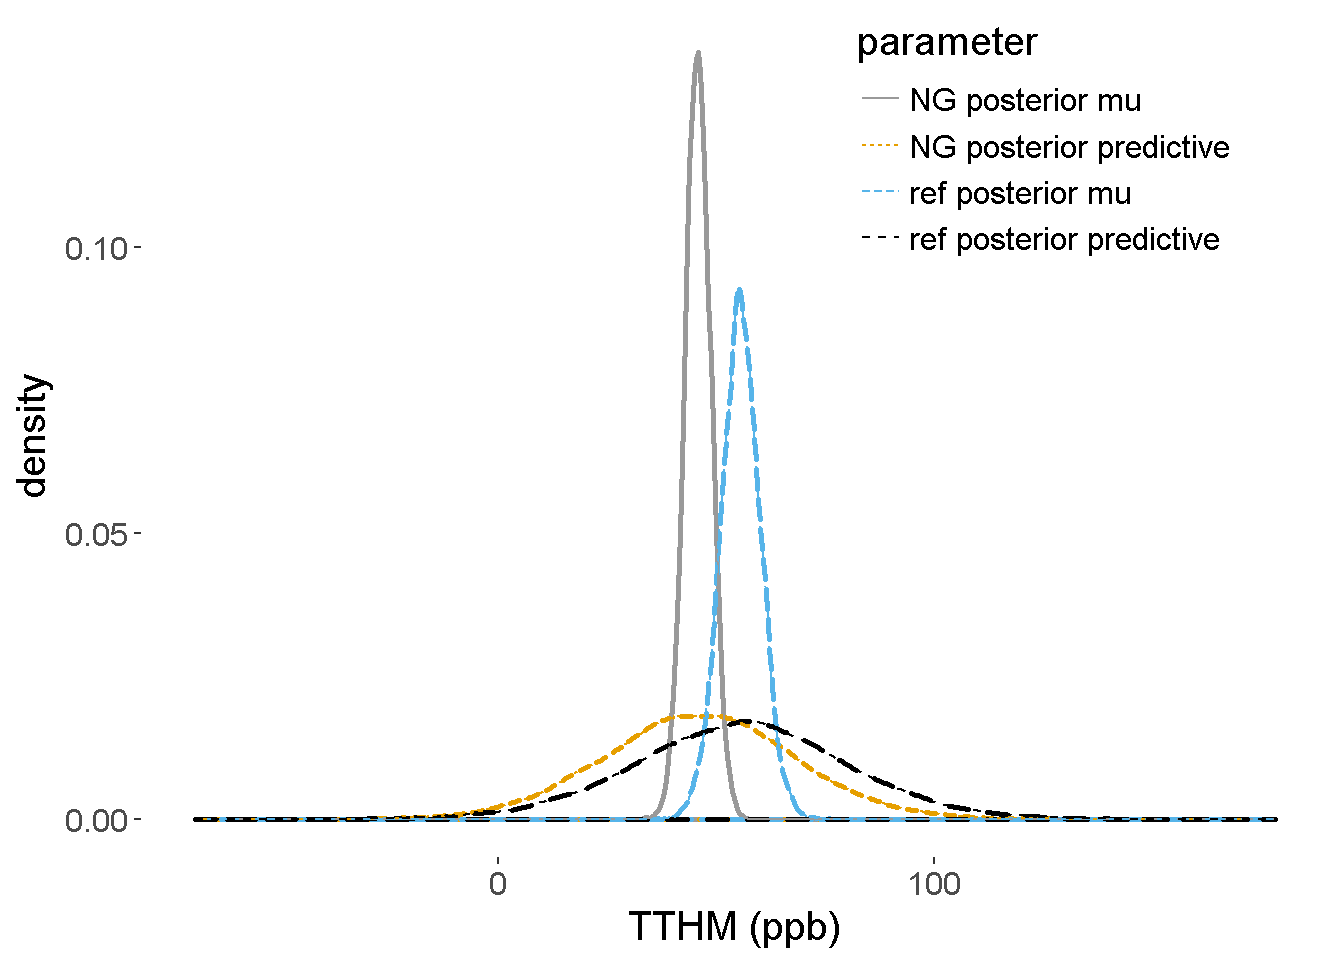
\includegraphics{03-decision-02-normal-gamma_files/figure-latex/plot-post-pred-1} 

}

\caption{Comparison of posterior densities}\label{fig:plot-post-pred}
\end{figure}

The posterior probability that a new sample will exceed the legal limit
of 80 ppb under the reference prior is roughly 0.15, which is more than
double the probability of 0.06 from the posterior under the informative
prior.

\begin{Shaded}
\begin{Highlighting}[]
\KeywordTok{sum}\NormalTok{(pred_y }\OperatorTok{>}\StringTok{ }\DecValTok{80}\NormalTok{)}\OperatorTok{/}\KeywordTok{length}\NormalTok{(pred_y)  }\CommentTok{# P(Y > 80 | data)}
\end{Highlighting}
\end{Shaded}

\begin{verbatim}
## [1] 0.1534
\end{verbatim}

In constructing the informative prior from the reported interval, there
are two critical assumptions. First, the prior data are exchangeable
with the observed data. Second, the conjugate normal gamma distribution
is suitable for representing the prior information. These assumptions
may or may not be verifiable, but they should be considered carefully
when using informative conjugate priors.

In the case of the tap water example, there are several concerns: One,
it is unclear that the prior data are exchangeable with the observed
data. For example, water treatment conditions may have changed. Two, the
prior sample size was not based on a real prior sample, but instead
selected so that the prior predictive intervals under the normal gamma
model agreed with the prior data. As we do not have access to the prior
data, we cannot check assumptions about normality that would help
justify the prior. Other skewed distributions may be consistent with the
prior interval, but lead to different conclusions.

To recap, we have introduced a reference prior for inference for normal
data with an unknown mean and variance. Reference priors are often part
of a prior sensitivity study and are used when objectivity is of utmost
importance.

If conclusions are fundamentally different with an informative prior and
a reference prior, one may wish to carefully examine assumputions that
led to the informative prior.

\begin{itemize}
\item
  Is the prior information based on a prior sample that is exchangable
  with the observed data?
\item
  Is the normal-gamma assumption appropriate?
\end{itemize}

Informative priors can provide more accurate inference when data are
limited, and the transparency of explicitly laying out prior assumptions
is an important aspect of reproducible research. However, one needs to
be careful that certain prior assumptions may lead to un-intended
consequences.

Next, we will investigate a prior distribution that is a mixture of
conjugate priors, so the new prior distribution provides robustness to
prior mis-specification in the prior sample size.

While we will no longer have nice analytical expressions for the
posterior, we can simulate from the posterior distribution using a Monte
Carlo algorithm called Markov chain Monte Carlo (MCMC).

\subsection{Mixtures of Conjugate Priors}\label{sec:NG-Cauchy}

In this section, we will describe priors that are constructed as a
mixture of conjugate priors -- in particular, the Cauchy distribution.
As these are no longer conjugate priors, nice analytic expressions for
the posterior distribution are not available. However, we can use a
Monte Carlo algorithm called Markov chain Monte Carlo (MCMC) for
posterior inference.

In many situations, we may have reasonable prior information about the
mean \(\mu\), but we are less confident in how many observations our
prior beliefs are equivalent to. We can address this uncertainty in the
prior sample size, through an additional prior distribution on a \(n_0\)
via a hierarchical prior.

The hierarchical prior for the normal gamma distribution is written as
\[\begin{aligned}
\mu \mid \sigma^2, n_0 & \sim \No(m_0, \sigma^2/n_0) \\
n_0 \mid \sigma^2 &  \sim \Ga(1/2, r^2/2)
\end{aligned}\]

If \(r=1\), then this corresponds to a prior expected sample size of one
because the expectation of \(\Ga(1/2,1/2)\) is one.

The marginal prior distribution from \(\mu\) can be attained via
integration, and we get

\[\mu \mid \sigma^2  \sim  \Ca(m_0, \sigma^2 r^2)\]

This is a \textbf{Cauchy distribution} centered at the prior mean
\(m_0\), with the scale parameter \(\sigma^2 r^2\).

\subsection{MCMC}\label{sec:NG-MCMC}

\section{Hypothesis Testing with Normal
Populations}\label{hypothesis-testing-with-normal-populations}

\subsection{Bayes Factors for Testing a Normal Mean: variance
known}\label{bayes-factors-for-testing-a-normal-mean-variance-known}

\subsection{Bayes Factors for Testing a Normal Mean: unknown
variance}\label{bayes-factors-for-testing-a-normal-mean-unknown-variance}

\subsection{Testing Normal Means: paired
data}\label{testing-normal-means-paired-data}

\subsection{Testing Normal Means: independent
groups}\label{testing-normal-means-independent-groups}

\subsection{Inference after Testing}\label{inference-after-testing}

\section{Exercises}\label{exercises-1}

Test something here

\chapter{Introduction to Bayesian
Regression}\label{introduction-to-bayesian-regression}

In the previous chapter, we introduced Bayesian decision making using
posterior probabilities and a variety of loss functions. We discussed
how to minimize the expected loss for hypothesis testing. Moreover, we
instroduce the concept of Bayes factors and gave some examples of how
they can be used in Bayesian hypothesis testing for comparison of two
means. We also discussed how to choose appropriate and robust priors.
When there is no conjugacy, we applied Markov Chain Monte Carlo
simulation to approximate the posterior distributions of parameters of
interest.

In this chapter, we will apply Bayesian inference to linear regression.
We will first apply Bayesian statistics to simple linear regression
models, then generalize the results to multiple linear regression
models. We will see when using the reference prior, the posterior means,
posterior standard deviations, and credible intervals of the
coefficients will coincide with the counterparts in the frequentist
ordinary least square (OLS) linear regression models. However, using the
Bayes framework, we can now interpret the credible intervals as the
probability of the coefficients lie in such intervals.

\section{Bayesian Simple Linear
Regression}\label{bayesian-simple-linear-regression}

In this section, we turn to Bayesian inference in simple linear
regression. We will use reference prior distribution which will provide
a connection between the frequentist solution and Bayesian answers. This
provides a baseline analysis for comparions with more informative prior
distributions. To illustrate the ideas, we will use an example of
predicting body fat.

\subsection{Frequentist Ordinary Least Square Simple Linear
Regression}\label{frequentist-ordinary-least-square-simple-linear-regression}

Obtaining accurate measurements of body fat is expensive and not easy to
be done. Instaed, predictive models which predict the percentage of body
fat using readily available measurements such as abdominal circumference
are easy to use and inexpensive. We will illustrate this using the
\texttt{bodyfat} data from the library \texttt{BAS}.

To start, we load the \texttt{BAS} library (you may download the package
from CRAN) to access the dataframe. We print out a summary of the
variables in this dataframe.

\begin{Shaded}
\begin{Highlighting}[]
\KeywordTok{library}\NormalTok{(BAS)}
\end{Highlighting}
\end{Shaded}

\begin{verbatim}
## Warning: package 'BAS' was built under R version 3.4.2
\end{verbatim}

\begin{Shaded}
\begin{Highlighting}[]
\KeywordTok{data}\NormalTok{(bodyfat)}
\KeywordTok{summary}\NormalTok{(bodyfat)}
\end{Highlighting}
\end{Shaded}

\begin{verbatim}
##     Density         Bodyfat           Age            Weight     
##  Min.   :0.995   Min.   : 0.00   Min.   :22.00   Min.   :118.5  
##  1st Qu.:1.041   1st Qu.:12.47   1st Qu.:35.75   1st Qu.:159.0  
##  Median :1.055   Median :19.20   Median :43.00   Median :176.5  
##  Mean   :1.056   Mean   :19.15   Mean   :44.88   Mean   :178.9  
##  3rd Qu.:1.070   3rd Qu.:25.30   3rd Qu.:54.00   3rd Qu.:197.0  
##  Max.   :1.109   Max.   :47.50   Max.   :81.00   Max.   :363.1  
##      Height           Neck           Chest           Abdomen      
##  Min.   :29.50   Min.   :31.10   Min.   : 79.30   Min.   : 69.40  
##  1st Qu.:68.25   1st Qu.:36.40   1st Qu.: 94.35   1st Qu.: 84.58  
##  Median :70.00   Median :38.00   Median : 99.65   Median : 90.95  
##  Mean   :70.15   Mean   :37.99   Mean   :100.82   Mean   : 92.56  
##  3rd Qu.:72.25   3rd Qu.:39.42   3rd Qu.:105.38   3rd Qu.: 99.33  
##  Max.   :77.75   Max.   :51.20   Max.   :136.20   Max.   :148.10  
##       Hip            Thigh            Knee           Ankle     
##  Min.   : 85.0   Min.   :47.20   Min.   :33.00   Min.   :19.1  
##  1st Qu.: 95.5   1st Qu.:56.00   1st Qu.:36.98   1st Qu.:22.0  
##  Median : 99.3   Median :59.00   Median :38.50   Median :22.8  
##  Mean   : 99.9   Mean   :59.41   Mean   :38.59   Mean   :23.1  
##  3rd Qu.:103.5   3rd Qu.:62.35   3rd Qu.:39.92   3rd Qu.:24.0  
##  Max.   :147.7   Max.   :87.30   Max.   :49.10   Max.   :33.9  
##      Biceps         Forearm          Wrist      
##  Min.   :24.80   Min.   :21.00   Min.   :15.80  
##  1st Qu.:30.20   1st Qu.:27.30   1st Qu.:17.60  
##  Median :32.05   Median :28.70   Median :18.30  
##  Mean   :32.27   Mean   :28.66   Mean   :18.23  
##  3rd Qu.:34.33   3rd Qu.:30.00   3rd Qu.:18.80  
##  Max.   :45.00   Max.   :34.90   Max.   :21.40
\end{verbatim}

This dataframe includes 252 measurements on men of body fat and other
measurements, such as waist circumference (\texttt{Abdomen}). We will
use \texttt{Abdomen} to illustrate Bayesian simple linear regression. We
regress the response variable \texttt{Bodyfat} on the predictor
\texttt{Abdomen}, which gives us the model
\[ Y_i = \alpha + \beta X_i + \epsilon_i, \] which the assumption that
the errors \(\epsilon_i\) are independent and identically distributed as
normal random variables with mean zero and constant variance
\(\sigma^2\).

The figure below shows the percentage body fat obtained from under water
weighing and the abdominal circumference for 252 men. To predict body
fat, the line overlayed on the scatter plot illustrates the best fitting
ordinary least squares line obtained with the \texttt{lm} function in R.

\begin{Shaded}
\begin{Highlighting}[]
\KeywordTok{plot}\NormalTok{(Bodyfat }\OperatorTok{~}\StringTok{ }\NormalTok{Abdomen, }\DataTypeTok{data =}\NormalTok{ bodyfat, }
     \DataTypeTok{xlab =} \StringTok{"abdomen circumference (cm)"}\NormalTok{, }
     \DataTypeTok{col =} \StringTok{"blue"}\NormalTok{, }\DataTypeTok{pch =} \DecValTok{16}\NormalTok{, }\DataTypeTok{main =} \StringTok{""}\NormalTok{)}

\CommentTok{# Ordinary least square linear regression}
\NormalTok{bodyfat.lm =}\StringTok{ }\KeywordTok{lm}\NormalTok{(Bodyfat }\OperatorTok{~}\StringTok{ }\NormalTok{Abdomen, }\DataTypeTok{data =}\NormalTok{ bodyfat)}
\KeywordTok{summary}\NormalTok{(bodyfat.lm)}
\end{Highlighting}
\end{Shaded}

\begin{verbatim}
## 
## Call:
## lm(formula = Bodyfat ~ Abdomen, data = bodyfat)
## 
## Residuals:
##      Min       1Q   Median       3Q      Max 
## -19.0160  -3.7557   0.0554   3.4215  12.9007 
## 
## Coefficients:
##              Estimate Std. Error t value Pr(>|t|)    
## (Intercept) -39.28018    2.66034  -14.77   <2e-16 ***
## Abdomen       0.63130    0.02855   22.11   <2e-16 ***
## ---
## Signif. codes:  0 '***' 0.001 '**' 0.01 '*' 0.05 '.' 0.1 ' ' 1
## 
## Residual standard error: 4.877 on 250 degrees of freedom
## Multiple R-squared:  0.6617, Adjusted R-squared:  0.6603 
## F-statistic: 488.9 on 1 and 250 DF,  p-value: < 2.2e-16
\end{verbatim}

\begin{Shaded}
\begin{Highlighting}[]
\NormalTok{beta =}\StringTok{ }\KeywordTok{coef}\NormalTok{(bodyfat.lm)}
\KeywordTok{abline}\NormalTok{(beta, }\DataTypeTok{lwd =} \DecValTok{4}\NormalTok{, }\DataTypeTok{col =} \DecValTok{1}\NormalTok{)}
\end{Highlighting}
\end{Shaded}

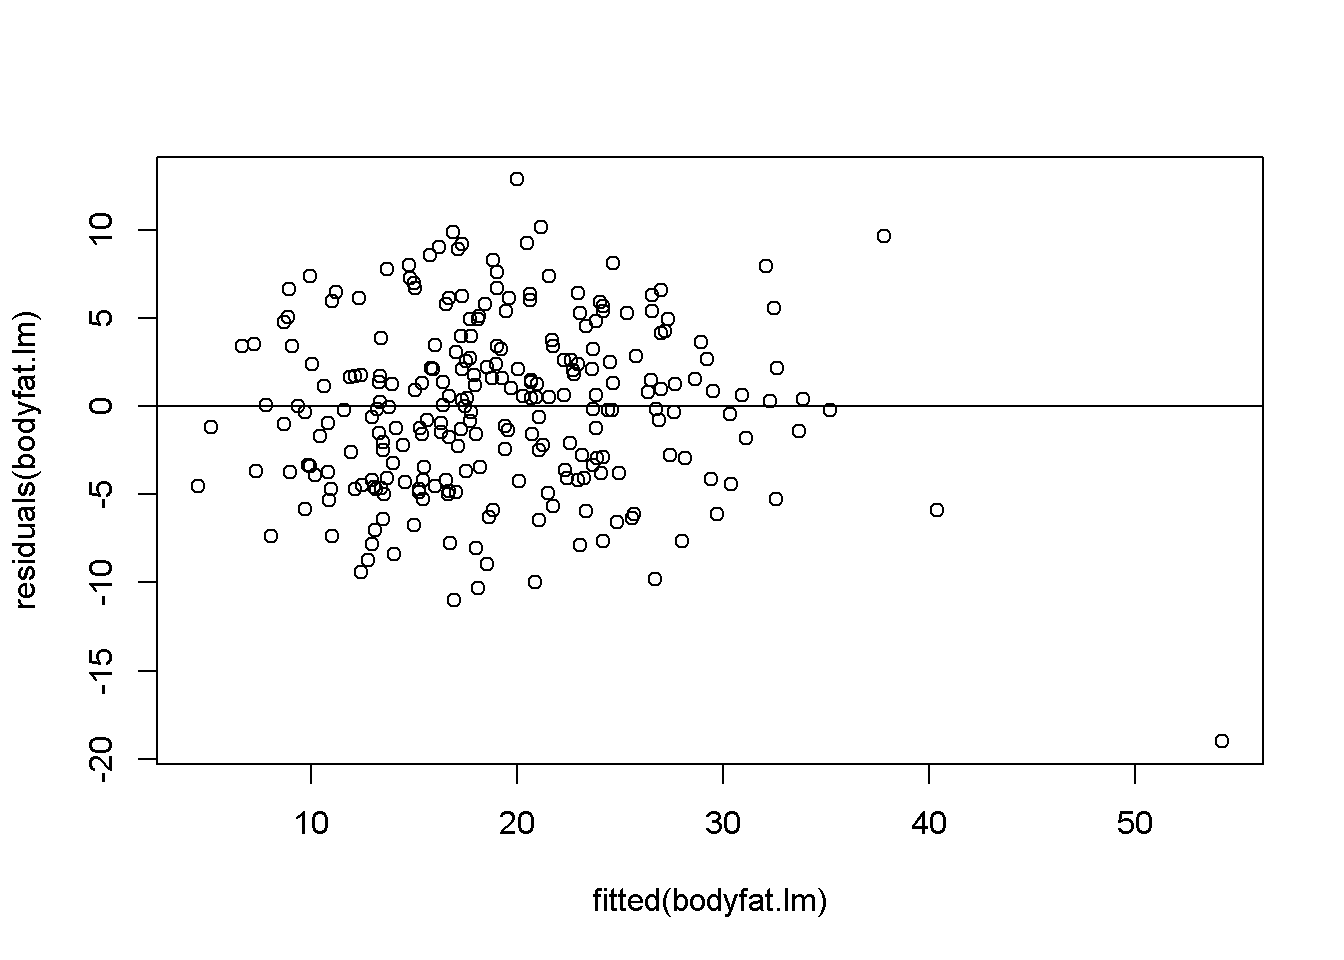
\includegraphics{04-regression-01-Bayesian-simple-regression_files/figure-latex/unnamed-chunk-2-1.pdf}

From the summary, we see that this model has an estimated slope,
\(\hat{\beta}\), of 0.63 and an estimated intercept, \(\hat{\alpha}\),
of about -39.28\%. For every additional centimeter, we expect body fat
to increase by 0.63\%. The negative interceptive course does not make
sense as a physical model, but neither does predicting a male with a
waist of zero centimeters. Nevertheless, this linear regression may be
an accurate approximation for prediction purposes for measurements that
are in the observed range for this population.

The residuals, which provide an estimate of the fitting error, are equal
to \(\hat{\epsilon}_i = Y_i - \hat{Y}_i\), the difference between the
observed values \(Y_i\) and the fited values
\(\hat{Y}_i = \hat{\alpha} + \hat{\beta}X_i\), where \(X_i\) is the
abdominal circumference for the \(i\)th male. \(\hat{\epsilon}_i\) are
used for diagnostics as well as estimating the constant variance in the
assumption of the model \(\sigma^2\) via the mean squared error (MSE):
\[ \hat{\sigma}^2 = \frac{1}{n-2}\sum \hat{\epsilon}_i^2. \] Here the
degrees of freedom \(n-2\) are the number of observations adjusted for
the number of parameters that we estimated in the regression. The MSE,
\(\hat{\sigma}^2\), may be obtained from the output as the square of the
entry labeled ``residual standard error''.

Since residuals and fitted values are uncorrelated with the expected
value of the residuals equal to zero if the model is correct, the
scatterplot of residuals versus fitted values provides an additional
visual check of the model adequacy.

\begin{Shaded}
\begin{Highlighting}[]
\KeywordTok{plot}\NormalTok{(}\KeywordTok{residuals}\NormalTok{(bodyfat.lm) }\OperatorTok{~}\StringTok{ }\KeywordTok{fitted}\NormalTok{(bodyfat.lm))}
\KeywordTok{abline}\NormalTok{(}\DataTypeTok{h =} \DecValTok{0}\NormalTok{)}
\end{Highlighting}
\end{Shaded}

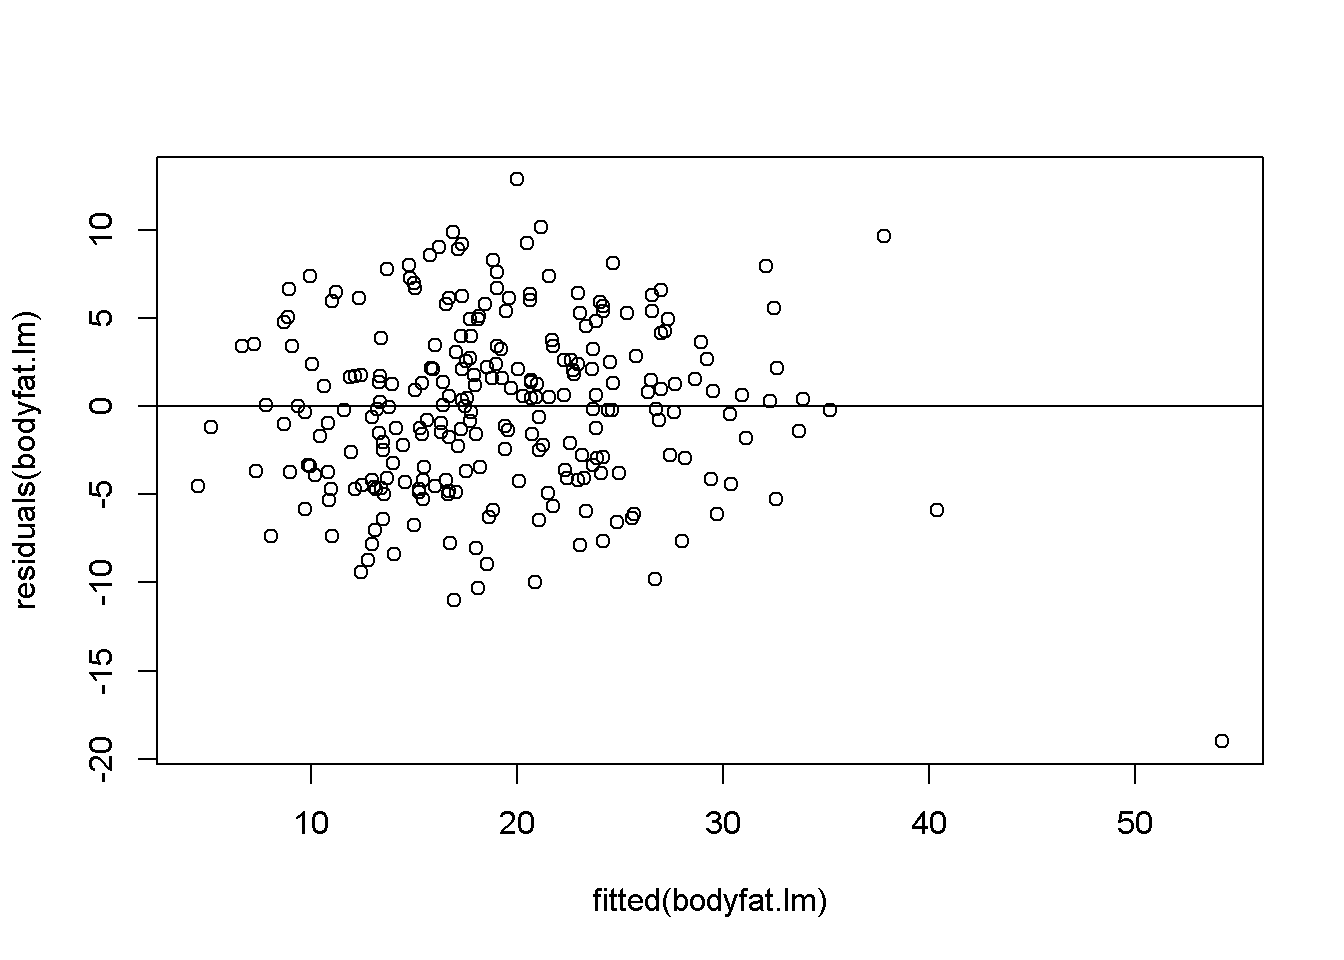
\includegraphics{04-regression-01-Bayesian-simple-regression_files/figure-latex/unnamed-chunk-3-1.pdf}

With the exception of the one observation for the individual with the
largest waist measurement, the residual plot suggests that the linear
regression is a reasonable approximation.

Furthermore, we can check the normal probability plot of the residuals
for the assumption of normally distributed errors:

\begin{Shaded}
\begin{Highlighting}[]
\KeywordTok{plot}\NormalTok{(bodyfat.lm, }\DataTypeTok{which =} \DecValTok{2}\NormalTok{)}
\end{Highlighting}
\end{Shaded}

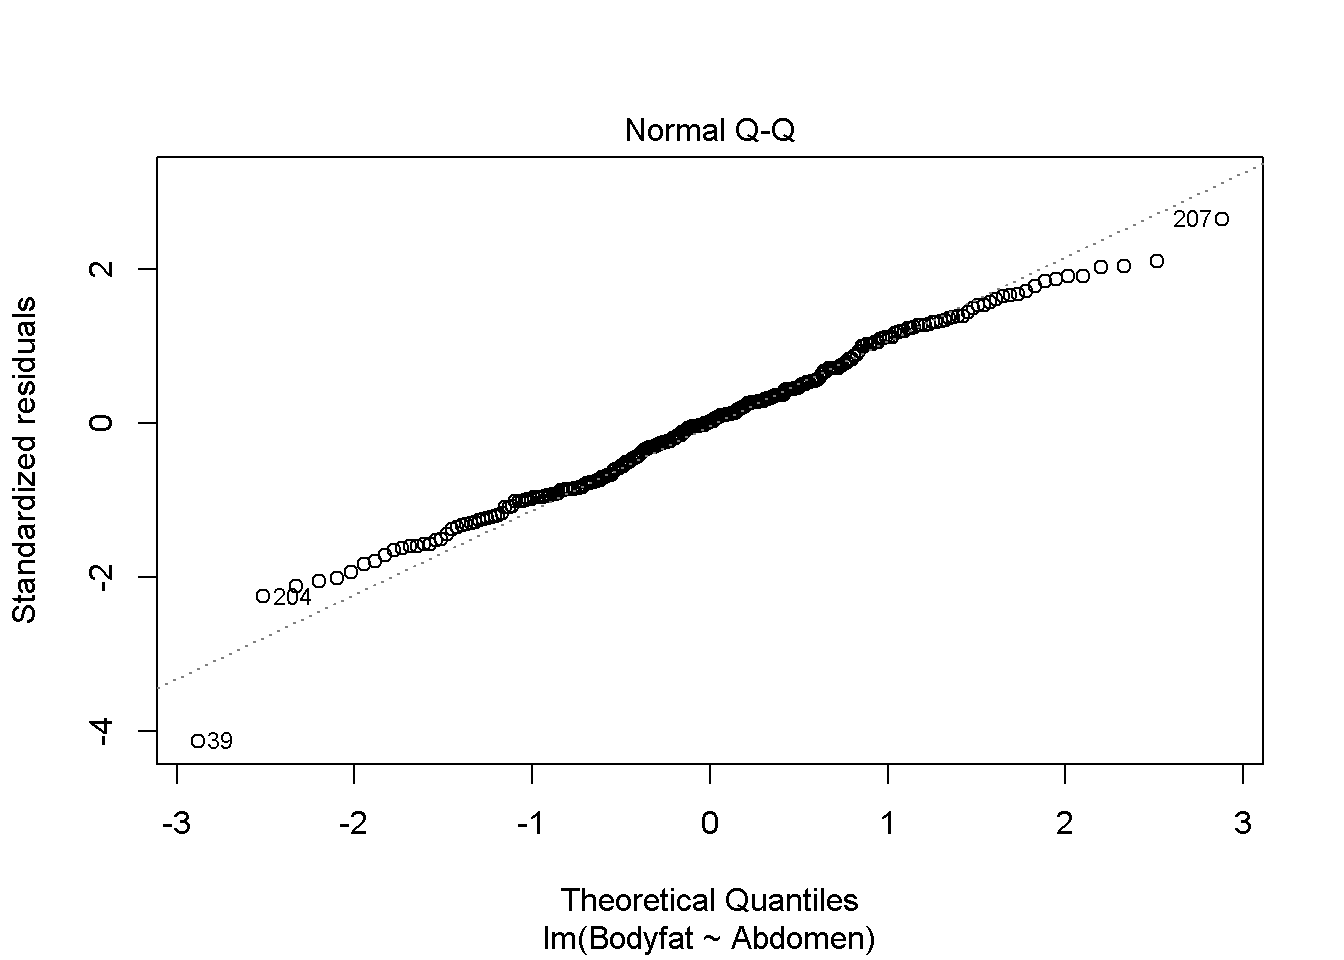
\includegraphics{04-regression-01-Bayesian-simple-regression_files/figure-latex/unnamed-chunk-4-1.pdf}

\subsection{Bayesian Simple Linear Regression Using Reference
Prior}\label{bayesian-simple-linear-regression-using-reference-prior}

Let us now turn to the Bayesian version and show how to obtain the
posterior distributions of \(\alpha\) and \(\beta\) under the reference
prior.

The Bayesian model starts with the same model as the classical
frequentist approach: \[ Y_i = \alpha + \beta X_i + \epsilon_i \] with
the assumption that the errors, \(\epsilon_i\), are independent and
identically distributed as normal random variables with mean zero and
constant variance \(\sigma^2\). This assumption is exactly the same as
the classical inference for testing and constructing confidence
intervals for \(\alpha\) and \(\beta\).

\section{Bayesian Multiple Linear
Regression}\label{bayesian-multiple-linear-regression}

\bibliography{packages,book,references}


\end{document}
